% Options for packages loaded elsewhere
\PassOptionsToPackage{unicode}{hyperref}
\PassOptionsToPackage{hyphens}{url}
%
\documentclass[
]{book}
\usepackage{lmodern}
\usepackage{amssymb,amsmath}
\usepackage{ifxetex,ifluatex}
\ifnum 0\ifxetex 1\fi\ifluatex 1\fi=0 % if pdftex
  \usepackage[T1]{fontenc}
  \usepackage[utf8]{inputenc}
  \usepackage{textcomp} % provide euro and other symbols
\else % if luatex or xetex
  \usepackage{unicode-math}
  \defaultfontfeatures{Scale=MatchLowercase}
  \defaultfontfeatures[\rmfamily]{Ligatures=TeX,Scale=1}
\fi
% Use upquote if available, for straight quotes in verbatim environments
\IfFileExists{upquote.sty}{\usepackage{upquote}}{}
\IfFileExists{microtype.sty}{% use microtype if available
  \usepackage[]{microtype}
  \UseMicrotypeSet[protrusion]{basicmath} % disable protrusion for tt fonts
}{}
\makeatletter
\@ifundefined{KOMAClassName}{% if non-KOMA class
  \IfFileExists{parskip.sty}{%
    \usepackage{parskip}
  }{% else
    \setlength{\parindent}{0pt}
    \setlength{\parskip}{6pt plus 2pt minus 1pt}}
}{% if KOMA class
  \KOMAoptions{parskip=half}}
\makeatother
\usepackage{xcolor}
\IfFileExists{xurl.sty}{\usepackage{xurl}}{} % add URL line breaks if available
\IfFileExists{bookmark.sty}{\usepackage{bookmark}}{\usepackage{hyperref}}
\hypersetup{
  pdftitle={Inferencia},
  pdfauthor={Rodrigo Zepeda-Tello y Luis Carlos Bernal},
  hidelinks,
  pdfcreator={LaTeX via pandoc}}
\urlstyle{same} % disable monospaced font for URLs
\usepackage{color}
\usepackage{fancyvrb}
\newcommand{\VerbBar}{|}
\newcommand{\VERB}{\Verb[commandchars=\\\{\}]}
\DefineVerbatimEnvironment{Highlighting}{Verbatim}{commandchars=\\\{\}}
% Add ',fontsize=\small' for more characters per line
\usepackage{framed}
\definecolor{shadecolor}{RGB}{248,248,248}
\newenvironment{Shaded}{\begin{snugshade}}{\end{snugshade}}
\newcommand{\AlertTok}[1]{\textcolor[rgb]{0.94,0.16,0.16}{#1}}
\newcommand{\AnnotationTok}[1]{\textcolor[rgb]{0.56,0.35,0.01}{\textbf{\textit{#1}}}}
\newcommand{\AttributeTok}[1]{\textcolor[rgb]{0.77,0.63,0.00}{#1}}
\newcommand{\BaseNTok}[1]{\textcolor[rgb]{0.00,0.00,0.81}{#1}}
\newcommand{\BuiltInTok}[1]{#1}
\newcommand{\CharTok}[1]{\textcolor[rgb]{0.31,0.60,0.02}{#1}}
\newcommand{\CommentTok}[1]{\textcolor[rgb]{0.56,0.35,0.01}{\textit{#1}}}
\newcommand{\CommentVarTok}[1]{\textcolor[rgb]{0.56,0.35,0.01}{\textbf{\textit{#1}}}}
\newcommand{\ConstantTok}[1]{\textcolor[rgb]{0.00,0.00,0.00}{#1}}
\newcommand{\ControlFlowTok}[1]{\textcolor[rgb]{0.13,0.29,0.53}{\textbf{#1}}}
\newcommand{\DataTypeTok}[1]{\textcolor[rgb]{0.13,0.29,0.53}{#1}}
\newcommand{\DecValTok}[1]{\textcolor[rgb]{0.00,0.00,0.81}{#1}}
\newcommand{\DocumentationTok}[1]{\textcolor[rgb]{0.56,0.35,0.01}{\textbf{\textit{#1}}}}
\newcommand{\ErrorTok}[1]{\textcolor[rgb]{0.64,0.00,0.00}{\textbf{#1}}}
\newcommand{\ExtensionTok}[1]{#1}
\newcommand{\FloatTok}[1]{\textcolor[rgb]{0.00,0.00,0.81}{#1}}
\newcommand{\FunctionTok}[1]{\textcolor[rgb]{0.00,0.00,0.00}{#1}}
\newcommand{\ImportTok}[1]{#1}
\newcommand{\InformationTok}[1]{\textcolor[rgb]{0.56,0.35,0.01}{\textbf{\textit{#1}}}}
\newcommand{\KeywordTok}[1]{\textcolor[rgb]{0.13,0.29,0.53}{\textbf{#1}}}
\newcommand{\NormalTok}[1]{#1}
\newcommand{\OperatorTok}[1]{\textcolor[rgb]{0.81,0.36,0.00}{\textbf{#1}}}
\newcommand{\OtherTok}[1]{\textcolor[rgb]{0.56,0.35,0.01}{#1}}
\newcommand{\PreprocessorTok}[1]{\textcolor[rgb]{0.56,0.35,0.01}{\textit{#1}}}
\newcommand{\RegionMarkerTok}[1]{#1}
\newcommand{\SpecialCharTok}[1]{\textcolor[rgb]{0.00,0.00,0.00}{#1}}
\newcommand{\SpecialStringTok}[1]{\textcolor[rgb]{0.31,0.60,0.02}{#1}}
\newcommand{\StringTok}[1]{\textcolor[rgb]{0.31,0.60,0.02}{#1}}
\newcommand{\VariableTok}[1]{\textcolor[rgb]{0.00,0.00,0.00}{#1}}
\newcommand{\VerbatimStringTok}[1]{\textcolor[rgb]{0.31,0.60,0.02}{#1}}
\newcommand{\WarningTok}[1]{\textcolor[rgb]{0.56,0.35,0.01}{\textbf{\textit{#1}}}}
\usepackage{longtable,booktabs}
% Correct order of tables after \paragraph or \subparagraph
\usepackage{etoolbox}
\makeatletter
\patchcmd\longtable{\par}{\if@noskipsec\mbox{}\fi\par}{}{}
\makeatother
% Allow footnotes in longtable head/foot
\IfFileExists{footnotehyper.sty}{\usepackage{footnotehyper}}{\usepackage{footnote}}
\makesavenoteenv{longtable}
\usepackage{graphicx,grffile}
\makeatletter
\def\maxwidth{\ifdim\Gin@nat@width>\linewidth\linewidth\else\Gin@nat@width\fi}
\def\maxheight{\ifdim\Gin@nat@height>\textheight\textheight\else\Gin@nat@height\fi}
\makeatother
% Scale images if necessary, so that they will not overflow the page
% margins by default, and it is still possible to overwrite the defaults
% using explicit options in \includegraphics[width, height, ...]{}
\setkeys{Gin}{width=\maxwidth,height=\maxheight,keepaspectratio}
% Set default figure placement to htbp
\makeatletter
\def\fps@figure{htbp}
\makeatother
\setlength{\emergencystretch}{3em} % prevent overfull lines
\providecommand{\tightlist}{%
  \setlength{\itemsep}{0pt}\setlength{\parskip}{0pt}}
\setcounter{secnumdepth}{5}
\usepackage{booktabs}
\usepackage[framemethod=TikZ]{mdframed}
\usepackage{xcolor}
\definecolor{ejemplocolor}{HTML}{0A7000}
\definecolor{recuadrocolor}{HTML}{3DB295}
\definecolor{teoremacolor}{HTML}{900C3F}
\definecolor{propiedadescolor}{HTML}{C301AC}
\definecolor{importantecolor}{HTML}{FF0000}
\definecolor{corolariocolor}{HTML}{0CABAD}
\definecolor{lemacolor}{HTML}{0BA50B}
\definecolor{ejerciciocolor}{HTML}{183283}
\definecolor{definicioncolor}{HTML}{183283}
\definecolor{formulacolor}{HTML}{137AA4}


\newenvironment{Ejemplo}
{\begin{mdframed}[
  linecolor=ejemplocolor,
  skipabove=12pt,
  skipbelow=12pt,
  roundcorner=20pt,
  splittopskip=2\topsep]}
{\end{mdframed}}

\newenvironment{Definicion}
{\begin{mdframed}[
  linecolor=definicioncolor,
  skipabove=12pt,
  skipbelow=12pt,
  roundcorner=20pt,
  splittopskip=2\topsep]}
{\end{mdframed}}

\newenvironment{Recuadro}
{\begin{mdframed}[
  linecolor=recuadrocolor,
  skipabove=12pt,
  skipbelow=12pt,
  roundcorner=20pt,
  splittopskip=2\topsep]}
{\end{mdframed}}

\newenvironment{Teorema}
{\begin{mdframed}[
  linecolor=teoremacolor,
  skipabove=12pt,
  skipbelow=12pt,
  roundcorner=20pt,
  splittopskip=2\topsep]}
{\end{mdframed}}

\newenvironment{Propiedades}
{\begin{mdframed}[
  linecolor=propiedadescolor,
  skipabove=12pt,
  skipbelow=12pt,
  roundcorner=20pt,
  splittopskip=2\topsep]}
{\end{mdframed}}

\newenvironment{Importante}
{\begin{mdframed}[
  linecolor=importantecolor,
  skipabove=12pt,
  skipbelow=12pt,
  roundcorner=20pt,
  splittopskip=2\topsep]}
{\end{mdframed}}

\newenvironment{Corolario}
{\begin{mdframed}[
  linecolor=corolariocolor,
  skipabove=12pt,
  skipbelow=12pt,
  roundcorner=20pt,
  splittopskip=2\topsep]}
{\end{mdframed}}

\newenvironment{Lema}
{\begin{mdframed}[
  linecolor=lemacolor,
  skipabove=12pt,
  skipbelow=12pt,
  roundcorner=20pt,
  splittopskip=2\topsep]}
{\end{mdframed}}

\newenvironment{Ejercicio}
{\begin{mdframed}[
  linecolor=ejerciciocolor,
  skipabove=12pt,
  skipbelow=12pt,
  roundcorner=20pt,
  splittopskip=2\topsep]}
{\end{mdframed}}

\newenvironment{Formula}
{\begin{mdframed}[
  linecolor=formulacolor,
  skipabove=12pt,
  skipbelow=12pt,
  roundcorner=20pt,
  splittopskip=2\topsep]}
{\end{mdframed}}
\usepackage{booktabs}
\usepackage{longtable}
\usepackage{array}
\usepackage{multirow}
\usepackage{wrapfig}
\usepackage{float}
\usepackage{colortbl}
\usepackage{pdflscape}
\usepackage{tabu}
\usepackage{threeparttable}
\usepackage{threeparttablex}
\usepackage[normalem]{ulem}
\usepackage{makecell}
\usepackage{xcolor}
\usepackage[]{natbib}
\bibliographystyle{apalike}

\title{Inferencia}
\author{Rodrigo Zepeda-Tello y Luis Carlos Bernal}
\date{2021-01-14}

\begin{document}
\maketitle

{
\setcounter{tocdepth}{1}
\tableofcontents
}
\hypertarget{intro}{%
\chapter{Introducción}\label{intro}}

\hypertarget{estaduxedstica-y-muestras}{%
\section{Estadística y muestras}\label{estaduxedstica-y-muestras}}

La \href{https://plato.stanford.edu/entries/statistics/\#StaInd}{enciclopedia Stanford de filosofía} establece la siguiente definición de estadística\footnote{Traducción y subrayado de Rodrigo}.

\begin{Definicion}
\textbf{Estadística} La estadística es una disciplina matemática y
conceptual que se enfoca en la relación entre datos e hipótesis. Los
datos son registros de observaciones o eventos en un estudio científico,
por ejemplo, un conjunto de mediciones de individuos de una población.
Los datos que son obtenidos se conoce como la muestra, datos muestrales,
o simplemente los datos, y todas las posibles muestras posibles en un
estudio forman una colección llamada el espacio muestra. Las hipótesis,
por su parte, son enunciados generales sobre el sistema objetivo de la
investigación científica, por ejemplo, expresar un hecho general sobre
todos los individuos en la población. Una hipótesis estadística es un
enunciado general que puede ser expresada como una distribución de
probabilidad sobre el espacio muestral, es decir, ésta determina una
probabilidad para cada una de las posibles muestras.
\end{Definicion}

De manera breve, la estadística es una disciplina que se encarga de, a través de muestras (cuantificadas como datos), describir el mundo. Y hay muchas cosas por describir: asociaciones, causalidad, realizar predicciones, establecer mecanismos de funcionamiento de objetos, etc. Es así como se establece su objetivo el cual de acuerdo con \citet{wackerly} es:

\begin{quote}
realizar una inferencia sobre la población con base en la información contenida en una muestra de dicha población y proveer una medida asociada de qué tan buena es la inferencia.
\end{quote}

Dentro de la definición previa y objetivos hay que destacar varios términos que son de importancia. La primera es la \textbf{población}, cualquier conjunto (no vacío) de objetos. Una \textbf{población} es lo más general posible, no necesariamente involucra personas o seres vivos. Algunos ejemplos de poblaciones incluyen: las personas que viven en Guatemala (si me interesa saber algo de los guatemaltecos en general), los árboles del Amazonas (si quiero saber cosas de ecología), los perros callejeros en Ciudad de México, los consumidores de una marca de cereal, los coches que transitan por Dubai, los granos de arena en una playa específica de Cancún, las células T dentro de los seres humanos o los metales pesados.

Más relevante que la población (para nuestros propósitos) es la \textbf{población objetivo} El conjunto de elementos que formarán parte del estudio. Definir la \textbf{población objetivo} es complicado en algunas situaciones; por ejemplo, si se desea saber si \emph{los mexicanos} están a favor o en contra de legalizar la marihuana hay que establecer quiénes son \emph{los mexicanos}. ¿Cuentan las personas con nacionalidad mexicana que residen en el extranjero? ¿Cuentan los menores de edad? ¿Qué pasa con los extranjeros que son residentes? De nuevo, la población objetivo no necesariamente son personas, es sólo aquello que nos interesa medir.

Idealmente el estudio estadístico sería sobre la población objetivo. Por ejemplo, si nos interesa estudiar la evolución de los enfermos de VIH, la \textbf{población objetivo} serían los enfermos. Sin embargo, en el mundo real es imposible conseguir a toda la población objetivo (dentro de los enfermos, por ejemplo, están aquellos que aún no saben que tienen la enfermedad y no acudirían a nuestro estudio). La \textbf{población muestreada} resulta de esta dificultad. La \textbf{población muestreada} es el conjunto de elementos sobre los cuales se construyó la muestra para el análisis estadístico. En el caso de los enfermos de VIH la \textbf{población muestreada} podrían ser las personas que para una fecha específica habían sido diagnosticadas (y nos olvidamos de quienes desconocen su diagnóstico) o toda la población mexicana (y llevamos kits de diagnóstico con nosotros cuando diagnostiquemos). En encuestas de consumo, por ejemplo, usualmente no se muestrean zonas remotas o de muy bajos recursos por lo que la \textbf{población muestreada} no coincide con la \textbf{población objetivo} (todos los consumidores) sino que son sólo los consumidores de mayor poder adquisitivo. En encuestas de elecciones si bien la población objetivo son \emph{todas las personas que voten el día de la elección}, como la mayoría se hacen \emph{antes} de la elección (exceptuando las de salida) entonces se aproxima la definición de \emph{votante} buscando incluir sólo aquellos que estén registrados en el padrón electoral o bien aquellos que al ser encuestados digan que \emph{sí} van a votar. Aquí la \textbf{población muestreada} tampoco coincide con la objetivo.

Una \textbf{muestra} es un subconjunto de la población muestreada. Si la muestra coincide con la población muestreada (es decir, muestreaste a todo el mundo) se dice que es un \textbf{censo}. Si se tiene un censo se conoce TODA la población por lo que no es necesario hacer ningún análisis de inferencia (ya sabes todo de todos). Puedes realizar predicciones o descripciones. Ejemplos de censos son las encuestas de fin de cursos, las calificaciones de todo un grupo o el registro de todas las compras de todas las personas en una tienda en línea.

\begin{quote}
\textbf{Ojo} No hay que confundir la definición de \textbf{muestra} con la definición estadística de \textbf{muestra aleatoria} (ver más adelante) la cual es un tipo muy específico de muestra obtenida bajo reglas restrictivas.
\end{quote}

Finalmente hay que definir \textbf{inferencia}, el propósito de estas notas. Para ello usaremos el ejemplo y una versión adaptada de la definición de \citet{boghossian2014inference}. Considera que sabes dos verdades:

\begin{enumerate}
\def\labelenumi{\arabic{enumi}.}
\item
  Llovió anoche
\item
  Cuando llueve el suelo se moja
\end{enumerate}

por lo que esta mañana \emph{infieres} que el suelo estará mojado y sales de tu casa con botas y no con chanclas. El proceso de \emph{inferir} parece una consecuencia lógica de las premisas 1 y 2 pero no lo es exactamente: hoy es otro día y si hizo suficiente calor en la noche el agua pudo haberse evaporado del suelo. De ahí que definamos inferencia como:

\begin{quote}
Realizar un juicio el cual se explica a partir de premisas que suponemos verdaderas.
\end{quote}

En particular \textbf{la inferencia estadística} será la rama de la estadística cuyo propósito es

\begin{quote}
Realizar juicios probabilísticos a partir de datos que suponemos verdaderos.
\end{quote}

Aquí es necesario desglosar un poco la definición:

\begin{itemize}
\item
  Se habla de \textbf{juicios probabilísticos} pues nuestros juicios nunca van a ser tan certeros como \texttt{el\ suelo\ està\ mojado}. Más bien van a ser del estilo \texttt{hay\ una\ probabilidad\ muy\ alta\ de\ que\ el\ suelo\ esté\ mojado} o \texttt{nueve\ de\ cada\ diez\ veces\ el\ suelo\ estará\ mojado}.
\item
  La \textbf{suposición de verdad} de los datos es muy relevante. Imagina el siguiente experimento: tu amiga borracha durante una fiesta se le ocurre que, de la nada, desarrolló poderes de psíquica y puede adivinar el futuro resultado de una moneda (cara o cruz). Tiras una moneda diez veces y todas las veces tu amiga hace una predicción correcta. \emph{Considerando los datos como verdad concluirías que tu amiga es psíquica}. Una observación a profundidad de la moneda quizá te revele que es una moneda truqueada que siempre cae en cara. En ese momento cambiarías la \textbf{suposición de verdad} de los datos y la inferencia de que tu amiga es psíquica.
\end{itemize}

A lo largo de este libro aprenderemos lo básico para realizar inferencias estadísticas: observar datos y suponer verdades a partir de ellos. Tristemente la estadística nunca nos va a poder dar la verdad absoluta pero, si lo hacemos bien, es quizá lo más cerca que podamos estar de ella.

\hypertarget{modelos}{%
\section{Modelos}\label{modelos}}

La estadística funciona a partir de la construcción de \textbf{modelos}. Estos pretenden ser una forma de describir el mundo mediante teoría de la probabilidad y lo que se busca es utilizar dicha teoría para realizar inferencias. Estos modelos teóricos representan la forma en la que suponemos funciona la población. Para propósitos de estas notas diremos que los modelos viven \emph{en el mundo de los modelos} o \emph{mundo de las ideas}. Los datos observados, para poder distinguirlos, viven en \emph{el mundo real}. Muchos de los modelos (no todos) se componen de \textbf{parámetros} que requieren para poder funcionar los cuales son estimados mediante \textbf{estadísticos} que se construyen a partir de los datos.

Para nuestros propósitos, los modelos que usaremos siempre construirán una población de la siguiente forma:

\begin{Definicion}
\hypertarget{poblaciuxf3n}{%
\subsubsection{Población}\label{poblaciuxf3n}}

Una población es un conjunto no vacío de variables (o vectores)
aleatorias. \[
\mathcal{X} = \{ X_1, X_2, \dots \}
\]
\end{Definicion}

Una población no necesariamente es finita. Por ejemplo, si nos interesa saber el tiempo que tarda un cliente en ser atendido en una llamada telefónica al banco quizá podemos suponer que la llamada telefónica tiene una duración descrita por un modelo \(\text{Exponencial}(\lambda)\). La población sería el conjunto infinito de todas las posibles llamadas telefónicas que se pueden realizar bajo este modelo. Por otro lado, un ejemplo finito de una población, son las caras de una moneda en un experimento donde busquemos, para una moneda específica, si caen más caras que cruces (cae más de un lado que del otro).

Una \textbf{muestra} es cualquier subconjunto (posiblemente infinito también) de la población.

\begin{Definicion}
\hypertarget{muestra}{%
\subsubsection{Muestra}\label{muestra}}

Una muestra \(\mathcal{M}\) de una población \(\mathcal{X}\) es
cualquier subconjunto no vacío de \(\mathcal{X}\). Es decir,
\(\mathcal{M}\) es una muestra de \(\mathcal{X}\) si: \[
 \mathcal{M} \subseteq \mathcal{X}
\]
\end{Definicion}

Pocas veces hablaremos de \emph{muestras} de manera general y nos enfocaremos, sobre todo, en \textbf{muestras aleatorias}:

\begin{Definicion}
\hypertarget{muestra-aleatoria}{%
\subsubsection{Muestra aleatoria}\label{muestra-aleatoria}}

Una muestra aleatoria de tamaño \(n\), \(\mathcal{X}_{(n)}\), de una
población \(\mathcal{X}\) es un subconjunto finito (de tamaño \(n\)), no
vacío de \(\mathcal{X}\) donde sus elementos son \textbf{variables
aleatorias independientes idénticamente distribuidas}. Es decir,
\(\mathcal{X}_{(n)}\) es una muestra de \(\mathcal{X}\) si:

\begin{enumerate}
\def\labelenumi{\arabic{enumi}.}
\item
  \textbf{Es una muestra}: \(\mathcal{X}_{(n)} \subseteq \mathcal{X}\),
\item
  \textbf{de tamaño \(n\)}:
  \(\textrm{Cardinalidad}\Big( \mathcal{X}_{(n)} \Big) = n\),
\item
  \textbf{con variables independientes}: si
  \(X_i, X_j \in \mathcal{X}_{(n)}\) entonces
  \(\mathbb{P}(X_i \in A , X_j \in B) = \mathbb{P}(X_i \in A)\cdot\mathbb{P}(X_j \in B)\)
  para \(A,B\) conjuntos \emph{medibles},
\item
  \textbf{idénticamente distribuidas}: para todo \(i = 1,2,\dots, n\) se
  tiene que \(X_i\) tiene función de distribución acumulada \(F_X\).
\end{enumerate}
\end{Definicion}

El punto 4. de la definición pide que todas las variables descritas tengan la misma distribución. Por ejemplo, podemos pedir que todas sean exponenciales con el mismo parámetro o todas sean gamma con los mismos parámetros. El punto es que todas las variables aleatorias estén descritas con el mismo modelo y sean independientes entre sí.

El punto 3. de la definición puede escribirse de otras formas más amigables, por ejemplo, si suponemos que las variables aleatorias son continuas y tienen densidad \(f_X\) entonces la independencia puede escribirse como:
\[
f_X(x_i, x_j) = f_X(x_i) \cdot f_X(x_j)
\]
mientras que si son discretas con función de masa de probabilidad \(p_X\) tenemos:
\[
p_X(x_i, x_j) = p_X(x_i) \cdot p_X(x_j)
\]

La \textbf{muestra observada} así como \textbf{la muestra aleatoria observada} es el conjunto de \emph{datos} que realmente viste. Mientras que la \textbf{muestra} y la \textbf{muestra aleatoria} viven \emph{en el mundo de los modelos} y son variables aleatorias (constructos teóricos, como sabes, bastante complejos), la \textbf{muestra observada} es lo que se midió. Antes de dar la definición veamos un ejemplo con un dado.

\begin{Ejemplo}
\hypertarget{tiro-de-un-dado}{%
\subsubsection{Tiro de un dado}\label{tiro-de-un-dado}}

Se realiza un experimento para saber si un dado es justo (todos los
lados tienen la misma probabilidad). Para ello se tira el dado
\(n = 10\) veces y se registran los tiros: \(2,6,1,3,3,3,5,1,3,2\).

\emph{Mundo del modelo}

La población en este caso es el conjunto infinito de todos los posibles
tiros del dado. De ese conjunto obtenemos una muestra aleatoria de
tamaño \(n = 10\) (suponemos que los tiros son independientes entre sí)
dada por: \[
X_{(n)} = \{ X_1, X_2, X_3, \dots, X_{10}\}
\] donde \(X_i\) tiene la siguiente distribución: \[
\mathbb{P}(X_i = z) = 
\begin{cases}
p_1  \text{ si } z = 1 \\
p_2  \text{ si } z = 2 \\
p_3  \text{ si } z = 3 \\
p_4  \text{ si } z = 4 \\
p_5  \text{ si } z = 5 \\
p_6  \text{ si } z = 6 \\
0  \text{ en otro caso.}
\end{cases}
\] donde \(\sum_{k = 1}^n p_k = 1\) y \(p_{k} \geq 0\) para todo \(k\).
Lo que interesa en este estudio es \emph{inferir} quiénes son las
\(p_k\) para determinar si es más probable que caiga en un lado que en
otro. Las \(p_k\) se conocen como parámetros.

\emph{Mundo real}

Ya en la realidad en esos \(10\) tiros no observamos cualquier cosa,
observamos valores específicos que hacen que \textbf{la muestra
aleatoria observada} sea: \[
s_n = \{x_1, x_2, \dots, x_{10} \} = \{2,6,1,3,3,3,5,1,3,2\}.
\] Por supuesto que repitiendo el experimento (volviendo a tirar el dado
10 veces) lo más probable es que la \textbf{muestra aleatoria observada}
cambie (y veamos otros números) pero el modelo, reflejado en la
\textbf{muestra aleatoria} (teórica), permanezca inmutable. Una forma de
estimar las probabilidades podría ser mediante proporciones y calcular,
por ejemplo, la probabilidad de que aparezca \(1\) como: \[
\hat{p}_1 = \frac{\text{Veces que aparece 1}}{n} = \frac{2}{10}
\] En este caso, \(\hat{p}_1\) dado por \(\frac{2}{10}\) es un
\textbf{estimador observado} de la verdadera probabilidad \(p_1\) que
vive en el mundo de los modelos (y jamás podremos conocer)
\end{Ejemplo}

Armados con el ejemplo anterior realicemos la definición de las muestras observadas:

\begin{Definicion}
\hypertarget{muestra-observada}{%
\subsubsection{Muestra observada}\label{muestra-observada}}

Una muestra observada es una colección no vacía de valores codificados
como números reales los cuales corresponden a realizaciones de una
muestra \(\mathcal{X}\). Usualmente la denotamos: \[
s = \{ x_1, x_2, \dots\}
\] donde las \(x_i\) \textbf{NO SON VARIABLES ALEATORIAS} sino que son
datos \textbf{fijos} ya observados.
\end{Definicion}

\begin{Definicion}
\hypertarget{muestra-aleatoria-observada}{%
\subsubsection{Muestra aleatoria
observada}\label{muestra-aleatoria-observada}}

Una muestra aleatoria observada es una colección no vacía de tamaño
\(n\) de valores codificados como números reales los cuales corresponden
a realizaciones de una muestra aleatoria \(\mathcal{X}_{(n)}\). En
particular suponemos que \(x_1\) es el valor observado de la variable
aleatoria \(X_1\), \(x_2\) es el valor observado de la variable
aleatoria \(X_2\) y así sucesivamente. Generalmente la denotamos por: \[
s_{(n)} = \{ x_1, x_2, \dots, x_n\}
\] donde las \(x_i\) \textbf{NO SON VARIABLES ALEATORIAS} sino que son
datos \textbf{fijos} ya observados.
\end{Definicion}

Veamos un segundo ejemplo:

\begin{Ejemplo}
\hypertarget{cantidad-de-personas-que-llegan-a-una-tienda}{%
\subsubsection{Cantidad de personas que llegan a una
tienda}\label{cantidad-de-personas-que-llegan-a-una-tienda}}

En muchos casos la llegada de personas se supone que sigue una
distribución Poisson. En este caso nos interesa estimar el número
promedio de personas por día que hay en una tienda de la cual se han
medido las siguientes cantidades (por día). Suponemos que las llegadas
son independientes entre sí (la cantidad de gente que llegó un día no
influye en la cantidad que llegó el otro).

\begin{longtable}[]{@{}ll@{}}
\toprule
\textbf{Día} & \textbf{Número de personas}\tabularnewline
\midrule
\endhead
1 & 50\tabularnewline
2 & 45\tabularnewline
3 & 60\tabularnewline
4 & 65\tabularnewline
5 & 55\tabularnewline
6 & 40\tabularnewline
\bottomrule
\end{longtable}

\emph{Mundo del modelo}

La población en este caso es el conjunto infinito de todas las posibles
formas en que en un día pueden llegar personas. De ese conjunto
obtenemos una muestra aleatoria de tamaño \(n = 6\) (suponemos que las
observaciones son independientes entre sí) dada por: \[
X_{(n)} = \{ X_1, X_2, X_3, X_4, X_5, X_6\}
\] donde las \(X_i \sim \text{Poisson}(\lambda)\) (todas con el mismo
\(\lambda\)). Recordamos que la media de una Poisson es \(\lambda\) por
lo que el \textbf{parámetro} que nos interesa estimar es \(\lambda\).

\emph{Mundo real}

A partir de las \(6\) llegadas observadas construimos \textbf{la muestra
aleatoria observada}: \[
s_n = \{x_1, x_2, x_3, x_4, x_5, x_6 \} = \{50, 45, 60, 65, 55, 40\}.
\] Una forma de estimar la media \(\lambda\) es mediante el siguiente
\textbf{estimador observado}: \[
\hat{\lambda} = \frac{1}{6} \sum_{i = 1}^6 x_i = 52.5
\] Ojo, esto no significa que \(\lambda\) \emph{sea} \(52.5\). Significa
que nuestra hipótesis de quién es \(\lambda\) es \(52.5\) y que
esperaríamos la próxima vez en la tienda \(52\) ó \(53\) personas. En el
mundo real \emph{quién sabe cuánto vale \(\lambda\)} , nuestra hipótesis
es que vale \(52.5\) pero eso no necesarimente es la realidad.
\end{Ejemplo}

Como ya establecimos, muchas veces el modelo utiliza un \textbf{parámetro} el cual es desconocido. A partir de los datos construimos un \textbf{estimador observado} el cual es nuestra hipótesis del verdadero valor del parámetro. En general va a ser imposible que le atinemos al \emph{verdadero} valor del parámetro pero la idea es que el \textbf{estimador observado} esté lo suficientemente cerca. En el ejemplo anterior nos gustaría, por ejemplo, que el verdadero parámetro quizá fuera \(\lambda = 52\) ó \(\lambda = 54\) pero nos sacaría mucho de onda que el parámetro real fuera \(\lambda = 1000000\).

\begin{Definicion}
\hypertarget{distirbuciuxf3n-paramuxe9trica}{%
\subsubsection{Distirbución
paramétrica}\label{distirbuciuxf3n-paramuxe9trica}}

Una función de distirbución acumulada es una \textbf{distribución
paramétrica} con parámetro \(\vec{\theta}\) si dada una colección de
distribuciones \[
\{ F_{\vec{\theta}} | \theta \in \Theta \}
\] determinar \(\vec{\theta}\) determina la distribución. Es decir, la
familia de distribuciones está indizada por \(\vec{\theta}\). A
\(\vec{\theta}\) se le conoce como el \textbf{parámetro} o
\textbf{vector de parámetros}.
\end{Definicion}

La definición anterior suena muy compleja sin embargo los ejemplos ya los conocemos.

\begin{Ejemplo}
\hypertarget{la-normal}{%
\subsubsection{La normal}\label{la-normal}}

La distribución normal es una distribución paramétrica con \[
\vec{\theta} = (\mu, \sigma^2)^T
\] el vector de parámetros dado por la media y la varianza.
\end{Ejemplo}

\begin{Ejemplo}
\hypertarget{la-exponencial}{%
\subsubsection{La exponencial}\label{la-exponencial}}

La distribución exponencial es una distribución paramétrica con \[
\theta = \lambda
\] el parámetro que establece la tasa de la exponencial.
\end{Ejemplo}

\begin{Ejemplo}
\hypertarget{la-normal-con-varianza-1}{%
\subsubsection{La normal con varianza
1}\label{la-normal-con-varianza-1}}

La distribución normal con varianza 1 es una distribución paramétrica
con \[
\theta = \mu
\] En este caso la varianza es conocida (\(\sigma^2 = 1\)) pero la media
no por eso sólo la media es el parámetro.
\end{Ejemplo}

Podemos entonces definir un \textbf{estimador}:

\begin{Definicion}
\hypertarget{estimador}{%
\subsubsection{Estimador}\label{estimador}}

Dada una distribución paramétrica \(F_{\theta}\) con parámetro
\(\theta\) un estimador \(\hat{\theta}\) de \(\theta\) es una variable
aleatoria que se construye como función de la muestra aleatoria: \[
\hat{\theta}: \mathcal{X}_{(n)} \to \Theta
\] Como \(\hat{\theta}\) es una función de la muestra aleatoria entonces
puede representarse como: \[
\hat{\theta} = \hat{\theta}(X_1, X_2, \dots, X_n)
\]
\end{Definicion}

Dado un conjunto de datos, el \textbf{estimador observado de \(\theta\)} es el estimador \(\hat{\theta}\) de \(\theta\) evaluado en los datos.

\begin{Definicion}
\hypertarget{estimador-observado}{%
\subsubsection{Estimador observado}\label{estimador-observado}}

Dada una distribución paramétrica \(F_{\theta}\) con parámetro
\(\theta\) con estimador \(\hat{\theta}\) y datos observados
\(s_{(n)} = \{x_1, x_2, \dots, x_n\}\) el \textbf{estimador observado}
corresponde a la evaluación de \(\hat{\theta}\) en \(s_{(n)}\); es
decir: \[
\hat{\theta}(x_1, x_2, \dots, x_n)
\]
\end{Definicion}

Veamos ejemplos para entender mejor cómo funciona esto.

\begin{Ejemplo}
\hypertarget{tiros-de-una-moneda}{%
\subsubsection{Tiros de una moneda}\label{tiros-de-una-moneda}}

Se tiene una moneda que cae más de un lado que del otro. Interesa
estimar \(p\) la probabilidad de que caiga cruz. Para ello se toma una
\textbf{muestra aleatoria} de \(5\) tiros de la moneda: \[
X_{(n)} = \{X_1, X_2, \dots, X_{5} \}
\] Suponemos que los tiros son independientes. El modelo entonces
implicaría que \[
X_i \sim \text{Bernoulli}(p)
\] para cada \(i = 1, 2, \dots, 5\). Si codificamos cruz como \(1\) y
cara como \(0\), la \textbf{muestra aleatoria observada} es: \[
s_{(n)} = \{1,1,1,0,1\} = \{x_1, x_2, \dots, x_5\}
\] donde tuvimos tres cruces continuas, luego una cara y finalmente una
cruz. Una opción de estimador observado sería contar la proporción de
cruces haciendo: \[
\hat{\theta}(x_1, \dots, x_5) = \frac{1}{n} \sum_{k = 1}^n x_i = \frac{4}{5}
\] de donde diríamos que nuestra hipótesis de cuánto vale el parámetro
\(p\) es \(4/5\). Por otro lado, el \textbf{estimador} teórico es: \[
\hat{\theta}(X_1, \dots, X_5) = \frac{1}{n} \sum_{k = 1}^n X_i 
\] el cual tiene una distribución de probabilidad sencilla pues
\(\sum_{k = 1}^n X_i \sim \textrm{Binomial}(n,p)\). Particularmente
podemos calcular su valor esperado, por ejemplo, \[
\mathbb{E}\Big[  \hat{\theta}(X_1, \dots, X_5) \Big]  =  \mathbb{E}\Big[  \frac{1}{n} \sum_{k = 1}^n X_i  \Big] = \frac{1}{n}\sum_{k = 1}^n \mathbb{E}\Big[X_i \Big] = \frac{1}{n}\sum_{k = 1}^n  p = \frac{1}{n} np = p
\] lo cual implica que el estimador, en promedio, devolvería el
parámetro que nos interesa (esta propiedad se conoce como \emph{ser
insesgado} y lo veremos más adelante).
\end{Ejemplo}

\begin{Ejemplo}
\hypertarget{error-de-mediciuxf3n-de-una-app}{%
\subsubsection{Error de medición de una
app}\label{error-de-mediciuxf3n-de-una-app}}

Una app que se dedica a medir la altura de edificios mediante la toma de
videos tiene un error de medición con distribución normal y cuya
varianza es \(1\). Interesa determinar el error de medición promedio, el
parámetro \(\mu\). Para ello se toman videos y se miden edificios para
obtener una colección de 7 errores de medición independientes en la
siguiente \textbf{muestra aleatoria}: \[
X_{(n)} = \{X_1, X_2, \dots, X_{5} \}
\] El modelo es \[
X_i \sim \text{Normal}(\mu, 1)
\] para cada \(i = 1, 2, \dots, 7\). Si los datos fueron:

\begin{longtable}[]{@{}ll@{}}
\toprule
\textbf{Edificio} & \textbf{Error de medición}\tabularnewline
\midrule
\endhead
Bellas Artes & 12.11\tabularnewline
Torre Latinoamericana & 40.54\tabularnewline
Catedral Metropolitana & 22.07\tabularnewline
Palacio Nacional & 15.22\tabularnewline
Rectoría de la UNAM & 45.18\tabularnewline
Guerrero Chimalli & 33.39\tabularnewline
Estadio Azteca & 41.76\tabularnewline
\bottomrule
\end{longtable}

la \textbf{muestra aleatoria observada} en este caso correspondió : \[
s_{(n)} = \{12.11,40.54,22.07,15.22,45.18, 33.39, 41.76\} = \{x_1, x_2, \dots, x_7\}
\] Una opción de estimador observado sería calcular la media muestral
haciendo: \[
\hat{\theta}(x_1, \dots, x_7) = \frac{1}{n} \sum_{k = 1}^n x_i = 30.03857
\] de donde diríamos que nuestra hipótesis de cuánto vale el parámetro
\(\mu\) es \(30.03857\). Por otro lado, el \textbf{estimador} teórico
es: \[
\hat{\theta}(X_1, \dots, X_7) = \frac{1}{n} \sum_{k = 1}^n X_i 
\] tiene una distribución de probabilidad sencilla pues sabemos que
\(\sum_{k = 1}^n X_i \sim \textrm{Normal}(\mu,\sigma^2)\).
Particularmente podemos calcular su valor esperado, por ejemplo, \[
\mathbb{E}\Big[  \hat{\theta}(X_1, \dots, X_7) \Big]  =  \mathbb{E}\Big[  \frac{1}{n} \sum_{k = 1}^n X_i  \Big] = \frac{1}{n}\sum_{k = 1}^n \mathbb{E}\Big[X_i \Big] = \frac{1}{n}\sum_{k = 1}^n  \mu = \frac{1}{n} n\mu = \mu
\] lo cual implica que el estimador, en promedio, devolvería el
parámetro que nos interesa (este también es \emph{insesgado}).
\end{Ejemplo}

A modo de resumen y para concluir este capítulo introductorio, veamos un ejemplo más desarrollado de inferencia estadística.

\hypertarget{inferencia-estaduxedstica-ejemplo.}{%
\section{Inferencia estadística: ejemplo.}\label{inferencia-estaduxedstica-ejemplo.}}

Se tiene una caja con cinco pelotas de colores rojo \(R\) y azul \(A\). Las pelotas son indistinguibles\footnote{Pelotas distinguibles, por ejemplo, tendrían números distintos o serían de materiales diferentes o con marcas específicas para saber que una azul es distinta de la otra.} entre sí salvo por el color. Se desconoce exactamente la proporción de colores de la caja (es decir no se sabe cuál de las siguientes opciones es: \(\{ R, R, R, R, R\}\), \(\{ R, R, R, R, A\}\), \(\{ R, R, R, A, A\}\), \(\{ R, R, A, A, A\}\), \(\{ R, A, A, A, A\}\), \(\{ A, A, A, A, A\}\)) y eso es lo que se desea determinar. Para ello se extrae una bola, se anota que su color fue rojo, \(R\), y se devuelve a la caja. Se extrae otra bola (que, pudo haber sido la misma que la inicial, recuerda que las bolas son indistinguibles y que la anterior se devolvió a la caja), se anota que su color fue rojo \(R\) y se devuelve a la caja. Finalmente en la tercera extracción sale una pelota azul \(A\). Los datos observados (y ordenados) son los siguientes \(( R, R, A)\). Hay dos estimadores posibles de la probabilidad de que salga rojo \(p\) que podemos calcular a partir de la \textbf{muestra aleatoria} ordenada \(( R, R, A)\)

\hypertarget{estimador-de-momentos}{%
\subsection{Estimador de momentos}\label{estimador-de-momentos}}

Una opción es estimar la probabilidad de que salga rojo, \(p\), mediante el conteo de cuántos rojos salieron divididos entre el total de extracciones. En este caso tendríamos el estimador evaluado en la muestra:
\[
\hat{p}_M = \frac{2}{3}
\]
Aquí una nota bien importante: es imposible \emph{(¿por qué?)} que en la vida real la probabilidad \(p\) de que salga rojo sea \(2/3\). El \(\hat{p}\) es un estimador pero que jamás va a coincidir con el valor de verdad.\footnote{Esto porque en la caja hay cinco pelotas y el denominador de la probabilidad \(p\) va a ser \(5\) por construcción del modelo. No hay forma de que el \(5\) se pueda simplificar en \(3\) o viceversa.}. Sin embargo este estimador \(\hat{p}\) tiene características interesantes. Para verlas, definamos primero una \textbf{muestra aleatoria} de tamaño \(3\) de las pelotas en la urna:
\[
X_{(n)} = \{ X_1, X_2, X_3\}
\]
donde marcaremos \(X_i = 1\) si salió rojo y \(X_i = 0\) si salió azul. Preguntarnos por la probabilidad de rojo es lo mismo que preguntarnos por la probabilidad de que \(X_i = 1\). El estimador \(\hat{p}\) evaluado en la muestra, la suma ponderada de todos, (los rojos aportan \(1\) y los azules nada) está dado por:

\[
\hat{p}(X_1, X_2, X_3) = \frac{1}{3}(X_1 + X_2 + X_3)
\]

Notamos que para este caso los datos (muestra aleatoria observada) son \(x_1 = 1\), \(x_2 = 1\) y \(x_3 = 0\). Por lo que el estimador observado es:

\[
\hat{p}(x_1, x_2, x_3) = \frac{1}{3}(x_1 + x_2 + x_3) = \frac{2}{3}
\]

Notamos que el estimador \(\hat{p}\) es una variable aleatoria que depende de la muestra (aleatoria). Una vez que se tiene la muestra el estimador \(\hat{p}\) colapsa en un único número real definido por la tabla. Pero antes de hacer el experimento (o bien si repetimos el experimento) el \(\hat{p}\) es una variable aleatoria que puede obtener múltiples valores distintos. Como es una variable aleatoria podemos entonces calcular su varianza, por ejemplo, así como su media:

\[
\begin{aligned}
\mathbb{E}\Big[ \hat{p} \Big] & =  \frac{1}{3}\mathbb{E}\big[ X_1 + X_2 + X_3\big]
\\ & = \frac{1}{3}\big( \mathbb{E}[ X_1] + \mathbb{E}[ X_2] + \mathbb{E}[ X_3]\big)
\\ & = \frac{1}{3} 3p 
\\ & = p
\end{aligned}
\]

por lo que si hiciéramos el ejercicio de muestreo múltiples veces los estimadores \(\hat{p}\) que obtuviéramos le atinarían en promedio a \(p\). Por otro lado la varianza está dada por:

\[
\begin{aligned}
\textrm{Var}Big[ \hat{p} \Big] & =  \frac{1}{9}\textrm{Var}\big[ X_1 + X_2 + X_3\big]
\\ & = \frac{1}{9}\big( \textrm{Var}[ X_1] + \textrm{Var}[ X_2] + \textrm{Var}[ X_3]\big)
\\ & = \frac{1}{9} 3p (1 - p)
\\ & = \frac{1}{3} p (1 - p)
\end{aligned}
\]

Podemos calcular más propiedades probabilísticas de \(\hat{p}\) pero el punto importante es que el \(\hat{p}\) tiene su propia distribución.

En \texttt{R} podemos simular este proceso de extracción de los \(\hat{p}\):

\begin{Shaded}
\begin{Highlighting}[]
\KeywordTok{library}\NormalTok{(ggplot2)}

\CommentTok{# Número de veces que haremos el experimento de extraer 3 pelotas}
\NormalTok{nsim           <-}\StringTok{ }\DecValTok{100}
\NormalTok{tamaño.muestra <-}\StringTok{ }\DecValTok{3}

\CommentTok{#La verdadera población}
\NormalTok{poblacion <-}\StringTok{ }\KeywordTok{c}\NormalTok{(}\StringTok{"R"}\NormalTok{,}\StringTok{"R"}\NormalTok{,}\StringTok{"R"}\NormalTok{,}\StringTok{"A"}\NormalTok{,}\StringTok{"A"}\NormalTok{)}

\CommentTok{#Aquí guardaremos los valores de pgorro}
\NormalTok{pgorro    <-}\StringTok{ }\KeywordTok{rep}\NormalTok{(}\OtherTok{NA}\NormalTok{, nsim)}

\CommentTok{#Repetimos el proceso de muestreo n veces}
\ControlFlowTok{for}\NormalTok{ (i }\ControlFlowTok{in} \DecValTok{1}\OperatorTok{:}\NormalTok{nsim)\{}
\NormalTok{  muestra      <-}\StringTok{ }\KeywordTok{sample}\NormalTok{(poblacion, tamaño.muestra, }\DataTypeTok{replace =}\NormalTok{ T)}
\NormalTok{  conteo_rojos <-}\StringTok{ }\KeywordTok{length}\NormalTok{(}\KeywordTok{which}\NormalTok{(muestra }\OperatorTok{==}\StringTok{ "R"}\NormalTok{))}
\NormalTok{  pgorro[i]    <-}\StringTok{ }\NormalTok{conteo_rojos}\OperatorTok{/}\NormalTok{tamaño.muestra}
\NormalTok{\}}

\KeywordTok{ggplot}\NormalTok{() }\OperatorTok{+}
\StringTok{  }\KeywordTok{geom_histogram}\NormalTok{(}\KeywordTok{aes}\NormalTok{(}\DataTypeTok{x =}\NormalTok{ pgorro, }\DataTypeTok{y =}\NormalTok{ ..count..}\OperatorTok{/}\DecValTok{100}\NormalTok{), }
                 \DataTypeTok{bins =} \DecValTok{10}\NormalTok{, }\DataTypeTok{fill =} \StringTok{"purple"}\NormalTok{, }\DataTypeTok{color =} \StringTok{"white"}\NormalTok{) }\OperatorTok{+}
\StringTok{  }\KeywordTok{theme_classic}\NormalTok{() }\OperatorTok{+}
\StringTok{  }\KeywordTok{labs}\NormalTok{(}
    \DataTypeTok{x =} \StringTok{"Valores de pgorro"}\NormalTok{,}
    \DataTypeTok{y =} \StringTok{"Masa de probabilidad de pgorro"}\NormalTok{,}
    \DataTypeTok{title =} \StringTok{"Función de masa de probabilidad de pgorro"}\NormalTok{,}
    \DataTypeTok{subtitle =} \StringTok{"Aproximación por simulaciones"}
\NormalTok{  )}
\end{Highlighting}
\end{Shaded}

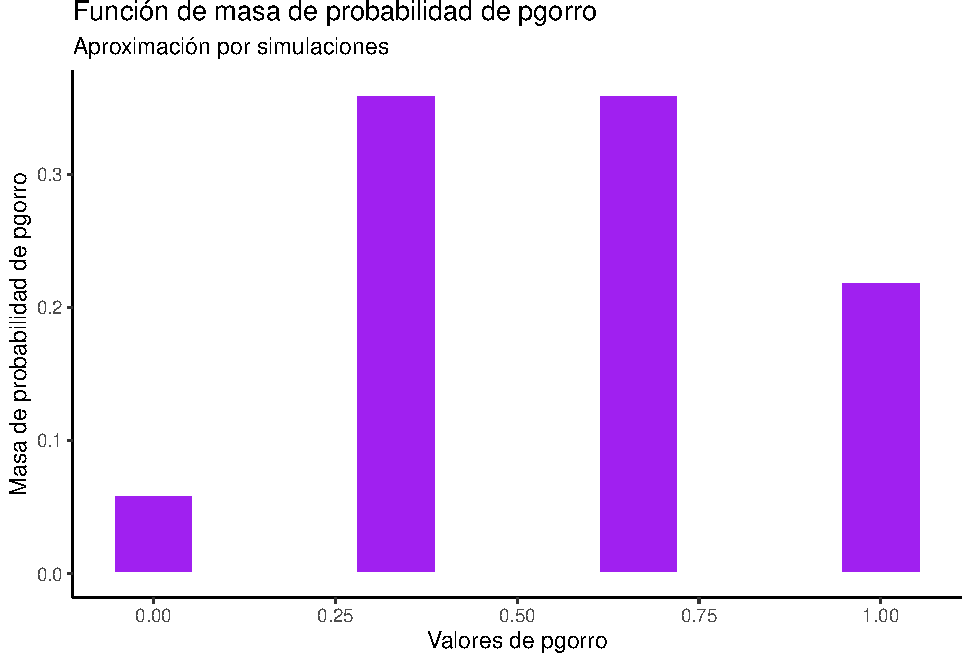
\includegraphics{InferenciaEstadistica_files/figure-latex/unnamed-chunk-18-1.pdf}

Esto implica que aunque tengamos datos fijos \(\{ R,R,R A, A\}\) como la extracción de la muestra es aleatoria el valor de \(\hat{p}\) va a variar por el simple proceso de selección aleatoria de la muestra. Darnos cuenta de qué tanto varía nuestro valor a estimar y cómo se aleja (o no) de la verdad va a ser un punto muy importante (en general queremos estimadores \(\hat{p}\) que no se alejen de los valores verdaderos).

Ahora, los estimadores \(\hat{p}\) no son únicos y se nos puede ocurrir otro estimador como ejemplo:

\hypertarget{estimador-de-muxe1xima-verosimilitud-maximizaciuxf3n-discreta}{%
\subsection{Estimador de máxima verosimilitud (maximización discreta)}\label{estimador-de-muxe1xima-verosimilitud-maximizaciuxf3n-discreta}}

Una segunda opción es buscar bajo qué valor de \(p\) (de muchos posibles) son más probables los datos observados. Este criterio se conoce como el criterio de \textbf{máxima verosimilitud}. La idea es ver, bajo cada una de las construcciones posibles de la caja (\emph{i.e.} \(\{ R, R, R, R, R\}\), \(\{ R, R, R, R, A\}\), \(\{ R, R, R, A, A\}\), \(\{ R, R, A, A, A\}\), \(\{ R, A, A, A, A\}\), \(\{ A, A, A, A, A\}\)) son más probables los datos observados \(( R, R, A)\) y elegir esa caja.
Vamos a resolver este problema calculando bajo cada escenario de caja las probabilidades de obtener la combinación observada \(( R, R, A)\).

La pregunta, antes de resolver el problema, es \emph{¿y esto para qué sirve?} . Si bien los ejercicios de pelotas de colores y cajas son divertidos, estos por sí mismos no llegan muy lejos. Lo importante es que los ejercicios de urnas \emph{son abstracciones} de problemas reales. Por ejemplo, el problema de urnas ocurre de manera poblacional cuando nos interesa estimar una proporción. En un país hay personas que padecen diabetes R y sin diabetes A. Se sabe que en el país hay 100 millones de personas. La proporción exacta (dentro del país) es desconocida. Sin embargo podemos hacer una encuesta y obtener una muestra de 100 personas dentro de las cuáles 20 padecieron diabetes y 80 no (\(\{20 R, 80 A\}\)). De aquí, usando el mismo razonamiento que usaremos con la caja de pelotas podemos buscar la combinación de personas con diabetes y sin diabetes en el país donde la combinación de \(\{20 R, 80 A\}\) es la más probable.

Este mismo razonamiento puede cambiarse de múltiples formas. En una encuesta podemos tener más de dos opciones. Por ejemplo, si interesa determinar la cantidad de personas que votarían por el partido rojo \(R\), por el azul \(A\) o por el negro \(B\) el modelo de pelotas en una caja ahora tiene tres tipos de pelota (y si hay \(n\) partidos habría \(n\) colores). Puede que los colores estén relacionados entre sí y extraer uno garantice la extracción de otro (por ejemplo si se entrevista gente en casas es muy probable que si se vive un niño en una casa \emph{a fuerza} viva un adulto en ella mientras que la relación inversa no funciona: que un adulto habite una casa no determina que viva un niño en la misma). Otros cambios posibles son en el mecanismo de selección. Pudiera ser que las pelotas rojas \(R\) fueran más grandes que las azules \(A\) de tal forma que cuando se extrajeran hubiera mayor probabilidad de tener rojas en la muestra. Esto pasa, por ejemplo, cuando se hacen encuestas de productos. Generalmente sólo aquellas personas que tienen un sentimiento muy fuerte hacia un producto contestan la encuesta. De ahí que haya muchísimas reseñas diciendo que los productos son malísimos o buenísimos y nada intermedio: la gente que reseña algo con 3 estrellas son las pelotas azules que son más difíciles de extraer. Poco a poco veremos otros problemas con pelotas y urnas con sus análogos al mundo real. Por ahora resolvamos el que se especifica más arriba.

\hypertarget{ejemplo-5-muestreo-de-urna-con-dos-clases-con-orden-con-reemplazo}{%
\subsection{Ejemplo 5: Muestreo de urna con dos clases, con orden, con reemplazo}\label{ejemplo-5-muestreo-de-urna-con-dos-clases-con-orden-con-reemplazo}}

Considera una urna con cinco pelotas de colores rojo \(R\) y azul \(A\). Se desconoce la proporción de pelotas en la urna. Las pelotas son indistinguibles entre sí salvo por el color. Se extrae de manera ordenada primero una bola roja, \(R\), y se devuelve a la urna. Luego se extrae una segunda bola roja, \(R\), y se devuelve a la urna. Finalmente se extrae una tercera bola y resulta azul: \(A\). La combinación ordenada de pelotas extraídas es: \(( R, R, A)\). Suponiendo todas las pelotas tienen la misma probabilidad de salir, cuál urna genera con mayor probabilidad los datos observados (y por tanto sería nuestra opción para decidir qué urna es la que tenemos): \(\{ R, R, R, R, R\}\), \(\{ R, R, R, R, A\}\), \(\{ R, R, R, A, A\}\), \(\{ R, R, A, A, A\}\), \(\{ R, A, A, A, A\}\) ó \(\{ A, A, A, A, A\}\).

\begin{quote}
\hypertarget{soluciuxf3n-5-muestreo-de-urna-con-dos-clases-con-orden-con-reemplazo}{%
\subsection{Solución 5: Muestreo de urna con dos clases, con orden, con reemplazo}\label{soluciuxf3n-5-muestreo-de-urna-con-dos-clases-con-orden-con-reemplazo}}

Hay dos combinaciones de posible urna que podemos descartar desde un inicio: la que sólo tiene rojos \(\{ R, R, R, R, R\}\) y la que sólo tiene azules \(\{ A, A, A, A, A\}\). Esto porque los datos observados nos muestran que obtuvimos tantos rojos como azules. En estas dos descartadas la probabilidad de obtener \(( R, R, A)\) es cero. Quedan como cajas posibles: la de cuatro rojas \(\{ R, R, R, R, A\}\), la de tres rojas \(\{ R, R, R, A, A\}\), la de tres azules \(\{ R, R, A, A, A\}\), la de una roja \(\{ R, A, A, A, A\}\). Comenzaré mi análisis con la primera que puse: los otros análisis son similares.

\textbf{Análisis de \(\{ R, R, R, R, A\}\)}

Una de las formas más posibles de enlistar todos los escenarios es con un árbol. La forma larga (e impráctica) consiste en enlistar cada una de las formas de extraer las pelotas de la urna como muestra la siguiente imagen:

\begin{figure}
\centering
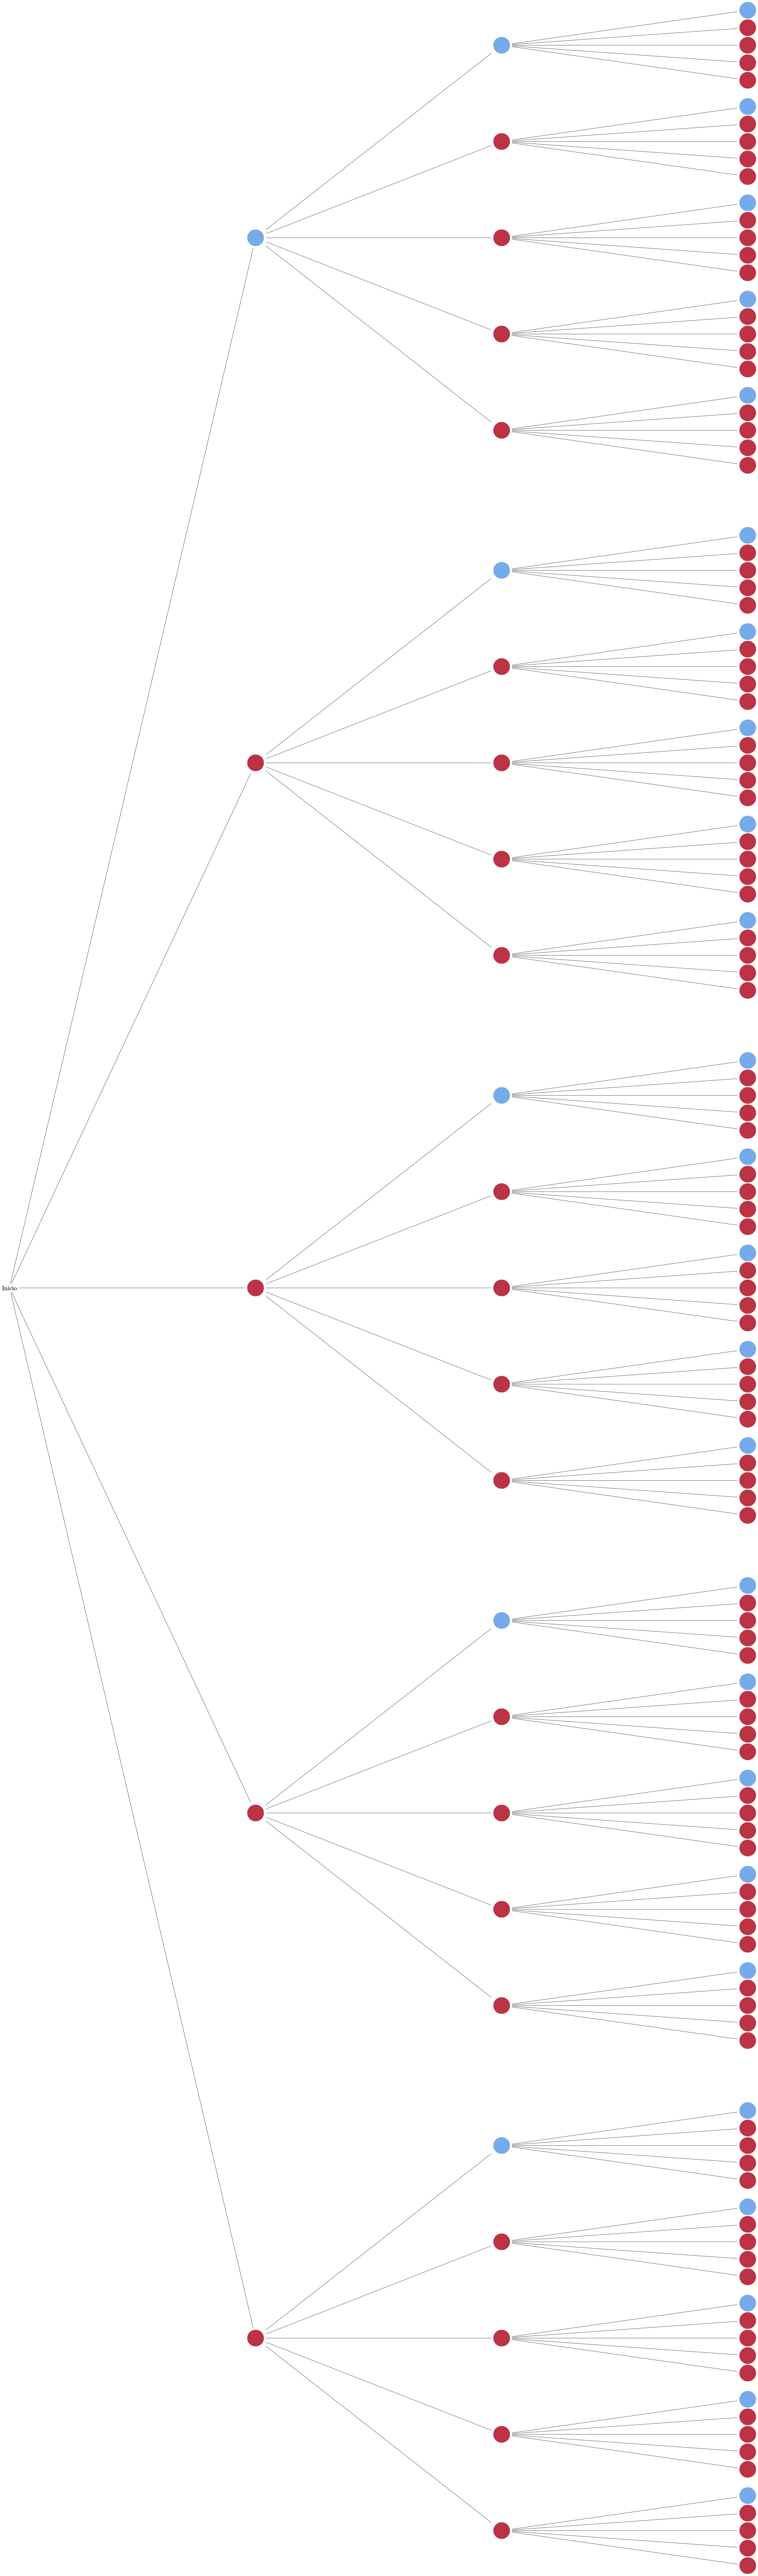
\includegraphics{./images/arbol_decision_1.jpeg}
\caption{Árbol de decisión para el análisis de \(\{ R, R, R, R, A\}\) con reemplazo}
\end{figure}

Esta es una forma ``segura'' de resolver un problema: puede ser largo pero si no se te olvida nada ¡siempre es una posibilidad! Observa que de todas las opciones (combinadas del primer nodo,el segundo y el tercero) se tienen 16 extracciones de la forma \(( R, R, A)\) de un total de 125 extracciones (\(5\) opciones en el último nodo por \(5\) formas de extraer el segundo por \(5\) opciones primeras dan 125). La probabilidad entonces de extraer \(( R, R, A)\) bajo este esquema es:
\[
\textrm{Probabilidad de ( R, R, A) dada la urna \{ R, R, R, R, A\} con reemplazo} =  \dfrac{16}{125} 
\]

\textbf{Análisis de \(\{ R, R, R, A, A\}\)}

Vale la pena para este segundo análisis podar un poco el árbol. Podemos darnos cuenta que en el caso anterior todas las ramas rojas son iguales por lo que quizá no vale la pena ponerlas todas. Al calcular la probabilidad de la extracción \(( R, R, A)\) dado que la urna es de la forma \(\{ R, R, R, A, A\}\) trabajaremos más a fondo el árbol. El árbol inicial es como sigue:

\begin{figure}
\centering
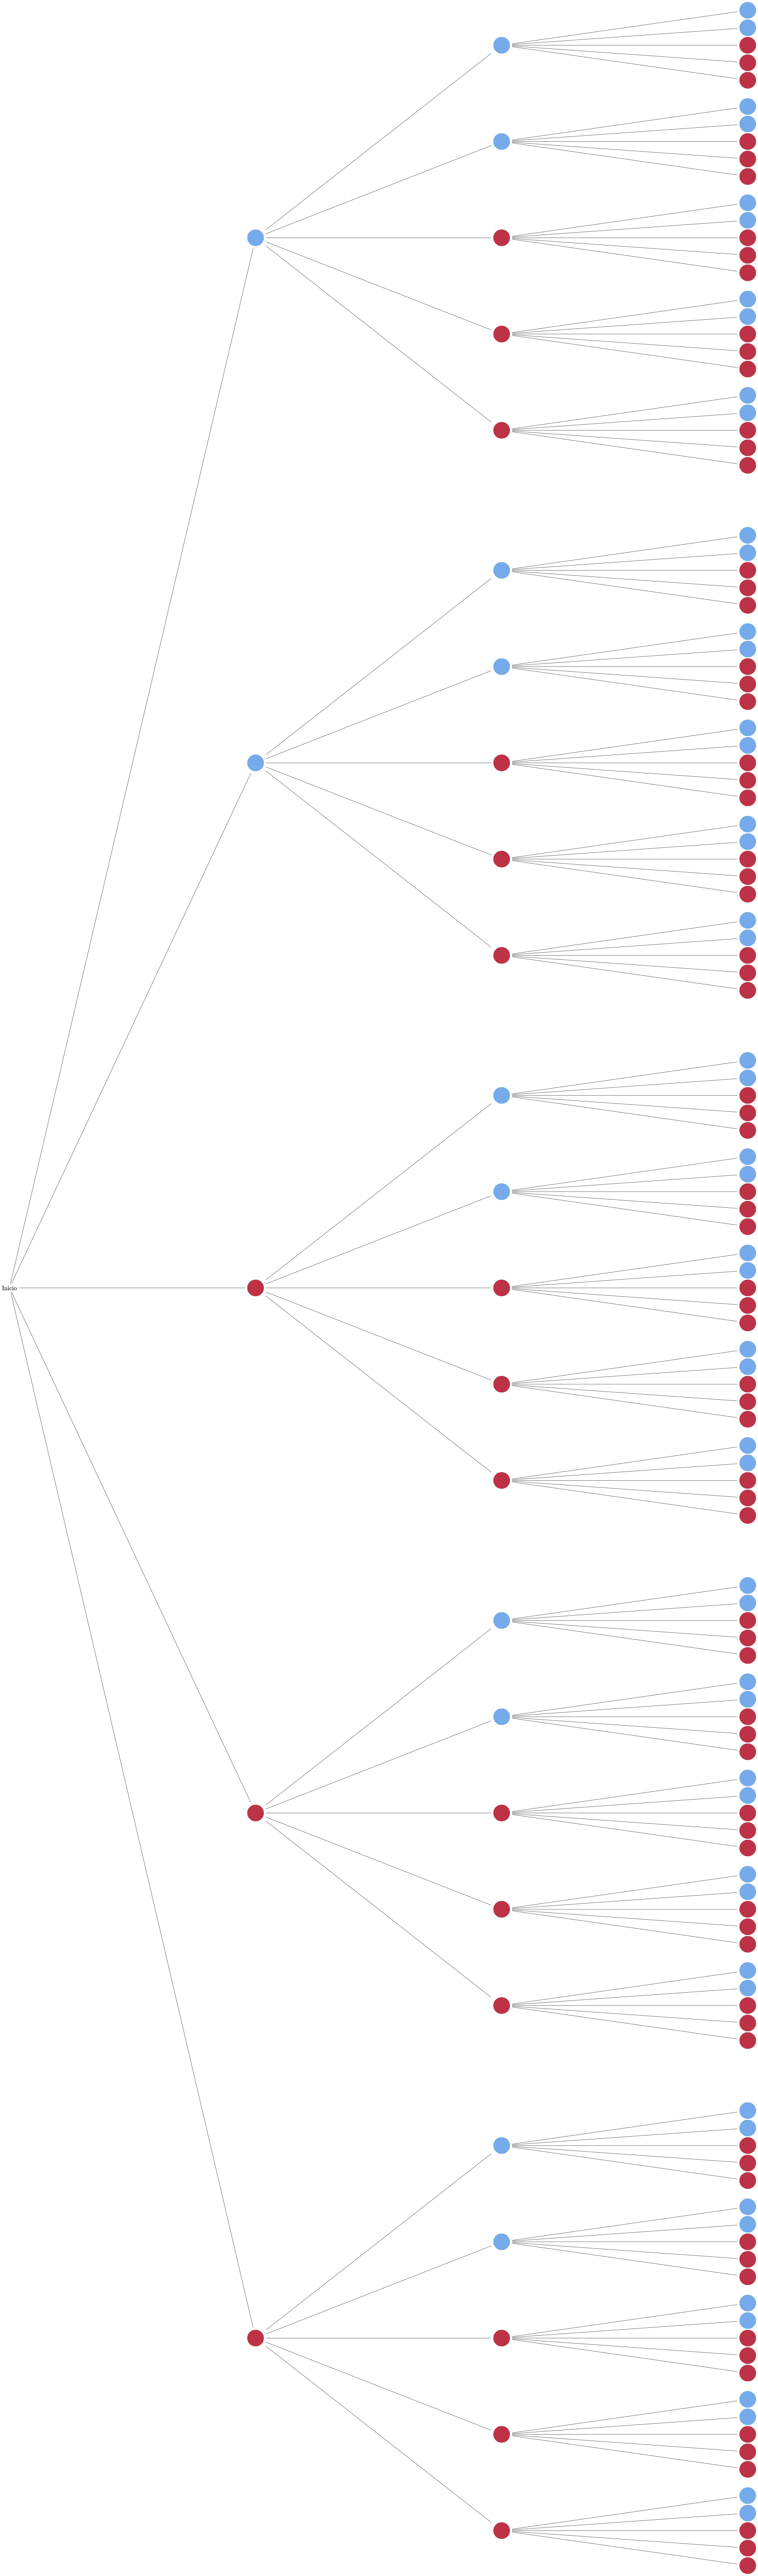
\includegraphics{./images/arbol_decision_2.jpeg}
\caption{Árbol de decisión en el caso \(\{ R, R, R, A, A\}\) con reemplazo}
\end{figure}

En este caso notamos que todos los caminos iniciados por rojo, R, son idénticos lo mismo que los caminos iniciados por azul A por lo que podemos simplificar el árbol copiando sólo las ramas distintas y anotando cada rama a cuántas representa (las azules son \(2\) de \(5\) mientras que las rojas \(3\) de \(5\) de ahí los números \(2/5\) y \(3/5\)).

\begin{figure}
\centering
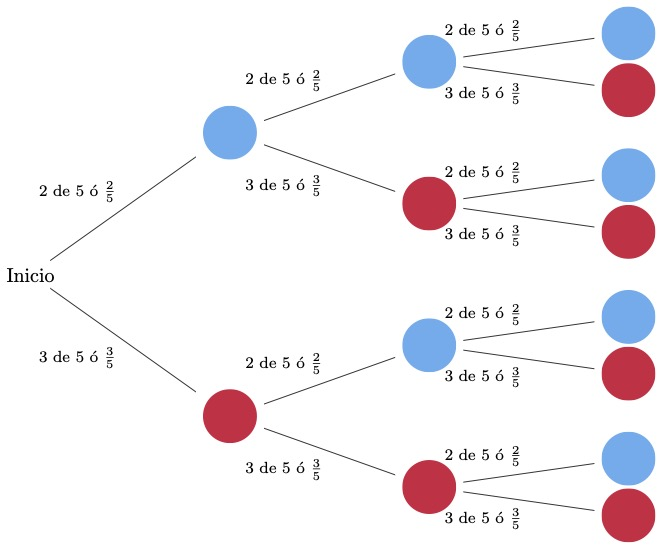
\includegraphics{./images/arbol_decision_2_1.jpeg}
\caption{Árbol de decisión simplificado para el análisis de \(\{ R, R, R, A, A\}\) con reemplazo}
\end{figure}

Para el caso que nos atañe en esta ocasión: obtener primero roja, luego otra roja y finalmente azul, \(( R, R, A)\), la única opción es la rama de abajo con probabilidades dadas por:
\[
\textrm{Probabilidad de ( R, R, A) dada la urna \{R, R, R, A, A\} con reemplazo}  = \dfrac{3 \times 3 \times 2}{5 \times 5 \times 5} = \dfrac{18}{125}
\]
Esta forma reducida es equivalente a la que hubiéramos obtenido haciendo el análisis completo del árbol (por la primera imagen donde hay \(18\) opciones de \(125\) resultados). El producto de arriba refiere a el número de opciones para primera roja, por el número de opciones para segunda roja \emph{dado} que la primera fue roja y la última son las opciones para una tercera azul \emph{condicional} en que las dos primeras fueron rojas. En el denominador sólo multiplicamos los casos totales que son \(5\) ramas iniciales que ramifican en \(5\) nodos secundarios y \(5\) hojas finales.

Tómate unos minutos para intentar justificar por qué este conteo de multiplicaciones es equivalente a haber contado todas. Asegúrate de entenderlo bien antes de continuar ¡volveremos a ello más adelante!

\textbf{Análisis de \(\{ R, R, A, A, A\}\)}

En este análisis usaremos el mismo truco de un árbol de decisiones reducido que usamos la vez pasada. Lo construiremos paso a paso para mostrar el proceso. De manera inicial tenemos dos opciones: roja (\(2\) bolas de \(5\)) ó azul (\(3\) bolas de \(5\)) por lo que a partir de la raíz construimos el árbol con las dos opciones y sus probabilidades

\begin{figure}
\centering
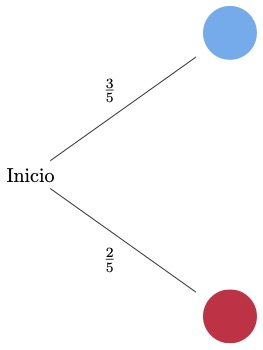
\includegraphics{./images/arbol_decision_3_1.jpeg}
\caption{Versión 1 del árbol de decisión simplificado para \(\{ R, R, A, A, A\}\) con reemplazo}
\end{figure}

Dentro de la rama azul de nuevo tenemos la posibilidad de extraer rojas (\(2\) de \(5\)) o azules (\(3\) de \(5\)) por lo que se acoplan a la rama:

\begin{figure}
\centering
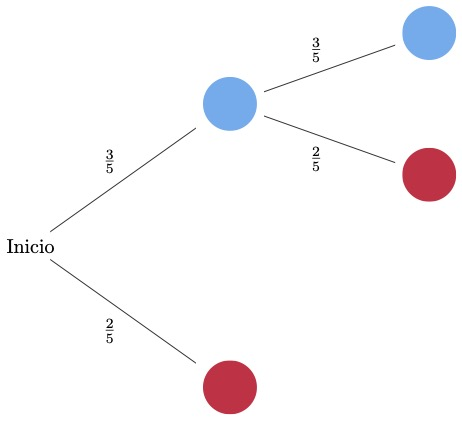
\includegraphics{./images/arbol_decision_3_2.jpeg}
\caption{Versión 2 del árbol de decisión simplificado para \(\{ R, R, A, A, A\}\) con reemplazo}
\end{figure}

La lógica es idéntica si salió roja: hay \(2/5\) de probabilidad de extraer una roja o \(3/5\) de extraer una azul

\begin{figure}
\centering
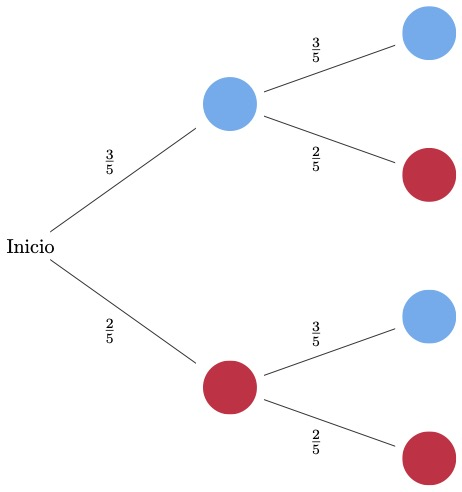
\includegraphics{./images/arbol_decision_3_3.jpeg}
\caption{Versión 3 del árbol de decisión simplificado para \(\{ R, R, A, A, A\}\) con reemplazo}
\end{figure}

Finalmente las últimas ramas del árbol se agregan de manera idéntica: \(2/5\) de rojas y \(3/5\) de azul en cada una de las posibles extracciones.

\begin{figure}
\centering
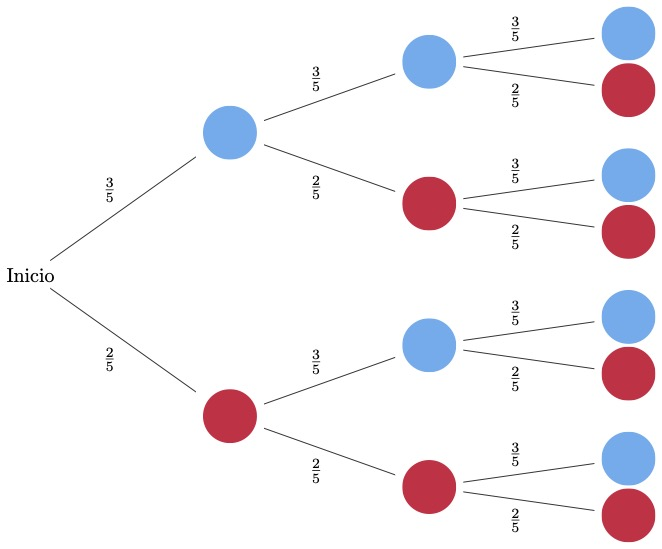
\includegraphics{./images/arbol_decision_3_4.jpeg}
\caption{Versión final del árbol de decisión simplificado para \(\{ R, R, A, A, A\}\) con reemplazo}
\end{figure}

Notamos entonces que podemos hacer el cálculo multiplicando (como hicimos la vez pasada) para obtener:
\[
\textrm{Probabilidad de ( R, R, A) dada la urna \{R, R, A, A, A\} con reemplazo}  = \dfrac{2}{5} \cdot \dfrac{2}{5} \cdot \dfrac{3}{5} = \dfrac{12}{125}
\]

\textbf{Análisis de \(\{ R, A, A, A, A\}\)}

Ya para este último caso los árboles de decisiones te son familiares por lo que puedes verificar que en este caso el árbol es el siguiente:

\begin{figure}
\centering
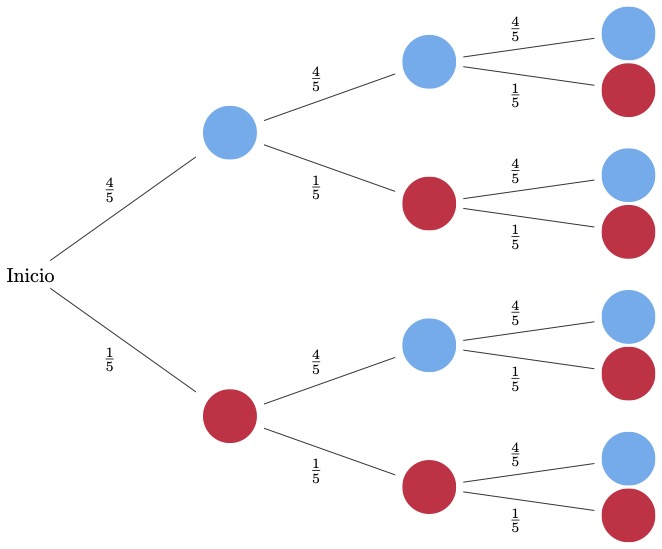
\includegraphics{./images/arbol_decision_4.jpeg}
\caption{Árbol de decisión simplificado para el análisis de \(\{ R, A, A, A, A\}\) con reemplazo}
\end{figure}

donde la probabilidad de \$( R, R, A) \$ dado que la urna es \(\{ R, A, A, A, A\}\) está dada por:
\[
\textrm{Probabilidad de ( R, R, A) dada la urna \{ R, A, A, A, A\} con reemplazo} = \dfrac{1}{5} \cdot \dfrac{1}{5} \cdot \dfrac{4}{5} = \dfrac{4}{125}.
\]

\textbf{Conclusión}

Después de que analizamos las probabilidades bajo todas las combinaciones posibles de urna concluimos que la que tiene probabilidad más alta de generar en ese orden rojo, luego rojo y finalmente azul, \(( R, R, A)\), es la urna \(\{R, R, R, A, A\}\) pues si la urna tiene esa combinación de pelotas la probabilidad de extraer \(( R, R, A)\) es:
\[
\textrm{Probabilidad de ( R, R, A) dada la urna \{R, R, R, A, A\} con reemplazo} = \dfrac{18}{125} = 0.144.
\]
Siguiendo la idea de que la urna que tenemos es la que tiene mayor probabilidad de generar los datos observados (esto se conoce como \emph{criterio de máxima verosimilitud} en estadística) entonces estimaríamos que la urna que tenemos es \(\{R, R, R, A, A\}\) por lo que \(\hat{p} = \frac{3}{5}\) es el estimador de máxima verosimilitud de \(p\).

\textbf{OJO} Dadas las observaciones \(( R, R, A)\) no podemos determinar a ciencia cierta cuál es la combinación de pelotas en la urna que tenemos. Por lo que siempre puede pasar que la combinación \emph{real} sea distinta. Aquí el modelo nos dice por cuál optar (de manera lógica, aquella que genera con mayor probabilidad lo que observamos) pero la realidad ¡puede estar por otro lado!
\end{quote}

Una vez que obtuvimos el estimador, \(\hat{p}\), la segunda pregunta que nos interesará resolver es \emph{qué tan buen estimador es \(\hat{p}\)}. Para ello también buscaríamos describir su distribución probabilística (su masa, su varianza, su valor esperado). Esto lo dejaremos para más adelante.

\hypertarget{resumen-de-la-secciuxf3n}{%
\section{Resumen de la sección}\label{resumen-de-la-secciuxf3n}}

En esta sección aprendimos que, en el mundo de las ideas, tenemos poblaciones de las cuales obtenemos subconjuntos (muestras). Las muestras observadas corresponden a los datos mientras que las muestras (sin el ``observadas'') corresponden al modelo en el mundo de las ideas. Lo que buscamos es estimar los valores que necesitamos para determinar el modelo (parámetros) y esos valores se obtienen a través de estimadores (puede haber varios para el mismo parámetro). Los estimadores viven también en el mundo de los modelos y ahí tienen su distribución de probabilidad, sus masas y densidades, sus valores esperados y sus varianzas. Describir esto nos ayuda a saber cómo se comportan los estimadores y decidir cuáles son los buenos. Profundizaremos más en la siguiente sección donde haremos un ejemplo muy específico: ¿qué pasa si mi población está compuesta de variables aleatorias normales? Jugaremos con ello y veremos por qué es normal usar la normal.

\hypertarget{R}{%
\chapter{R}\label{R}}

\hypertarget{programaciuxf3n-en-r}{%
\section{\texorpdfstring{Programación en \texttt{R}}{Programación en R}}\label{programaciuxf3n-en-r}}

\begin{figure}

{\centering 
\includegraphics[width=17.78in]{images/rlogo} 

}

\caption{`R` es un programa chido de estadística. FIN.}\label{fig:unnamed-chunk-20}
\end{figure}

Una de las primeras cosas que necesitamos saber es que \texttt{R} (por más que sus más ávidos defensores digan lo contrario) no es para todo. Si tú ya conoces otro lenguaje (sea \texttt{Stata}, \texttt{Excel}, \texttt{SAS}, \texttt{Python}, \texttt{Matlab}, \texttt{Julia}, etc) sabrás utilizar muchas de sus opciones. Estoy seguro que, de conocer uno de estos, te será muchísimo más fácil seguir sacando promedios en tu lenguaje favorito que en \texttt{R}, realizar regresiones lineales es probablemente más sencillo en \texttt{Stata} mientras que las gráficas de barras para mí son más simples en \texttt{Excel}, \texttt{Python} excede en aplicaciones de inteligencia artificial mientras que \texttt{Matlab} es más veloz que \texttt{R}, \texttt{Julia} tiene muchas cosas de ecuaciones diferenciales que nadie más.

Lo que probablemente no sea más sencillo de hacer en otro lenguaje es realizar análisis estadístico, gráficas de todo tipo y modelos de simulación. Para eso, \texttt{R} es, indiscutiblemente, una de las mejores opciones para quienes no conocen de programación\footnote{Modelos de simulación más avanzados suelen hacerse en \texttt{C}, \texttt{C++} o \texttt{Fortran} por su velocidad; empero, es necesario conocer más de programación.}.

Finalmente, uno de los consejos más importantes que te puedo dar es que este curso no te va a servir si no practicas. Igual que como pasa con los idiomas uno no aprende \texttt{R} en una semana \emph{sin practicarlo después}. Mi sugerencia es que, a la vez que sigues estas notas comiences a trabajar un proyecto \emph{tuyo} específico junto con \href{https://yandex.com}{el buscador de Internet de tu preferencia} a la mano y empieces a usar \texttt{R} en él. Practica\footnote{La práctica hace al maestro}.

\hypertarget{puntos-a-favor-de-r}{%
\subsection{\texorpdfstring{Puntos a favor de \texttt{R}}{Puntos a favor de R}}\label{puntos-a-favor-de-r}}

\begin{itemize}
\item
  Todo el mundo lo usa. Quizá éste es el punto más a favor. Si mucha gente lo conoce y lo utiliza, hay más opciones de ayuda. Los sitios de StackOverflow \href{https://stackoverflow.com}{en inglés} y \href{https://es.stackoverflow.com}{en español} son excelentes para pedir apoyo en \texttt{R}; los \href{https://groups.google.com/forum/\#!forum/r-help-archive}{grupos de usuarios de Google} son otra fuente muy buena. Entre más gente usa el programa; es más fácil obtener ayuda porque seguro alguien más tuvo hace ya tiempo el mismo problema que tú.
\item
  Todas las personas que trabajan en estadística publican sus métodos y su código en \texttt{R} (eso, claro, cuando publican sus métodos). Es raro encontrar \emph{un nuevo método estadístico} en el mundo y que no se pueda usar, de alguna forma, en \texttt{R}.
\item
  Dentro de los lenguajes de programación \texttt{R} es de los más sencillos. Quienes lo hicieron realmente se preocuparon por su público (de no especialistas) y en general desarrollan para él.
\item
  \texttt{R} es gratis. Y en esta época de austeridad, cualquier ahorro es bueno. Que sea gratis no significa que no esté respaldado: existen versiones de \texttt{R} respaldadas por grandes compañías como \href{https://mran.microsoft.com/open}{Microsoft}
\item
  Todo lo que se hace en \texttt{R} es público. \texttt{R} no tiene métodos secretos ni es una caja negra. Todo lo que hace cada una de las funciones de \texttt{R}, cualquiera lo puede revisar, por completo.
\item
  En \texttt{R} puedes hacer libros o notas ¡como este! donde guardes todo tu trabajo, reportes automatizados e incluso \href{https://gallery.shinyapps.io/086-bus-dashboard/}{documentos interactivos} para facilitar el análisis de datos.
\item
  \texttt{R} puede hacer gráficas bonitas:
\end{itemize}

\begin{center}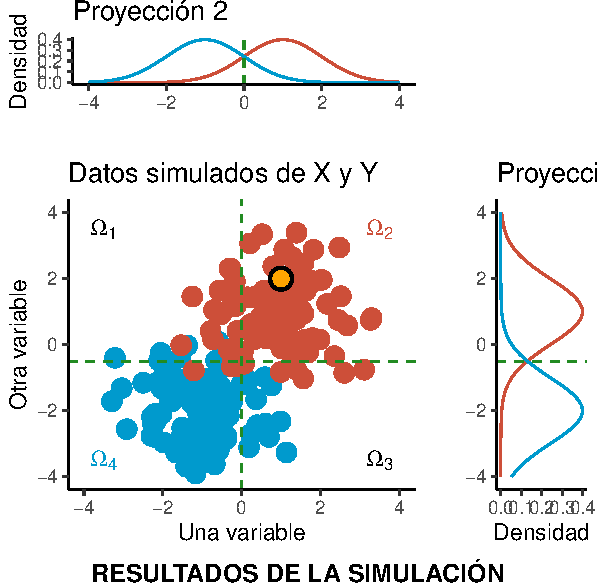
\includegraphics{InferenciaEstadistica_files/figure-latex/unnamed-chunk-21-1} \end{center}

Por supuesto, no todo es miel sobre hojuelas con \texttt{R}. Particularmente, algunos de los problemas con el lenguaje:

\begin{figure}

{\centering 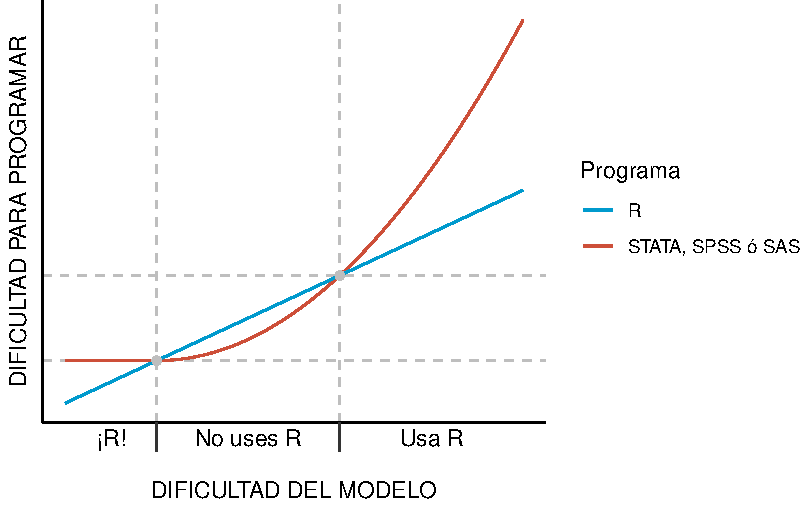
\includegraphics{InferenciaEstadistica_files/figure-latex/unnamed-chunk-22-1} 

}

\caption{La curva de aprendizaje de `R` es más empinada pero después de un rato vale la pena}\label{fig:unnamed-chunk-22}
\end{figure}

\begin{itemize}
\item
  La curva de aprendizaje es mucho más empinada que para otros programas estadísticos (como \texttt{Stata}, \texttt{SAS} o \texttt{SPSS}) ¡particularmente si es tu primera vez programando!
\item
  La mayor parte de las personas que trabajan en \texttt{R} no son programadores de verdad. Gran parte del código que te puedes encontrar \textbf{en el mundo real} está escrito \href{https://nsaunders.wordpress.com/2014/05/14/this-is-why-code-written-by-scientists-gets-ugly/}{con prisa para salir del aprieto} sin mucha planeación, con pocos comentarios, falta de control de versiones y pocas herramientas de revisión. ¡Internet está lleno de \href{https://codegolf.stackexchange.com/a/4011}{creaturas espantosas escritas en \texttt{R}}!
\end{itemize}

\begin{figure}

{\centering 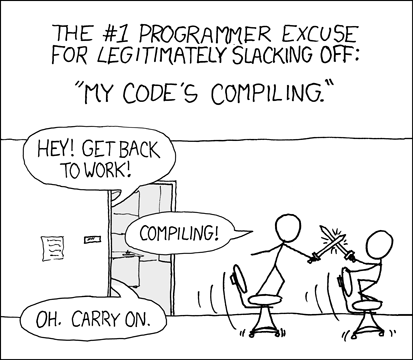
\includegraphics[width=5.74in]{images/compiling} 

}

\caption{`R` puede ser muy lento pero eso te da oportunidad de hacer otras cosas ;) .}\label{fig:unnamed-chunk-23}
\end{figure}

\begin{itemize}
\tightlist
\item
  \texttt{R} \href{https://github.com/matthieugomez/benchmark-stata-r}{de ninguna manera es veloz} por lo que algunos programas (lo veremos en simulación) pueden ser extremada (y dolorosamente) lentos.
\end{itemize}

\hypertarget{bienvenidx-a-r-bunny-wunnies-freak-out-suxed-asuxed-se-llama-esta-versiuxf3n}{%
\subsection{\texorpdfstring{Bienvenidx a \texttt{R}, Bunny-Wunnies Freak Out (sí, así se llama esta versión)}{Bienvenidx a R, Bunny-Wunnies Freak Out (sí, así se llama esta versión)}}\label{bienvenidx-a-r-bunny-wunnies-freak-out-suxed-asuxed-se-llama-esta-versiuxf3n}}

\texttt{R} es un lenguaje de cómputo y un programa estadístico \href{https://www.gnu.org/philosophy/free-sw.html}{libre}, gratuito, \href{http://adv-r.had.co.nz/Functional-programming.html}{de programación funcional} (¿qué es eso?), \href{https://en.wikipedia.org/wiki/Object-oriented_programming}{orientado a objetos} (\emph{what??}) que mutó a partir de otros dos lenguajes conocidos como \texttt{Scheme} y \texttt{S}\footnote{De ahí que se llame \texttt{R} porque la \texttt{R} es una mejor letra que la \texttt{S} (todos lo sabemos)
  -Atte. Rodrigo, el autor de este documento.}. El primero de estos fue desarrollado en el MIT por Sussman y Steele mientras que el segundo surgió en los laboratorios Bell\footnote{Mejor conocidos ahora como AT\&T, la compañía celular que nunca tiene señal.} creado por Becker, Wilks y Chambers. \texttt{R} \href{https://cran.r-project.org/doc/html/interface98-paper/paper_2.html}{nació en junio de 1995} a partir del trabajo de Ross Ihaka y Robert Gentleman\footnote{Sus nombres empiezan con la letra \texttt{R} ¿coincidencia?}.

Desde su creación, la mayor parte del desarrollo de \texttt{R} ha sido trabajo completamente voluntario de la \href{https://www.r-project.org/foundation/}{Fundación R}, del equipo de R Core y de miles de usuarios que han creado funciones específicas para \texttt{R} conocidas como paquetes (\texttt{packages}). Actualmente el repositorio más importante de \texttt{R}, CRAN, contiene más de \emph{16000} paquetes con distintas funciones para hacer ¡lo que quieras!

Como todo el trabajo en \texttt{R} es voluntario hace falta:

\begin{enumerate}
\def\labelenumi{\arabic{enumi}.}
\item
  Una homologación en los métodos. Puedes encontrar varias funciones \emph{que supuestamente hacen exactamente lo mismo} (como es el caso de \texttt{emojifont}, \texttt{fontemoji} y \texttt{emoGG} para graficar usando emojis).
\item
  Estandarizar la notación. Algunos paquetes como aquellos del \texttt{tidyverse} (veremos más adeltna) utilizan \texttt{pipes} (\texttt{\%\textgreater{}\%}); estos sólo funcionan en el \texttt{tidyverse} pero no fuera del mismo.
\end{enumerate}

Sin embargo, también es una gran ventaja que sean los usuarios de \texttt{R} quienes guían su desarrollo. El lenguaje va mutando según peticiones de las personas que lo usan. Si hay algo que te gustaría \texttt{R} tuviera y aún no existe ¡lo puedes proponer!

\hypertarget{instalando-cosas}{%
\section{Instalando cosas}\label{instalando-cosas}}

\hypertarget{instalaciuxf3n-de-r}{%
\subsection{\texorpdfstring{Instalación de \texttt{R}}{Instalación de R}}\label{instalaciuxf3n-de-r}}

\begin{figure}

{\centering 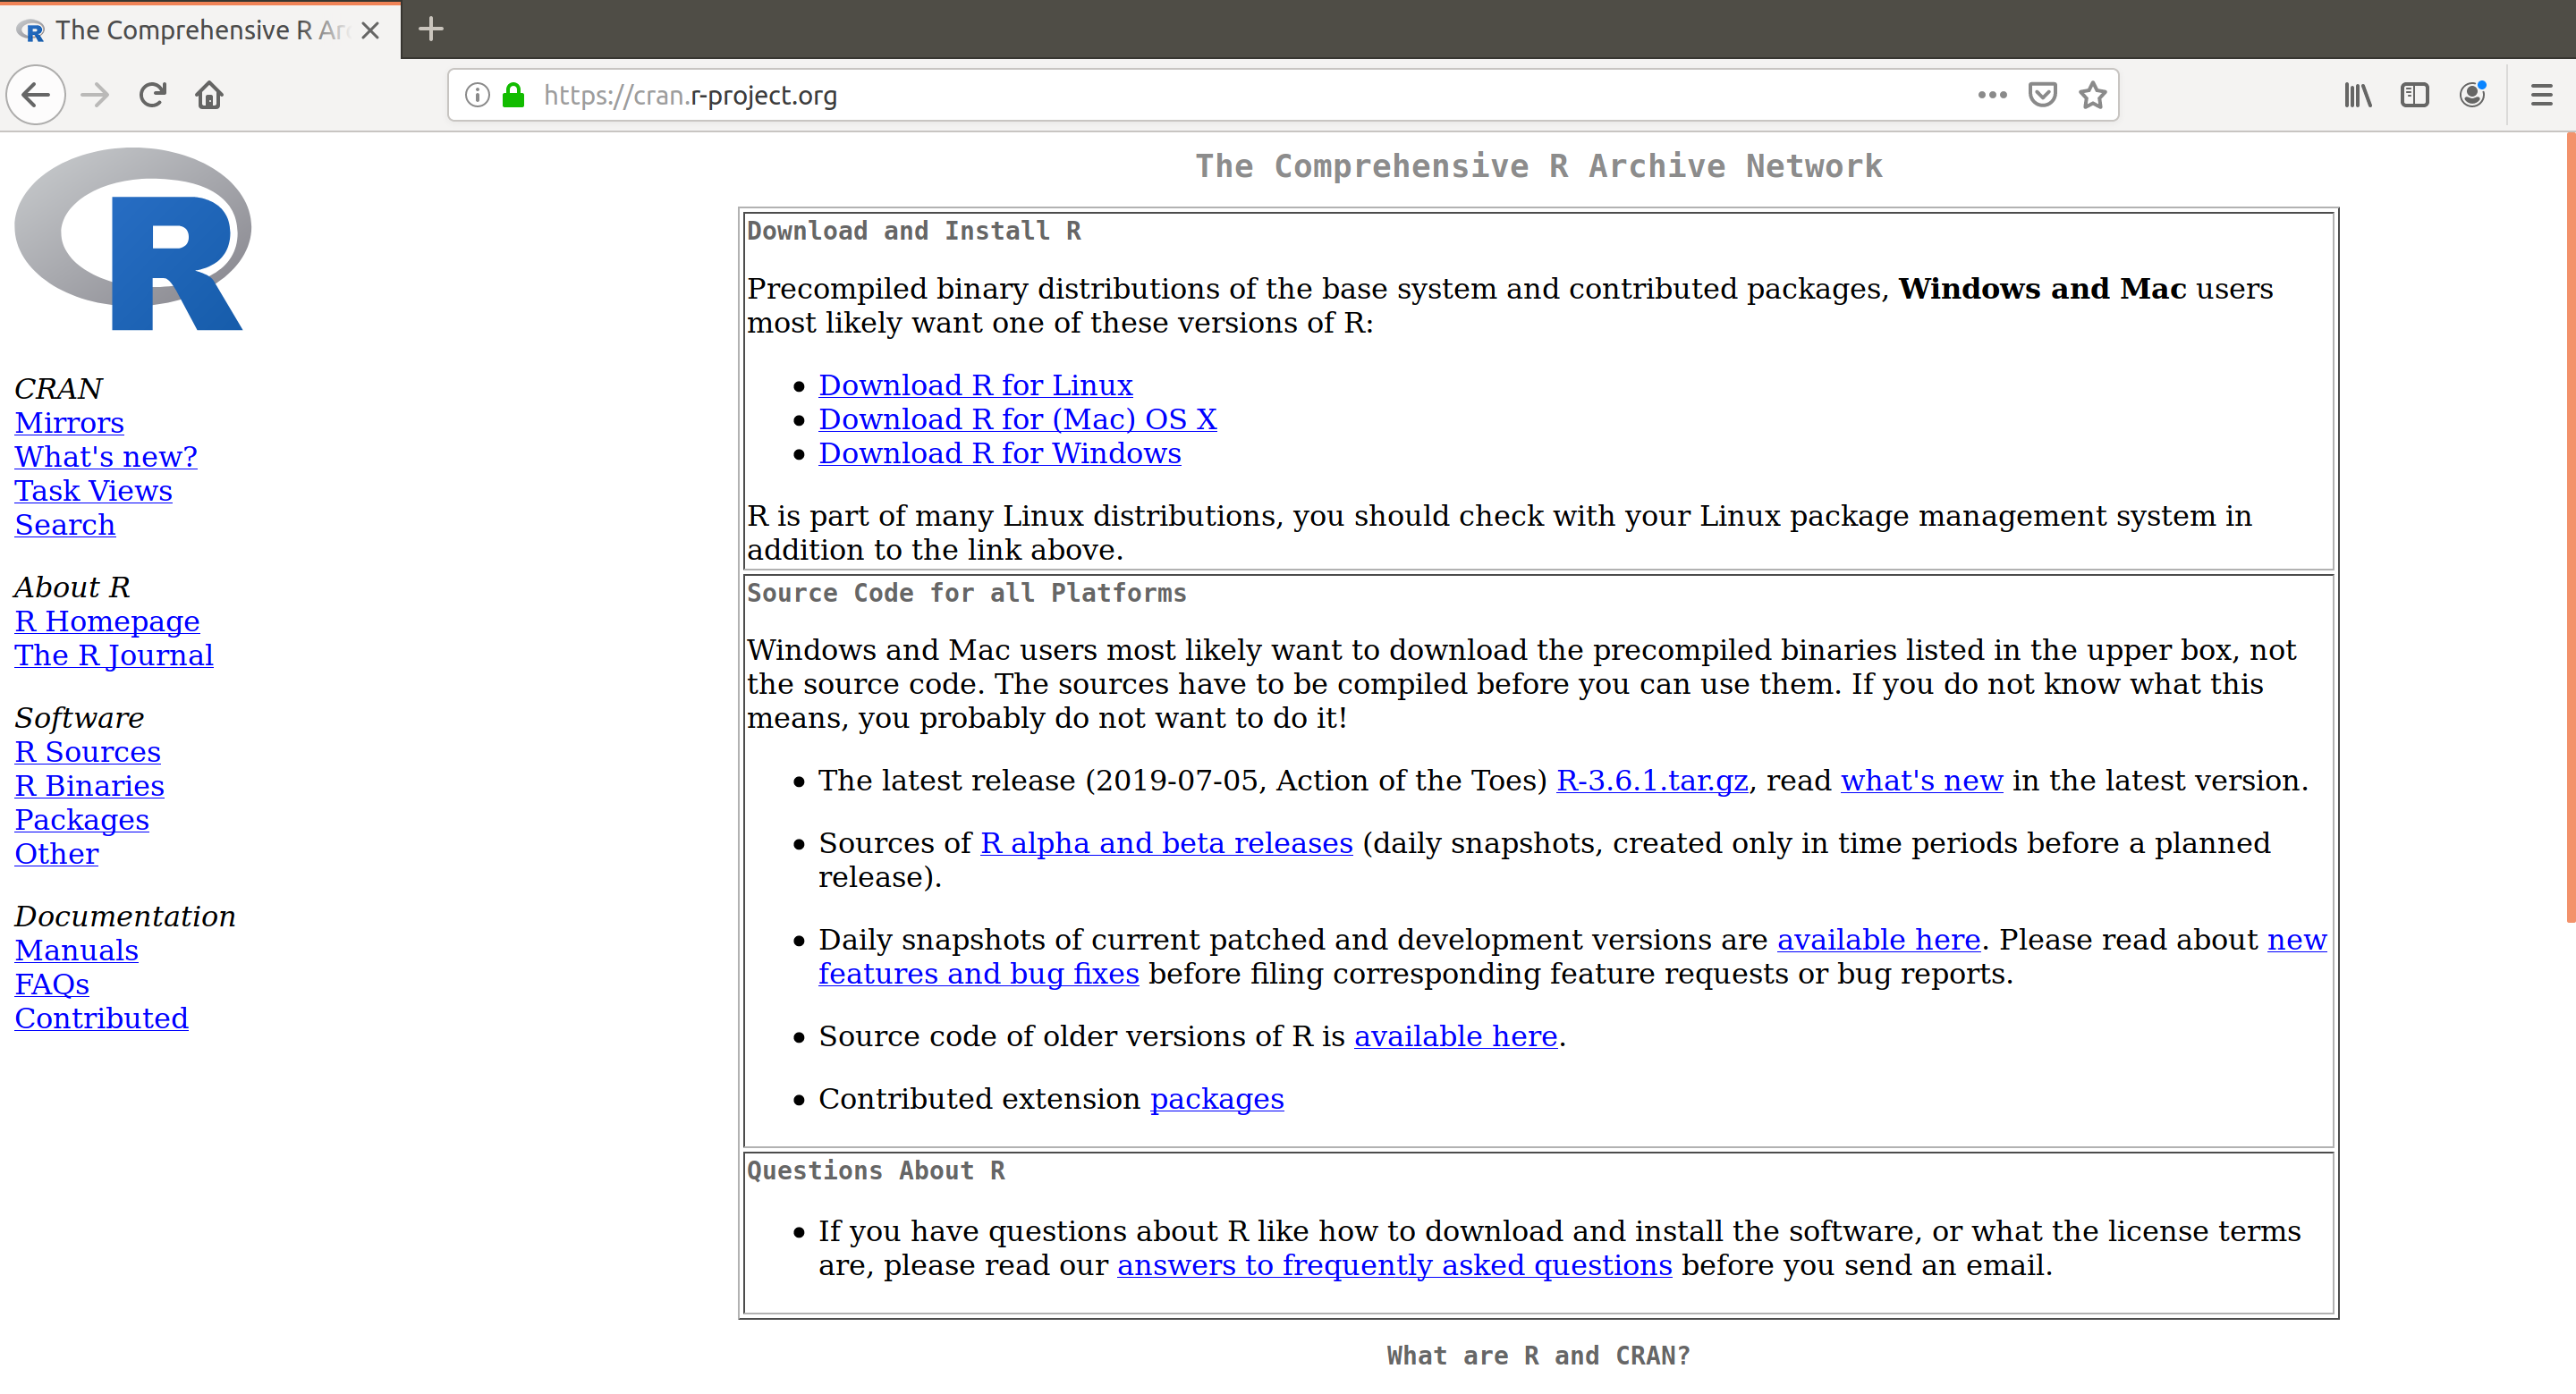
\includegraphics[width=40in]{images/CRAN1} 

}

\caption{Oficialmente, la página de `R` es de las páginas más feas del mundo. ¡No te dejes llevar por las apariencias!}\label{fig:unnamed-chunk-24}
\end{figure}

A lo largo de estas notas estaré trabajando con: R version 4.0.3 (2020-10-10) \emph{Bunny-Wunnies Freak Out}. La más reciente versión de \texttt{R} la puedes encontrar en \href{https://cran.r-project.org}{CRAN}. Para ello ve al sitio y selecciona tu plataforma.

\begin{quote}
\textbf{Nota usuarios de Mac} En algunas Mac, al abir R, aparece el siguiente mensaje de advertencia:
\texttt{During\ startup\ -\ Warning\ messages:\ 1:\ Setting\ LC\_CTYPE\ failed\ {[}...{]}}
para \href{https://stackoverflow.com/questions/9689104/installing-r-on-mac-warning-messages-setting-lc-ctype-failed-using-c}{solucionarlo} ve a \texttt{Aplicaciones} y abre \texttt{Terminal}. Copia y pega en ella el siguiente texto:
\texttt{defaults\ write\ org.R-project.R\ force.LANG\ en\_US.UTF-8}
Da enter, cierra la \texttt{Terminal} y reinicia \texttt{R}.
\end{quote}

\begin{itemize}
\tightlist
\item
  En el caso de Windows da clic en \texttt{Download\ R\ for\ Windows} y luego en \texttt{install\ R\ for\ the\ first\ time}. Finalmente, ejecuta el instalable que aparece al dar click en \texttt{Download\ R\ 4.0.3\ for\ Windows} .
\end{itemize}

\begin{quote}
Para este curso pudiera ser que requirieras las herramientas de desarrollador \href{https://cran.r-project.org/bin/windows/Rtools/}{Rtools}.
\end{quote}

\begin{itemize}
\item
  En el caso de Mac selecciona \texttt{Download\ R\ for\ (Mac)\ OS\ X} y luego elige \texttt{R-4.0.3.pkg}. En Mac puede que necesites instalar adicionalmente \href{https://www.xquartz.org}{XQuartz} (según tu versión de Mac). Si tu Mac es una versión suficientemente antigua, sigue las instrucciones específicas de \texttt{CRAN}.
\item
  En el caso de Linux al elegir \texttt{Download\ R\ for\ Linux} tendrás la opción de buscar tu distribución específica. Al elegirla, aparecerán instrucciones para tu terminal de comandos; síguelas. En el caso de Linux, según los paquetes de \texttt{R} que elijamos instalar en la computadora requerirás instalar paquetería adicional para tu distribución de Linux. \texttt{R} te informará de la paquetería necesaria conforme la requiera.
\end{itemize}

\begin{quote}
Si tienes problemas para instalar puedes usar \href{https://rstudio.cloud}{RStudio Cloud}.
\end{quote}

\hypertarget{instalaciuxf3n-de-rstudio}{%
\section{\texorpdfstring{Instalación de \texttt{RStudio}}{Instalación de RStudio}}\label{instalaciuxf3n-de-rstudio}}

\begin{figure}

{\centering 
\includegraphics[width=49.08in]{images/rstudio} 

}

\caption{RStudio es una empresa que se dedica a hacer cosas para R.}\label{fig:unnamed-chunk-25}
\end{figure}

\texttt{RStudio} es una interfaz gráfica (IDE) para \texttt{R}. Puedes pensar a \texttt{R} como el \emph{Bloc de Notas} y a \texttt{RStudio} como \emph{Word}. El \emph{Bloc} tiene todas las capacidades que necesitas para poder escribir; empero, es muchísimo mejor trabajar tus \emph{papers} en \emph{Word}. De la misma manera, \texttt{R} tiene todas las capacidades para hacer estadística \emph{pero un formato horrible} y \texttt{RStudio} se ha convertido en la más popular forma de usar \texttt{R}. Por supuesto que no es la única; algunas alternativas son \href{https://atom.io/packages/ide-r}{Atom con ide-r}, \href{https://marketplace.eclipse.org/content/statet-r}{Eclipse con StatET} y \href{https://rkward.kde.org}{RKWard}. En general es posible seguir estas notas sin que tengas \texttt{RStudio} pero, si es tu primera vez programando, no lo recomiendo.

\begin{quote}
Si ya tienes experiencia con lenguajes como Python, Javascript, Java ó alguno de los mil C que existen, no tendrás ningún problema usando el editor de tu preferencia.
\end{quote}

Para descargar \texttt{RStudio} ve a \href{https://www.rstudio.com}{su página} y da clic en \texttt{Download\ RStudio}. Baja tu pantalla hasta donde dice \texttt{Installers\ for\ Supported\ Platforms} y elige tu plataforma: \texttt{Windows}, \texttt{Mac\ OS\ X} ó tu sabor de \texttt{Linux} preferido. Una vez descargado el archivo, ábrelo y sigue las instrucciones que aparecen en pantalla.

\hypertarget{primeros-pasos-en-r-usando-rstudio}{%
\section{\texorpdfstring{Primeros pasos en \texttt{R} usando \texttt{RStudio}}{Primeros pasos en R usando RStudio}}\label{primeros-pasos-en-r-usando-rstudio}}

Una vez hayas instalado \texttt{R} y \texttt{RStudio}, abre \texttt{RStudio}\footnote{Si decidiste no instalar RStudio salta al final de esta sección.}. Te enfrentarás a una pantalla similar a esta:

\begin{figure}

{\centering 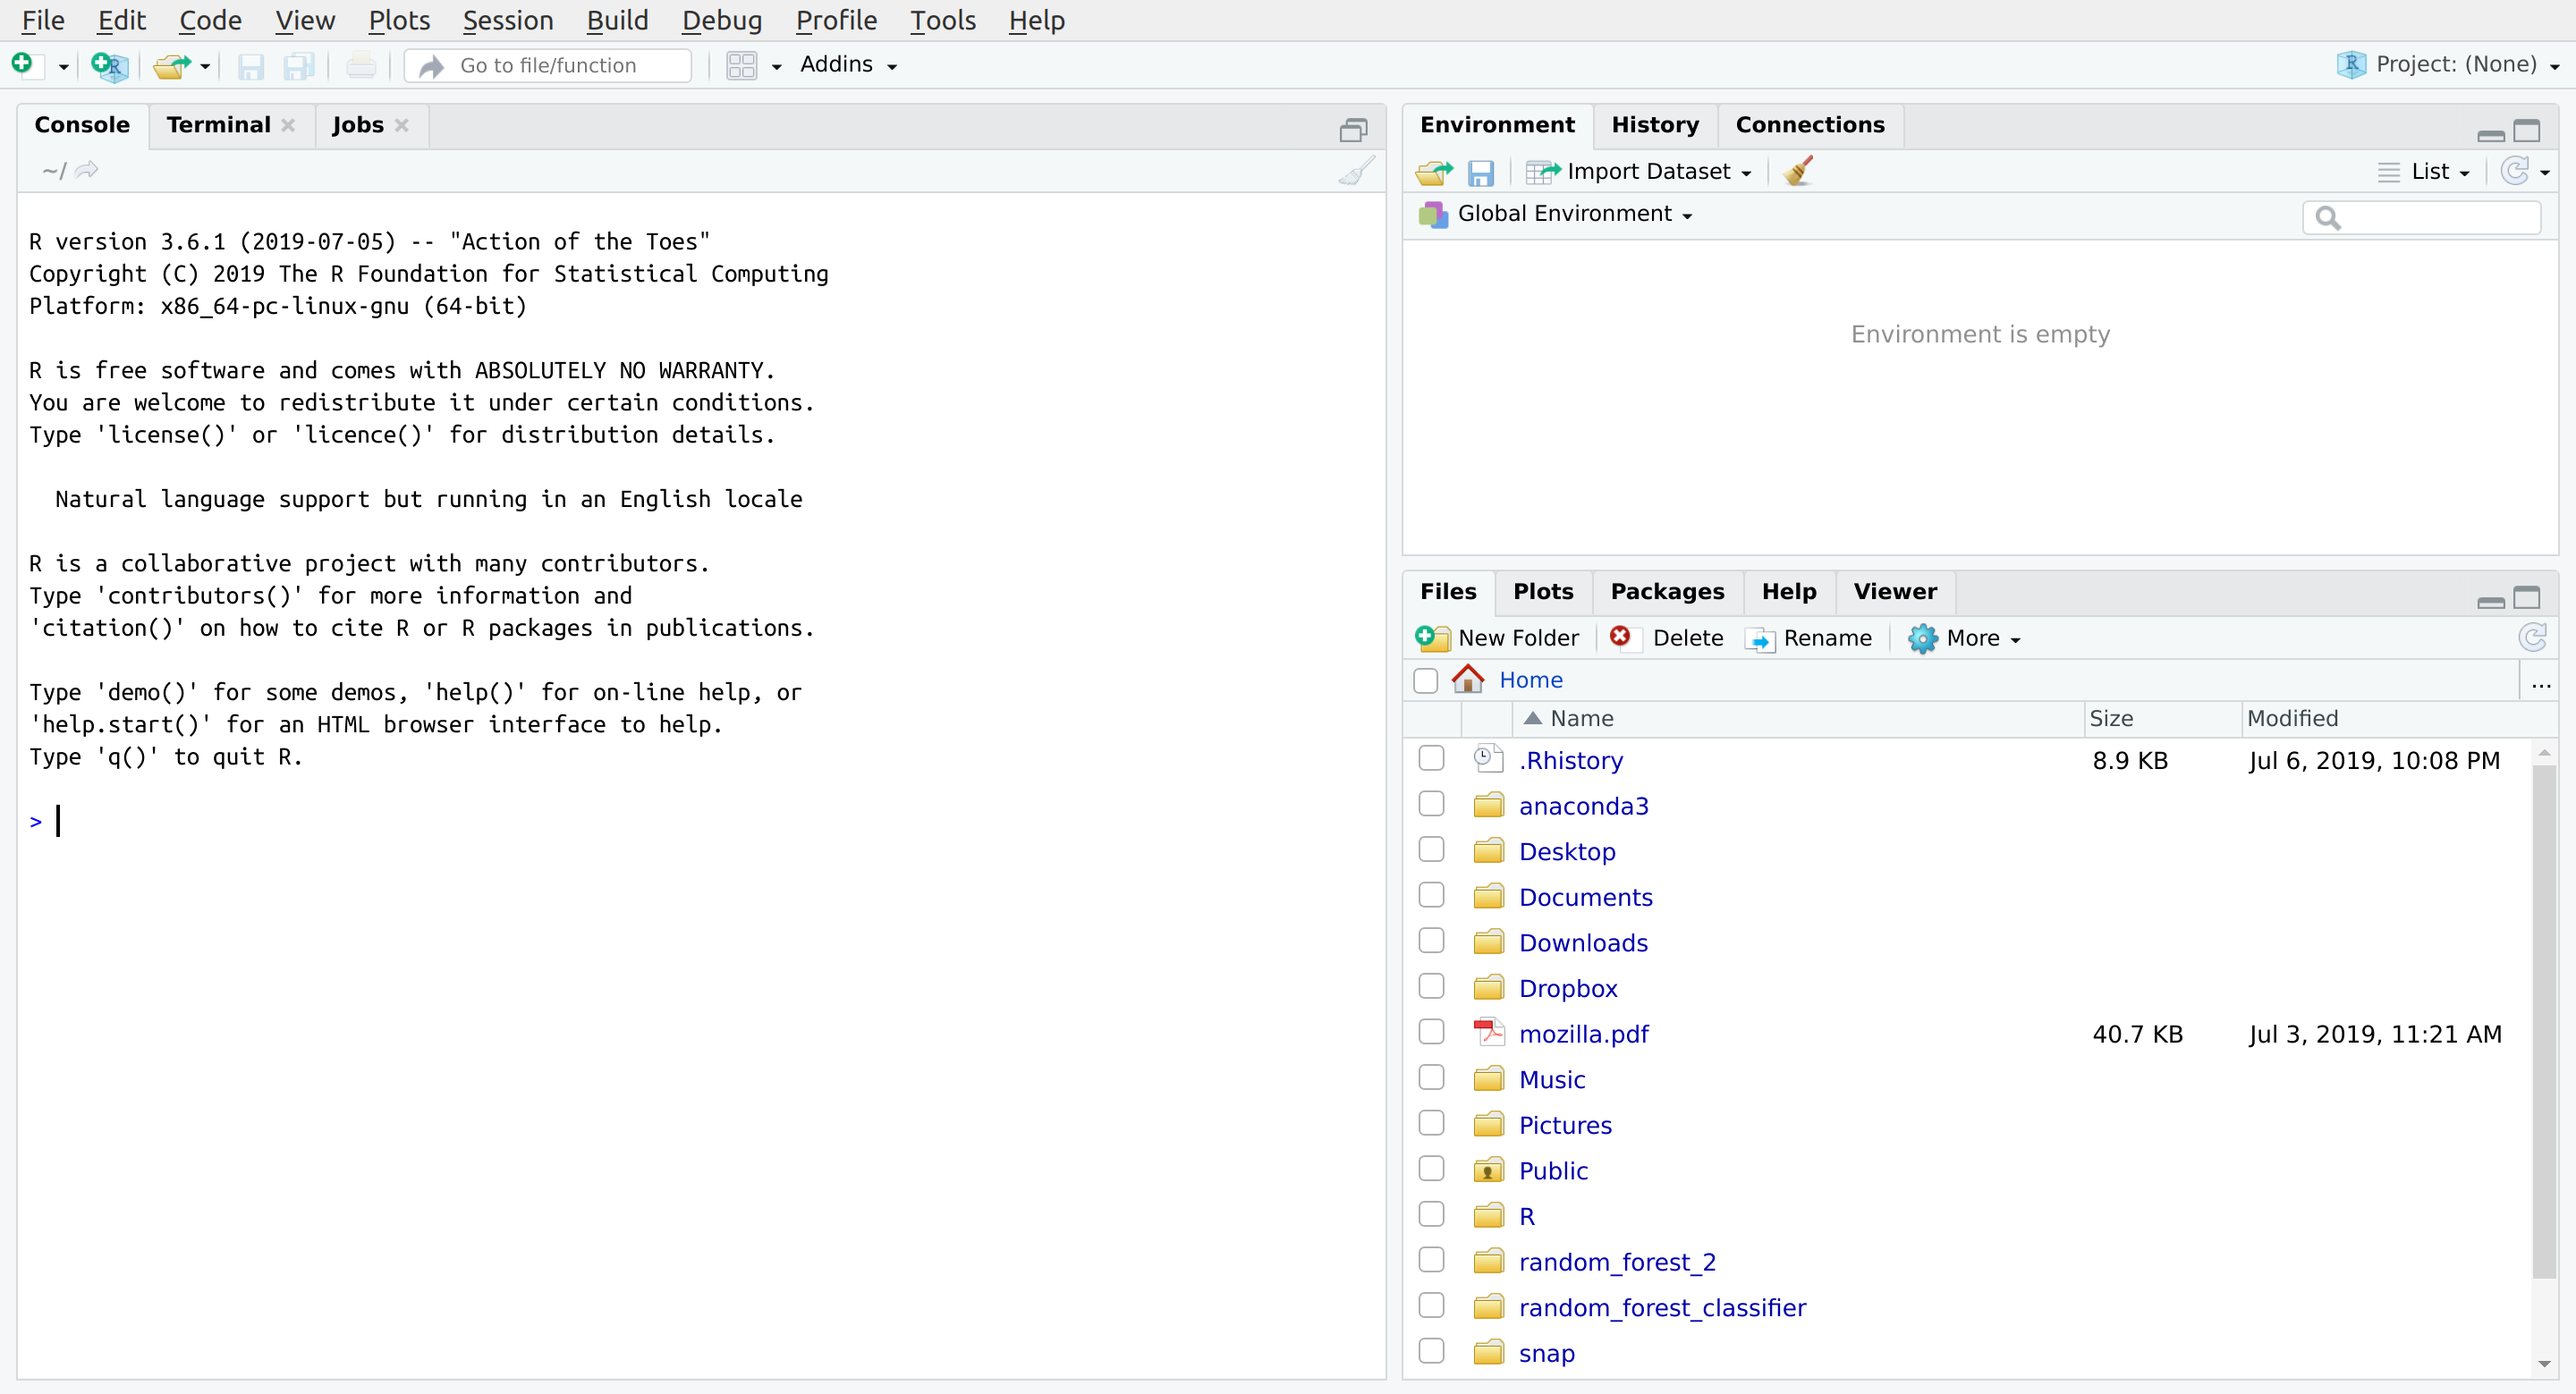
\includegraphics[width=40in]{images/RStudio1} 

}

\caption{La primera vez que abres RStudio}\label{fig:fig-main}
\end{figure}

Si tu RStudio tiene sólo 3 páneles, como en mi caso, ve a la esquina superior izquierda (signo de hoja+) y elige un nuevo \texttt{R\ Script}

\begin{figure}

{\centering 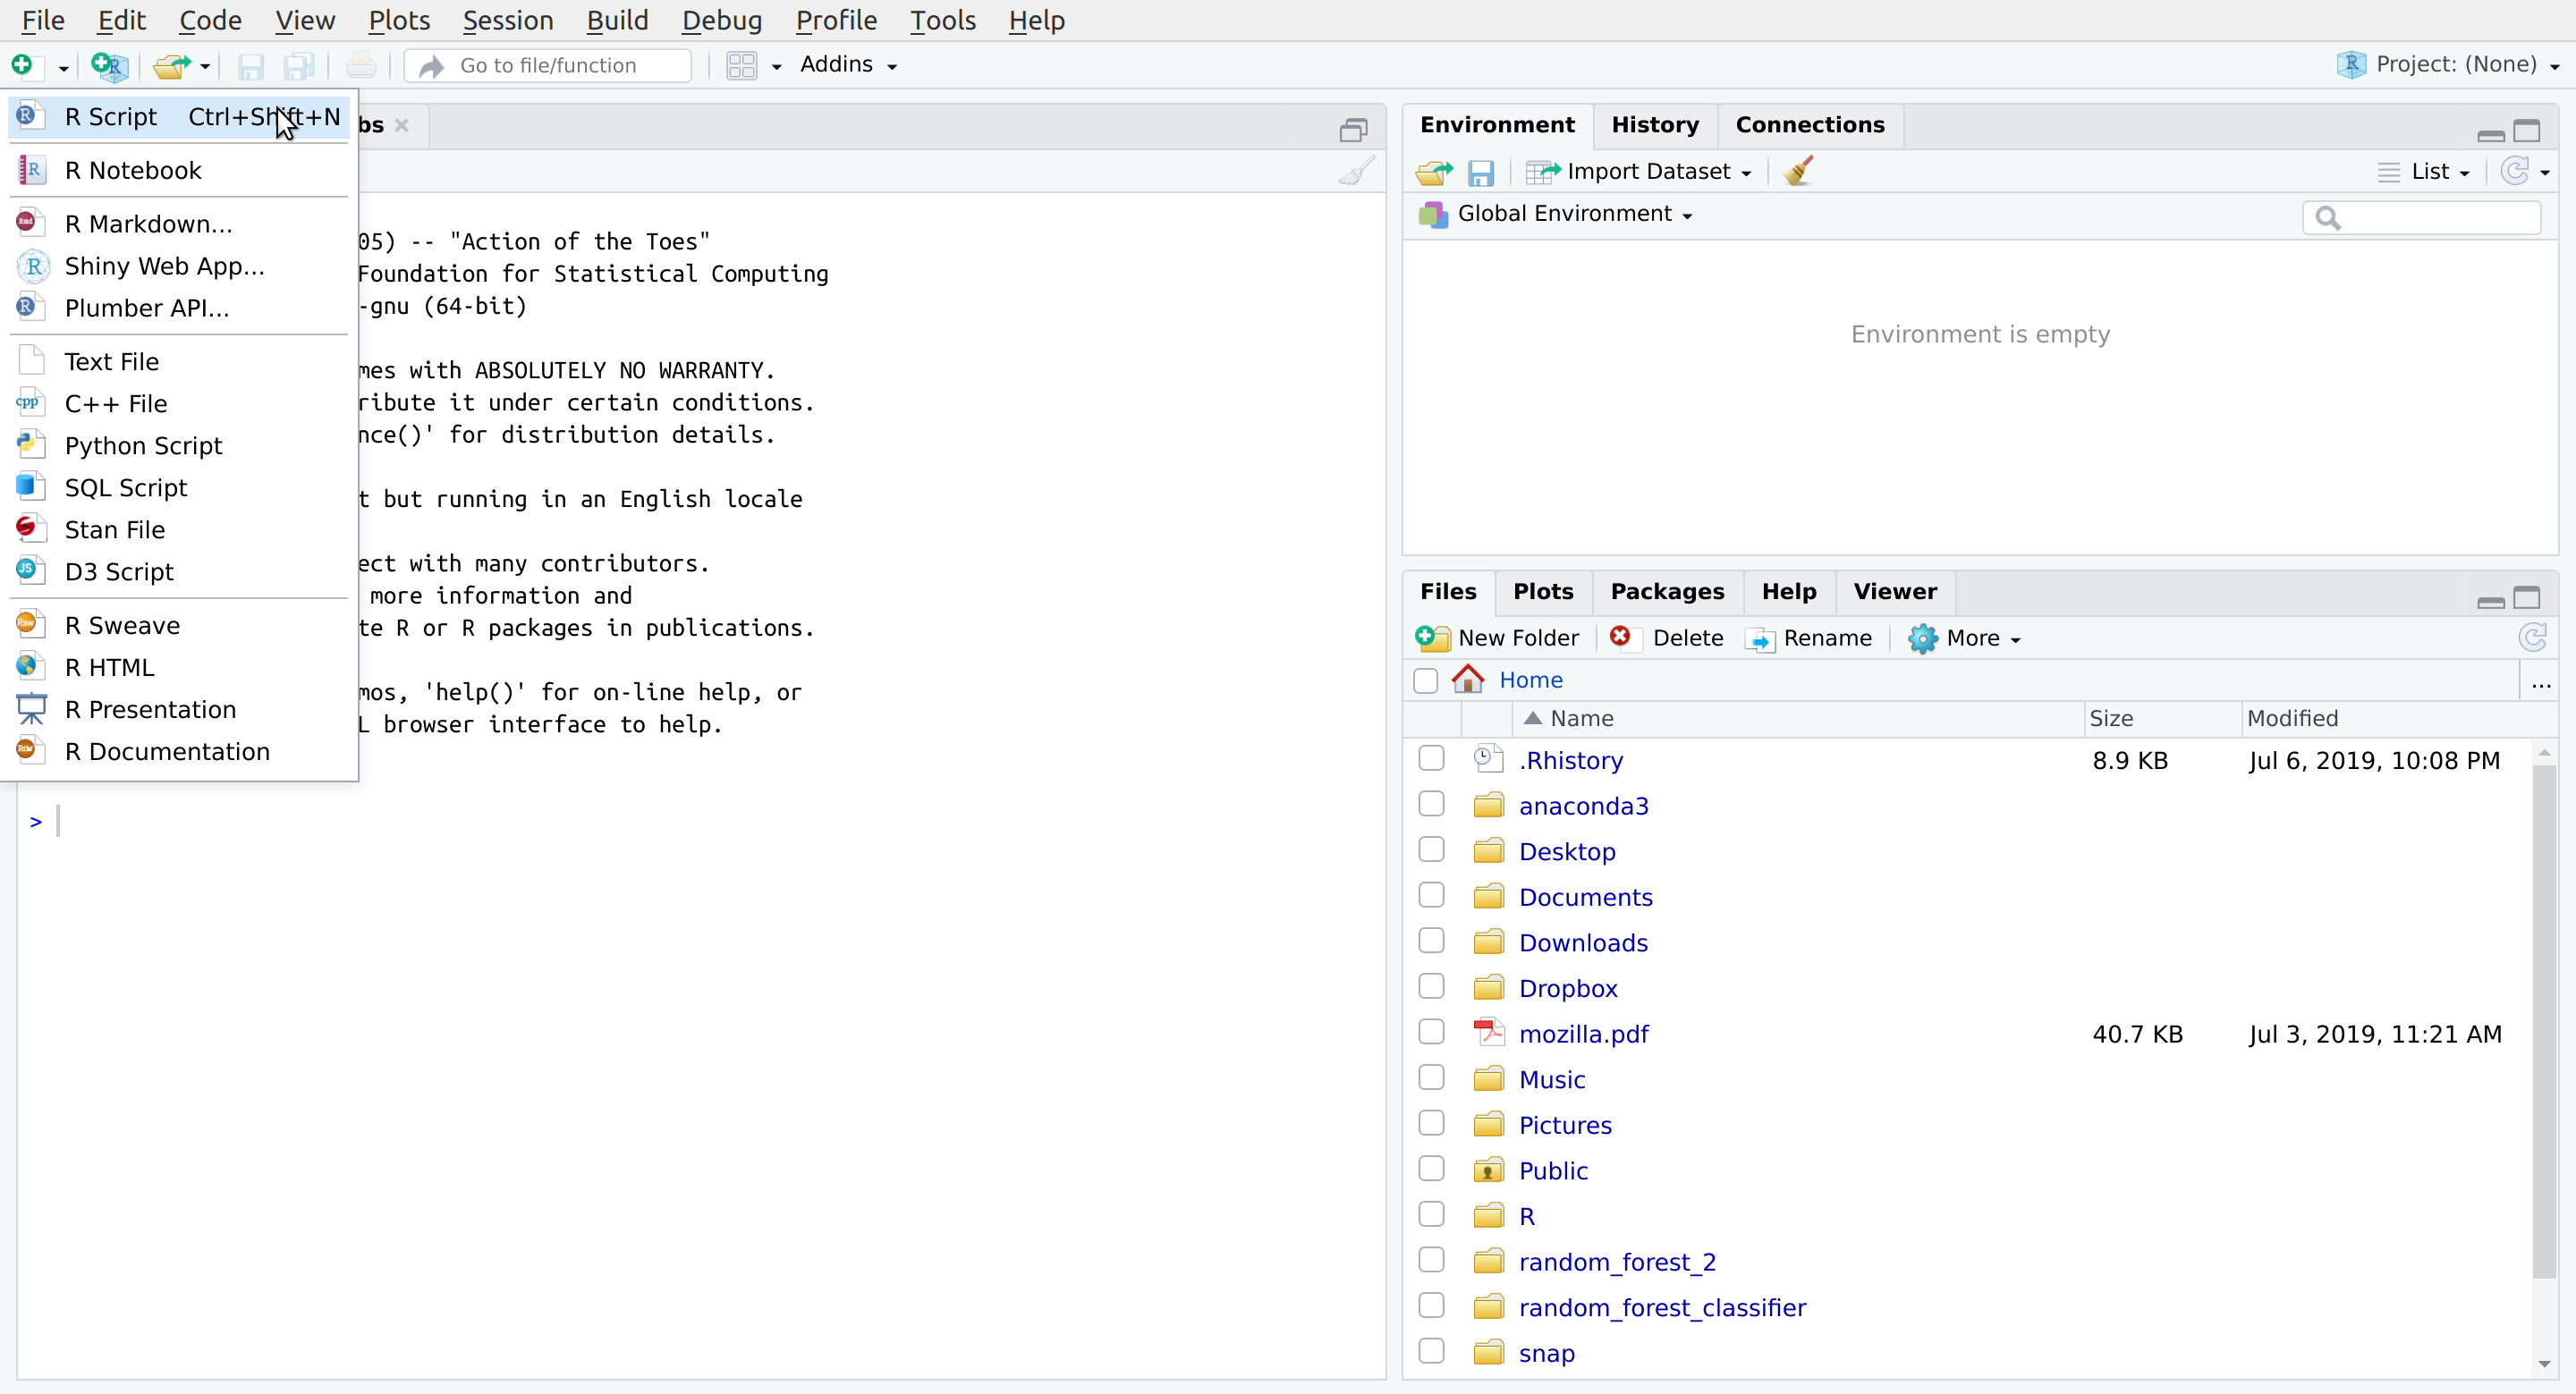
\includegraphics[width=40in]{images/RStudio2} 

}

\caption{Elige hoja+ para crear un nuevo archivo}\label{fig:unnamed-chunk-26}
\end{figure}

Tendrás, entonces, 4 páneles como se ve a continuación:

\begin{figure}

{\centering 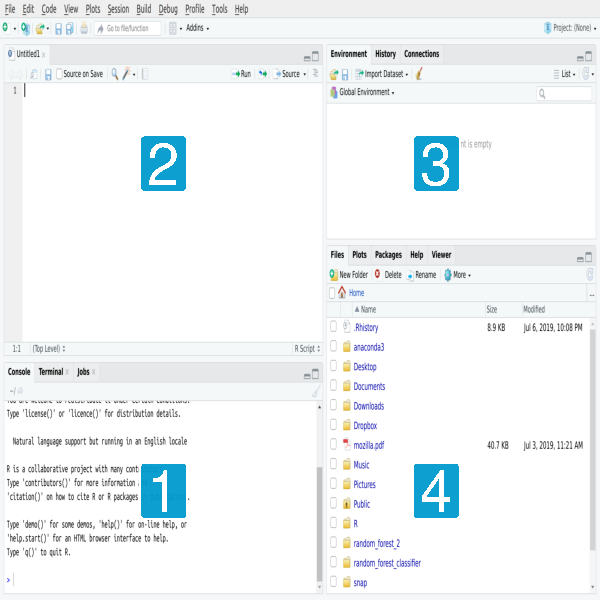
\includegraphics{InferenciaEstadistica_files/figure-latex/unnamed-chunk-27-1} 

}

\caption{RStudio <3}\label{fig:unnamed-chunk-27}
\end{figure}

\begin{enumerate}
\def\labelenumi{\arabic{enumi}.}
\tightlist
\item
  El primer panel (esquina inferior izquierda) es la \texttt{Consola}. Aquí es donde se ejecutan las acciones. Prueba escribir \texttt{2\ +\ 3} en él y presiona enter. Aparece el resultado de la suma. Definitivamente, \texttt{R} es la calculadora que más trabajo cuesta instalar.
\end{enumerate}

\begin{figure}

{\centering 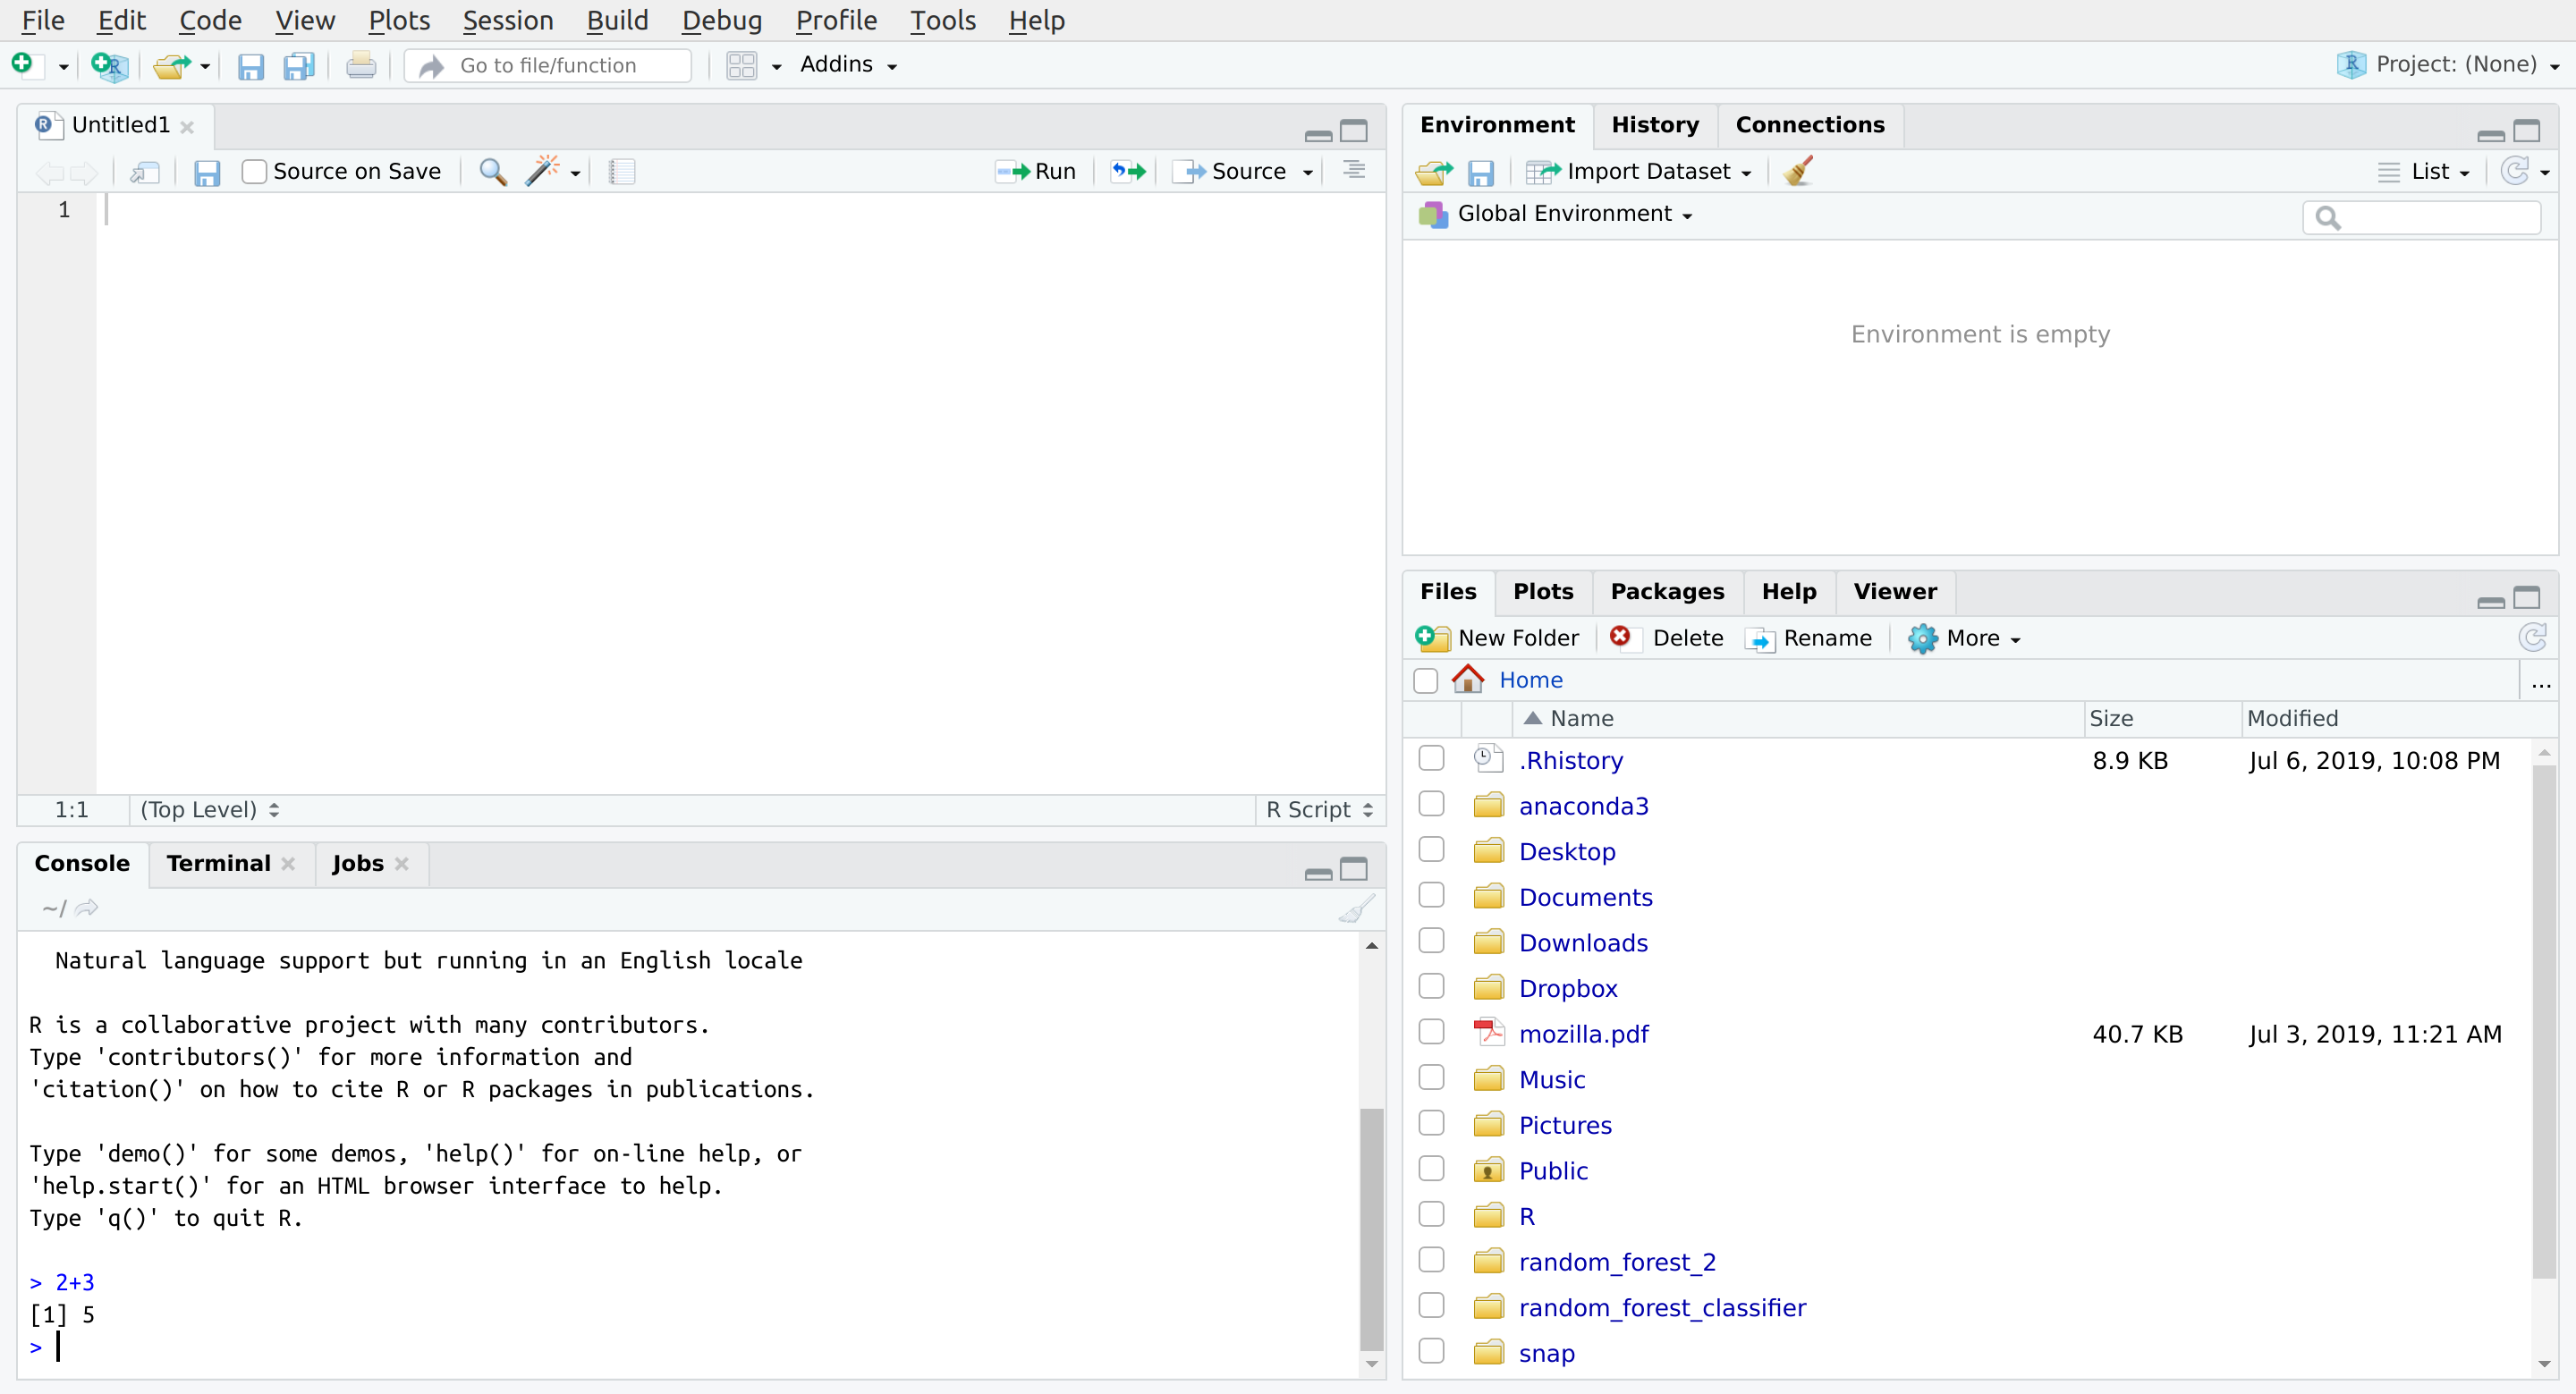
\includegraphics[width=40in]{images/RStudio4} 

}

\caption{La consola de `R` es la calculadora más difícil de instalar que existe.}\label{fig:unnamed-chunk-28}
\end{figure}

\begin{enumerate}
\def\labelenumi{\arabic{enumi}.}
\setcounter{enumi}{1}
\tightlist
\item
  El segundo panel (esquina superior izquierda) es el panel con el \texttt{Script}. Aquí se escribe el programa pero no \emph{se ejecuta}. Prueba escribir \texttt{10\ +\ 9}. ¿Ves que no pasa nada? Lo que acabas de hacer es crear un programa que, cuando se ejecute, hará la suma de \texttt{10\ +\ 9}. ¡Qué programa más aburrido! Sin embargo, no todo está perdido: presiona \texttt{CTRL+Enter} (\texttt{Cmd+Enter} en Mac) al final de la línea o bien da clic en \texttt{Run} y verás que, en la consola, aparece la instrucción y el resultado de la misma. El \texttt{Script} es una excelente fuente para tener un historial de lo que estás haciendo.
\end{enumerate}

\begin{figure}

{\centering 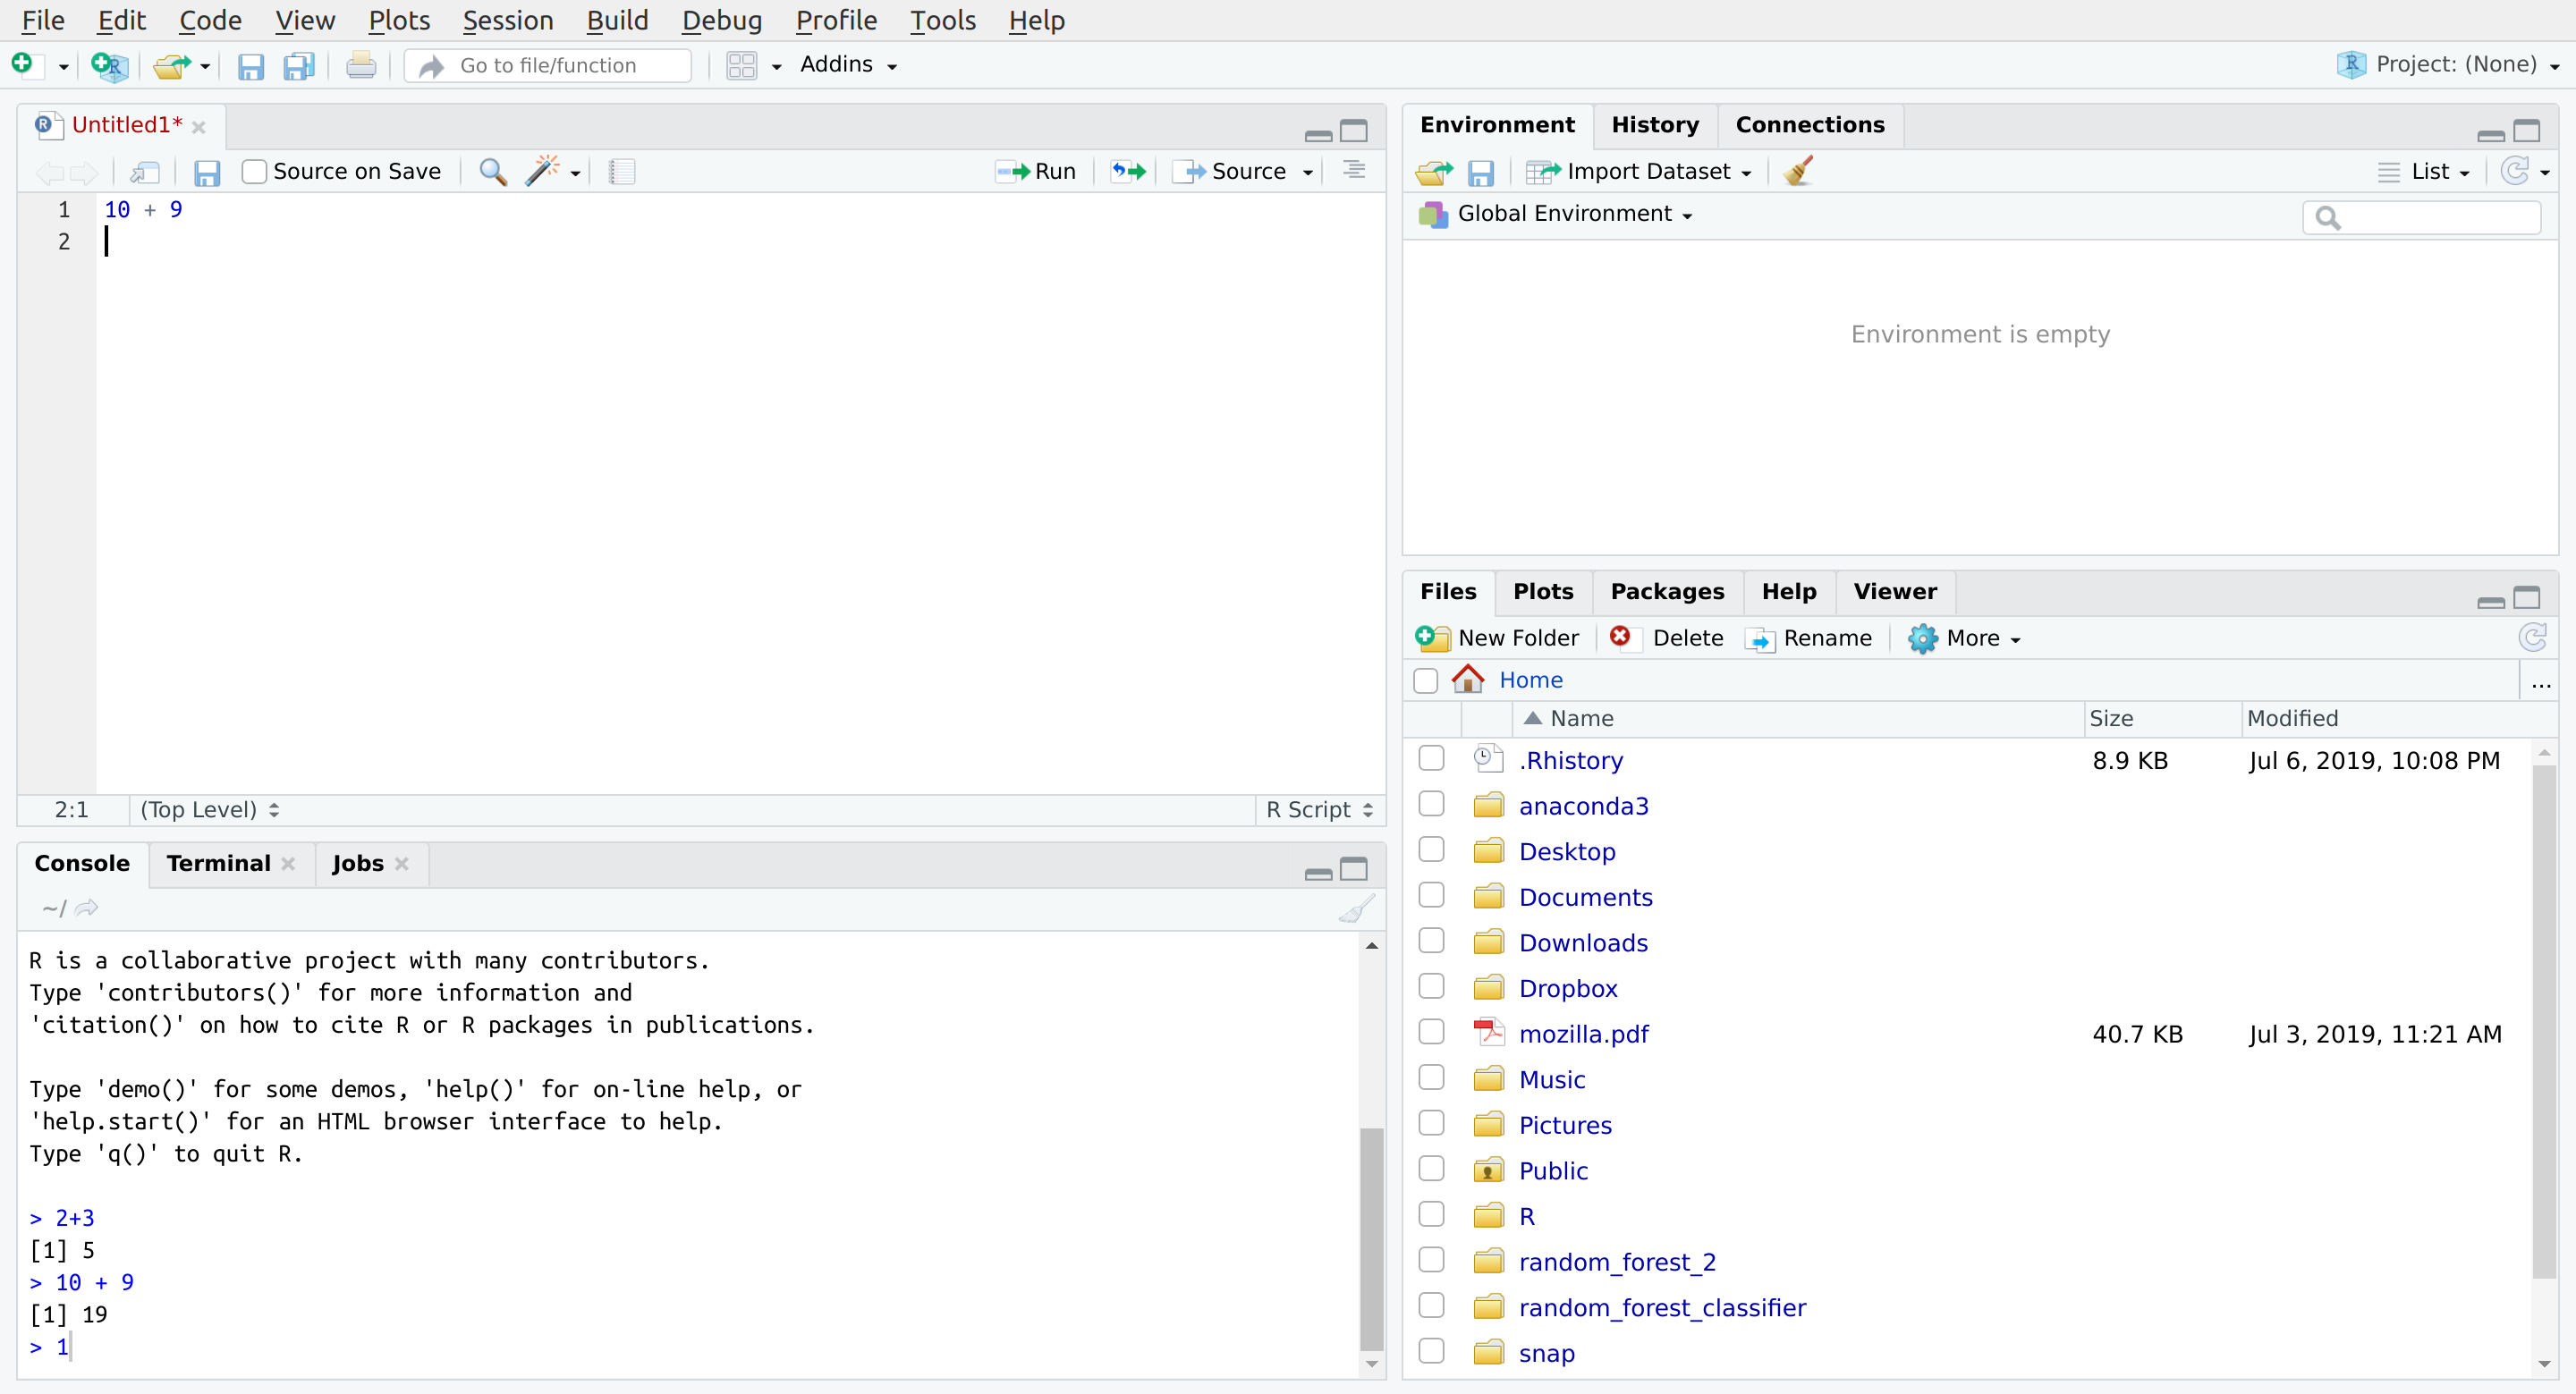
\includegraphics[width=40in]{images/RStudio5} 

}

\caption{El `Script` sirve para salvar las instrucciones en el orden en que las vas a ejecutar.}\label{fig:unnamed-chunk-29}
\end{figure}

\begin{enumerate}
\def\labelenumi{\arabic{enumi}.}
\setcounter{enumi}{2}
\tightlist
\item
  El tercer panel contiene el ambiente. Aquí aparecerán las variables que vayamos creando. Por ahora, para poner un ejemplo, importaremos el archivo \texttt{Example1.csv} (con valores simulados) \href{https://github.com/RodrigoZepeda/LibroEstadistica/tree/master/datasets}{disponible en Github} dando clic en \texttt{Import\ Dataset} y \texttt{From\ Text\ (base)}. Selecciona el archivo y elige las opciones en la ventana de previsualización que hagan que se vea bien. Nota que una vez realizada la importación aparece en el panel derecho \texttt{Example1.} Al dar clic podrás ver la base de datos. Las bases de datos y variables que utilices durante tus análisis aparecerán en esa sección.
\end{enumerate}

\begin{figure}

{\centering 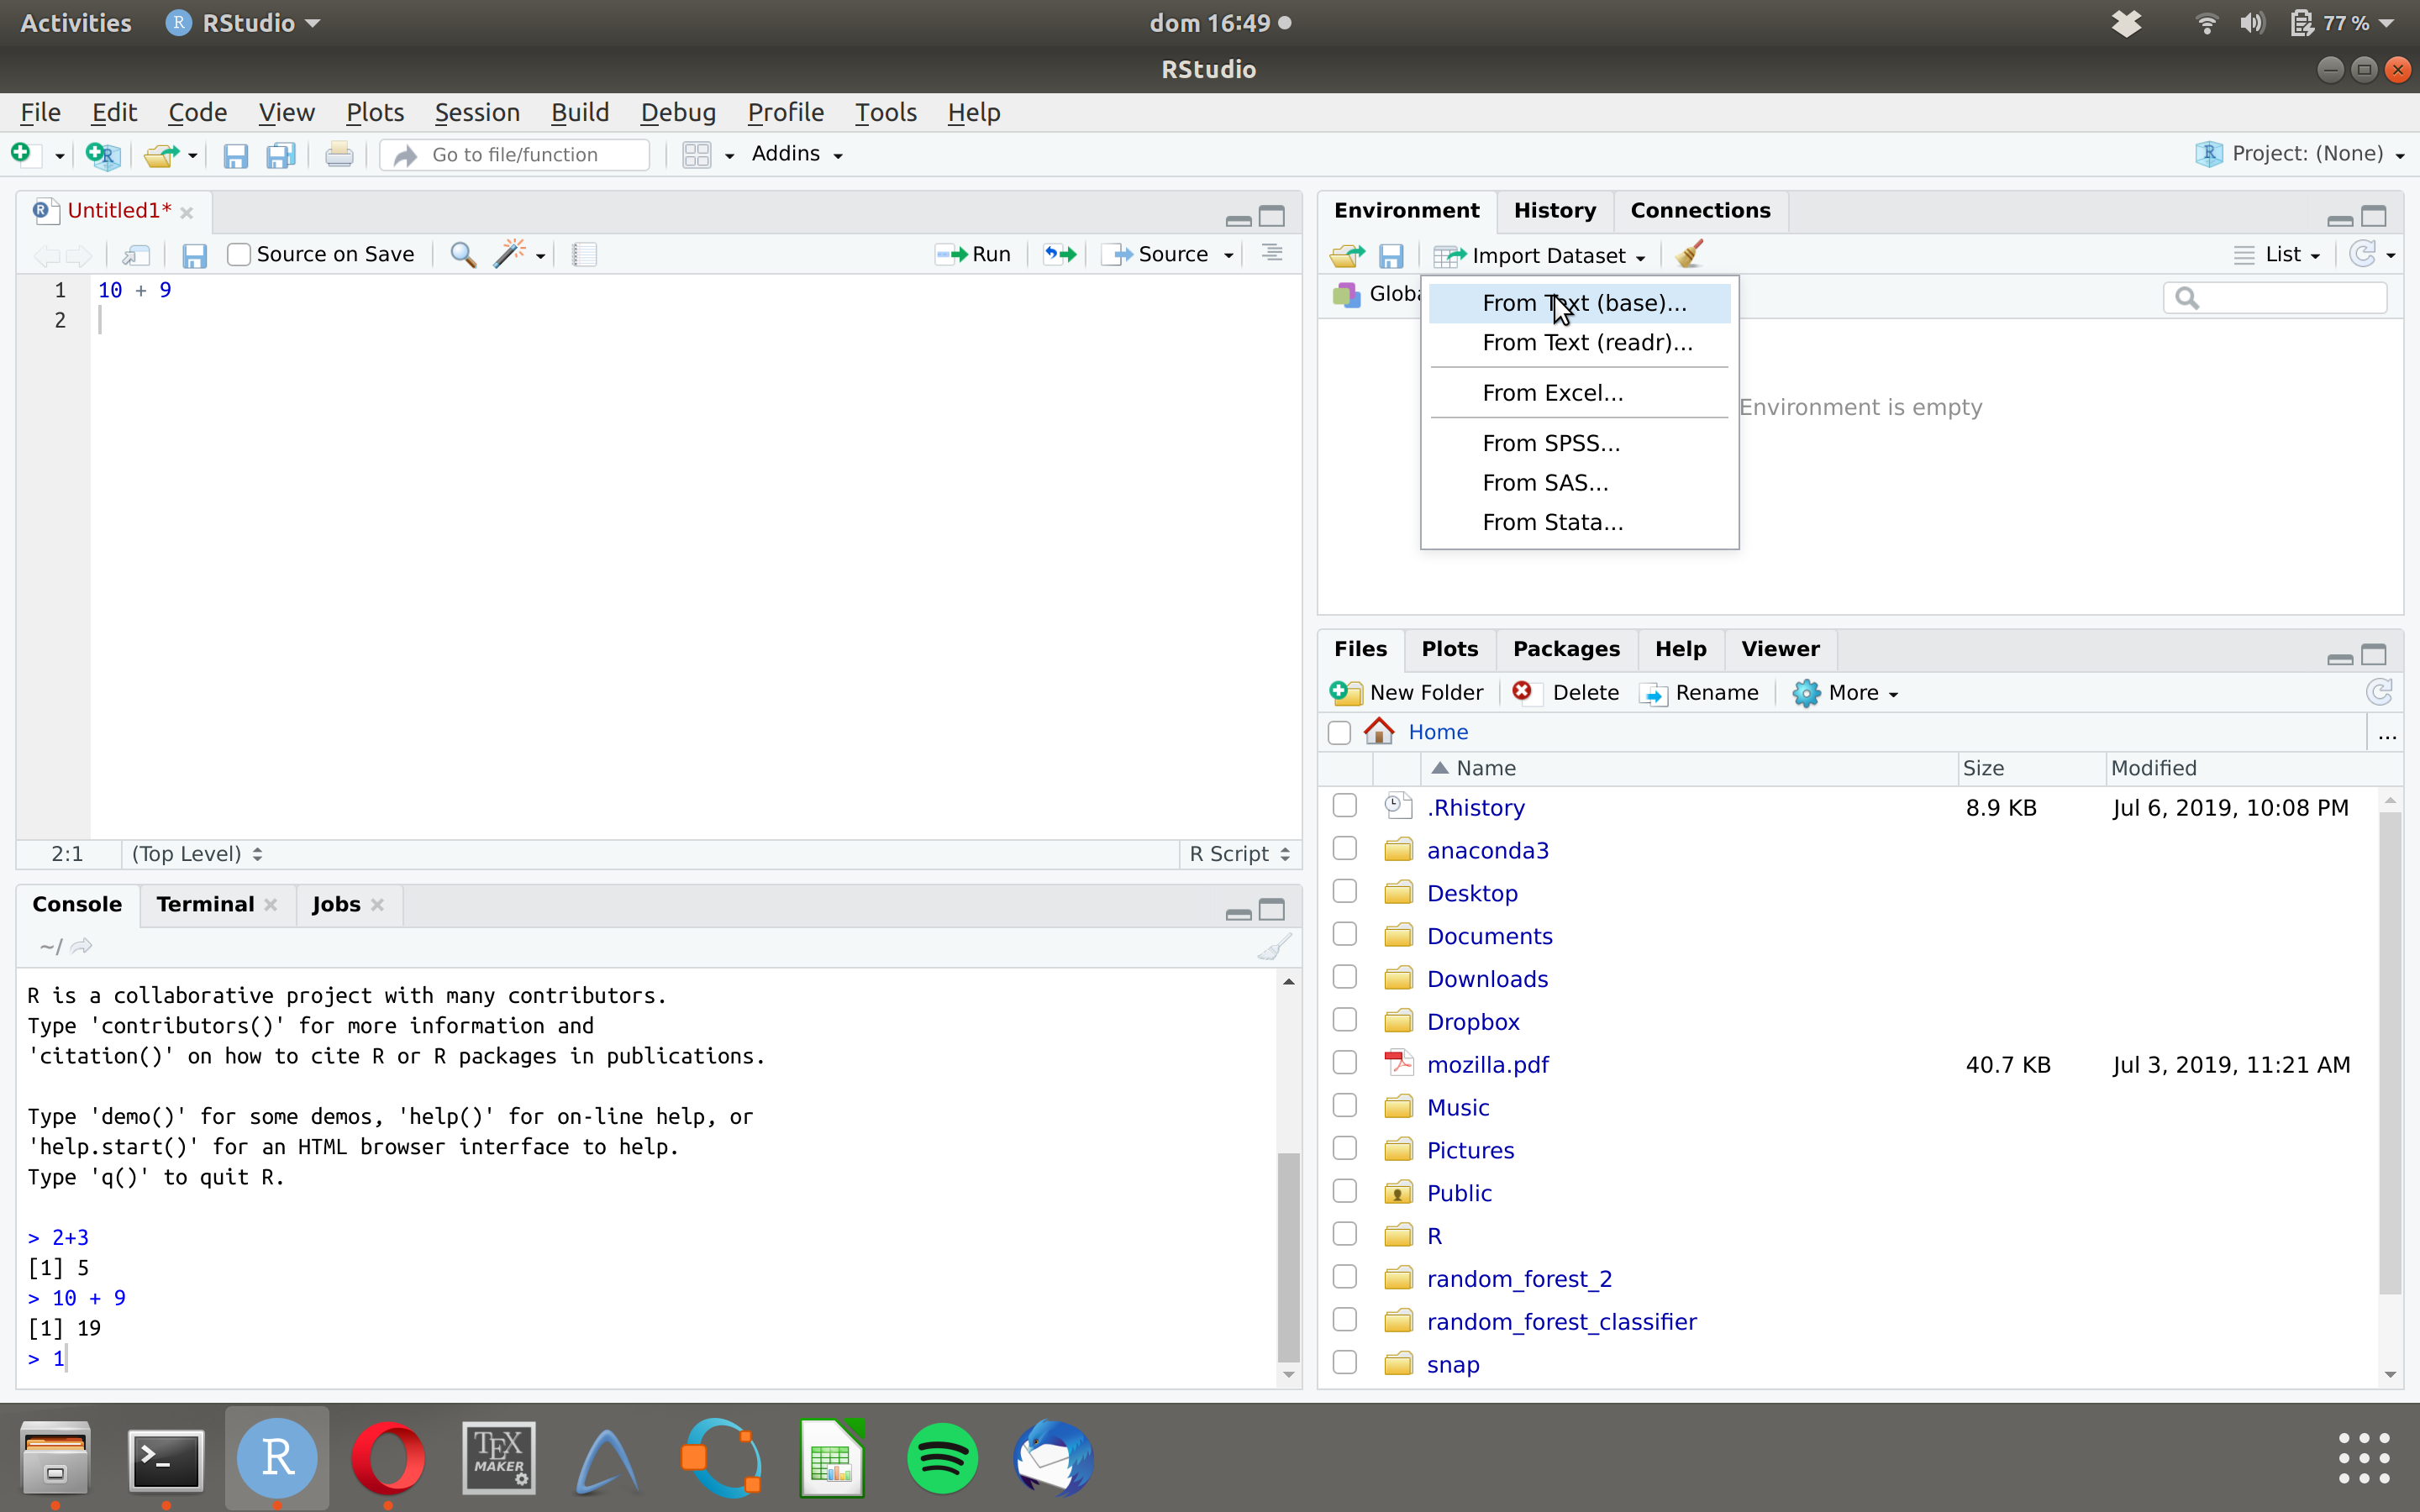
\includegraphics[width=40in]{images/RStudio6} 

}

\caption{El `Ambiente` muestra las variables (incluyendo bases de datos) que estás utilizando en este momento. A diferencia de otros programas estadísticos (o sea `Stata`) en `R` es posible tener múltiples bases de datos abiertas a la vez.}\label{fig:unnamed-chunk-31}
\end{figure}

\begin{enumerate}
\def\labelenumi{\arabic{enumi}.}
\setcounter{enumi}{3}
\tightlist
\item
  Para entender mejor lo que ocurre en el último de los páneles, lo mejor es trabajar con nuestra base. Escribe en la consola \texttt{plot(Example1)} . En el cuarto pánel aparecerá una gráfica. El cuarto de los páneles para nosotros tendrá esa utilidad: mostrará las gráficas que hagamos así como la ayuda. Para ver la ayuda para las instrucciones de \texttt{R} puedes escribir \texttt{?}. Prueba teclear \texttt{?plot} en la consola. El signo de interrogación es un \texttt{help()} que muestra las instrucciones para usar una función.
\end{enumerate}

\begin{figure}

{\centering 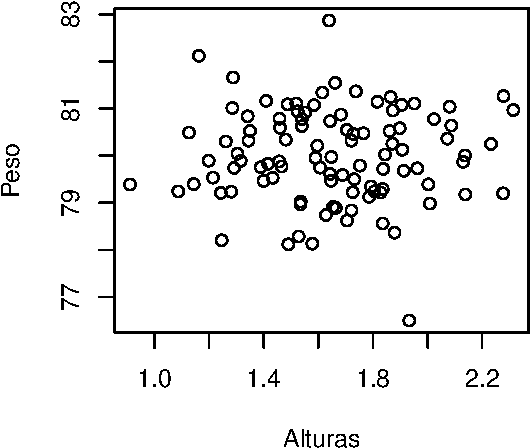
\includegraphics{InferenciaEstadistica_files/figure-latex/unnamed-chunk-32-1} 

}

\caption{La gráfica que aparece de hacer un `plot` de la base de datos de ejemplo.}\label{fig:unnamed-chunk-32}
\end{figure}

\begin{figure}

{\centering 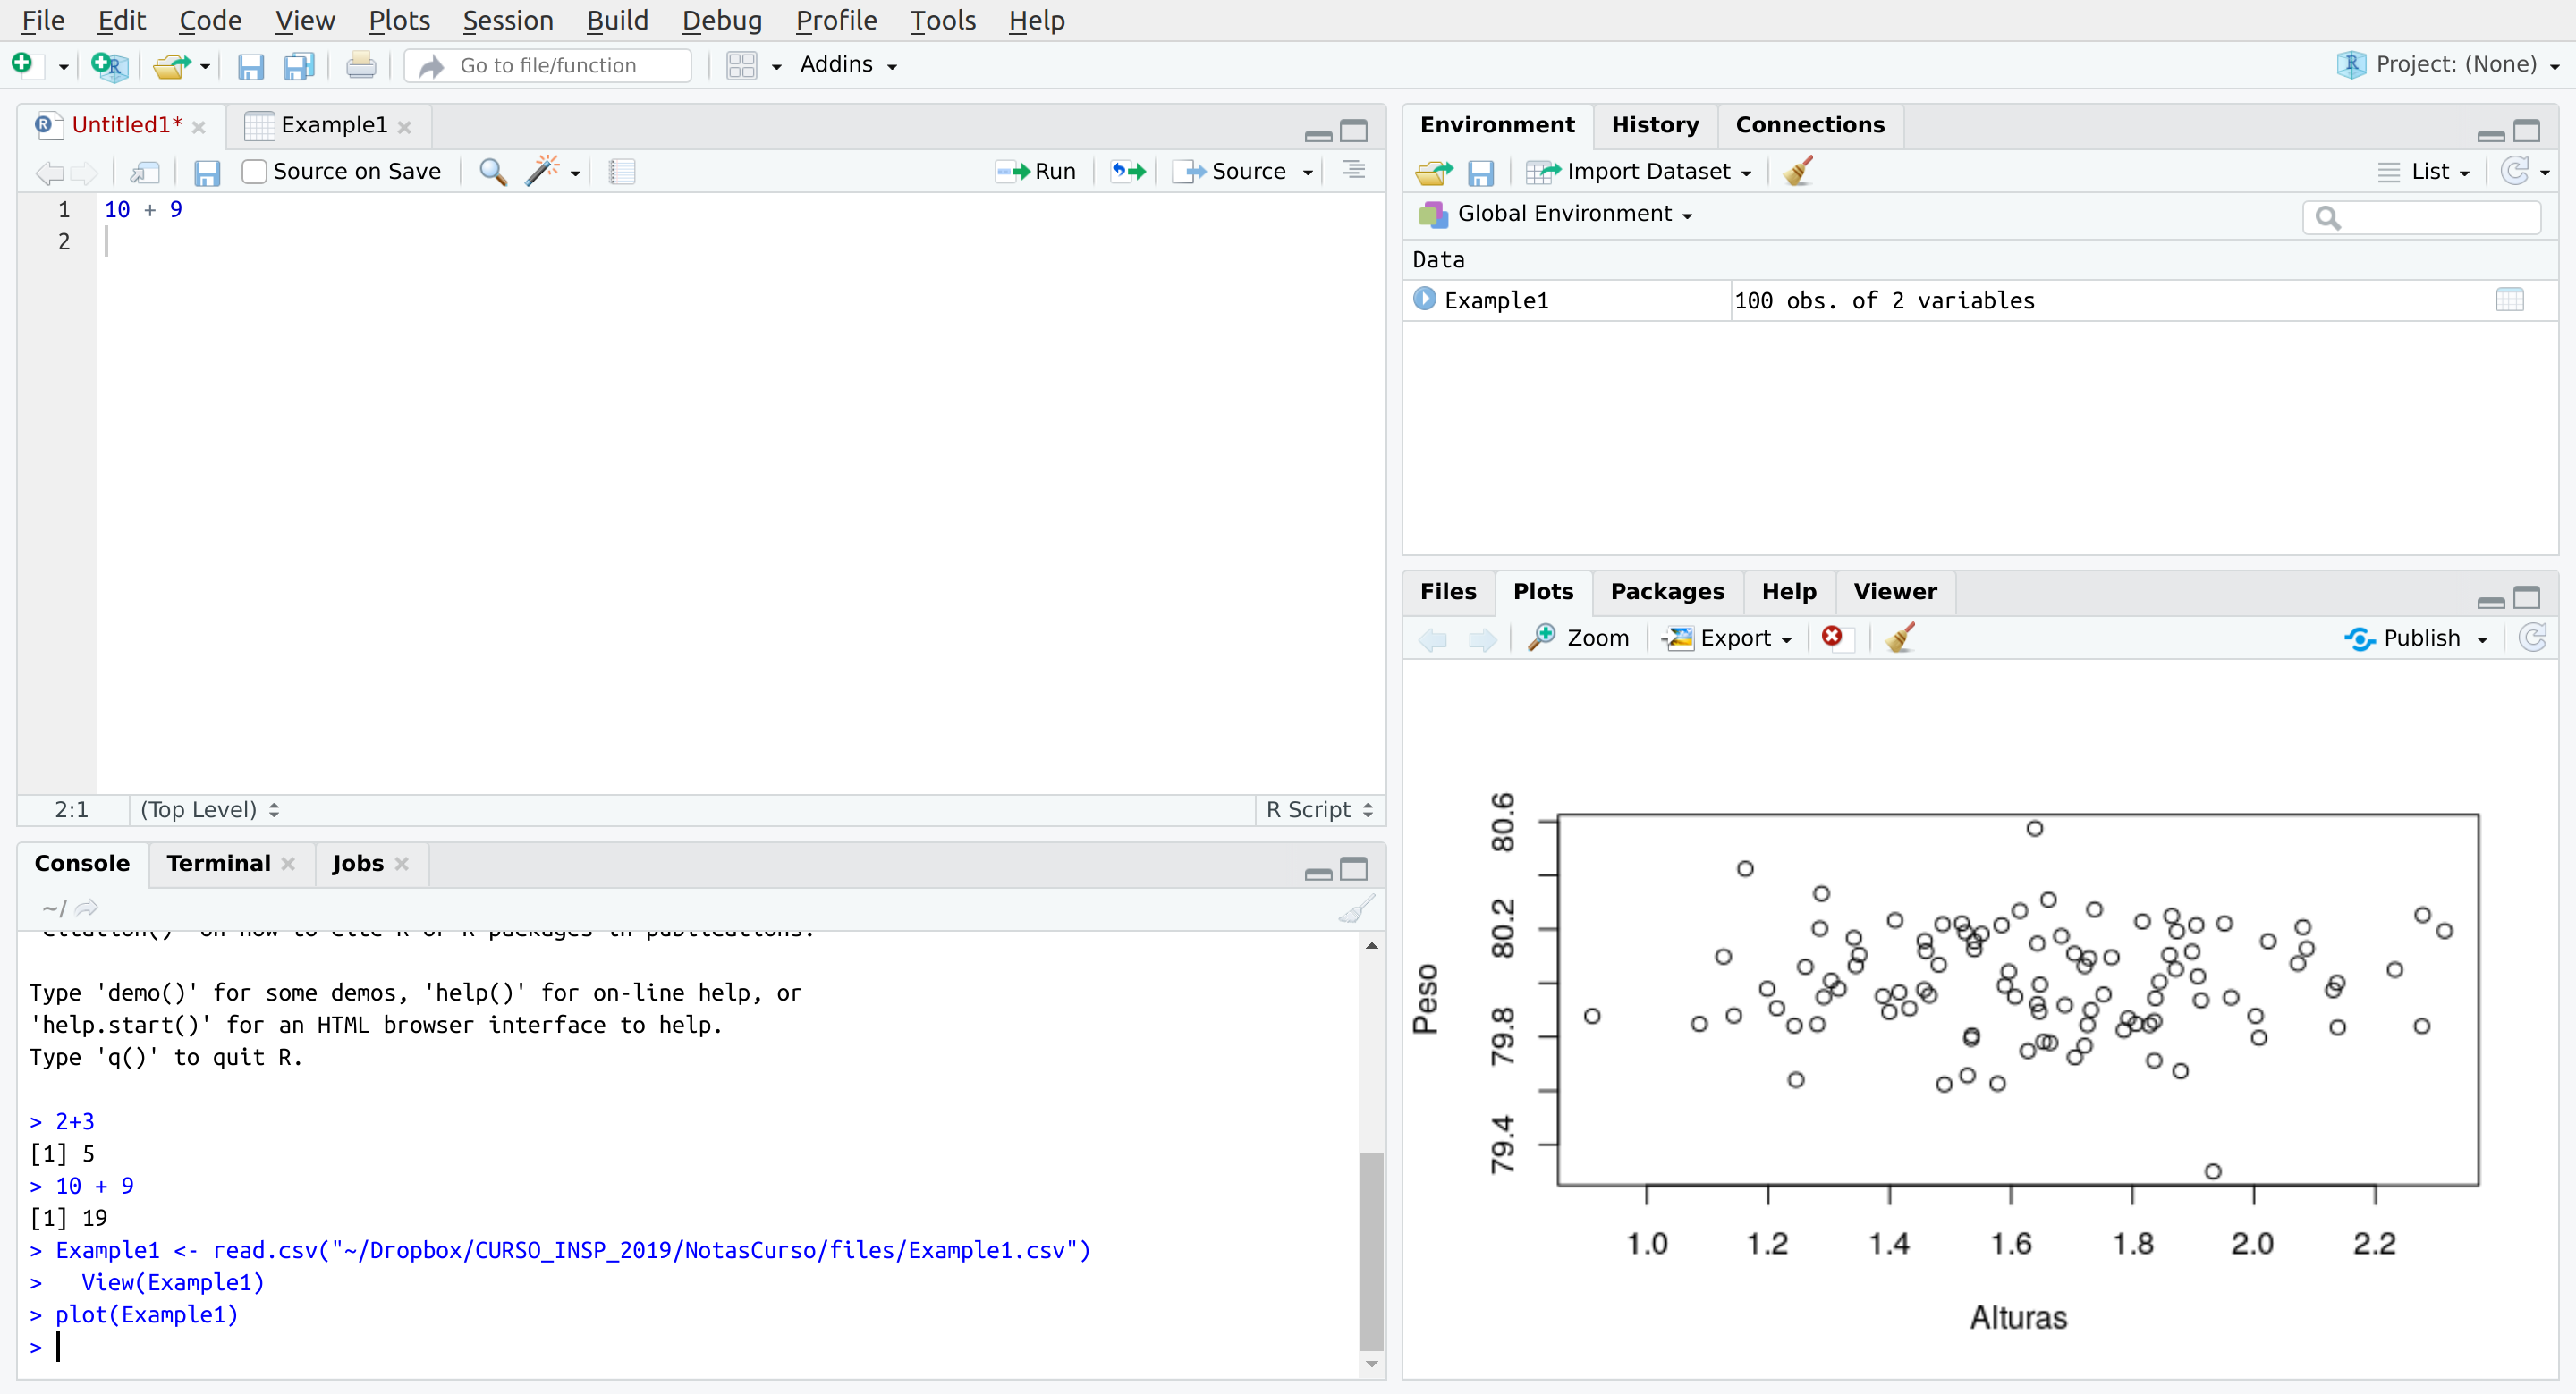
\includegraphics[width=40in]{images/RStudio7} 

}

\caption{El cuarto panel muestra respectivamente las gráficas y la ayuda.}\label{fig:unnamed-chunk-33}
\end{figure}

Mi sugerencia personal es que escribas todo lo que haces en el \texttt{Script} y que sólo utilices la consola para verificar valores. De esta manera podrás almacenar todas las instrucciones ejecutadas y volver a ellas cuando se requieran. Por último te sugiero utilizar \texttt{\#} gatos para comentar tu código. Así, el código anterior lo podrías ver en la consola como:

\begin{Shaded}
\begin{Highlighting}[]
\CommentTok{#Aquí pruebo cómo R hace las sumas}
\DecValTok{10} \OperatorTok{+}\StringTok{ }\DecValTok{9}
\end{Highlighting}
\end{Shaded}

\href{https://www.freecodecamp.org/news/code-comments-the-good-the-bad-and-the-ugly-be9cc65fbf83/}{Comenta}. \href{https://www.c-sharpcorner.com/blogs/why-comments-are-important-while-writing-a-code}{Comenta}. \href{https://blog.codinghorror.com/code-tells-you-how-comments-tell-you-why/}{Comenta, por favor}. Tu ser del futuro que regrese a sus archivos de \texttt{R} un mes después de haberlos hecho te lo agradecerá (y tu profe también).

Finalmente y como aclaración para estas notas, el código de \texttt{R} aparece como:

\begin{Shaded}
\begin{Highlighting}[]
\CommentTok{#Esto es código de R}
\DecValTok{7} \OperatorTok{-}\StringTok{ }\DecValTok{2}
\end{Highlighting}
\end{Shaded}

Mientras que los resultados de evaluar en \texttt{R} se ven con \texttt{\#}:
{[}1{]} 5

Así, la evaluación con su resultado se ve de la siguiente forma:

\begin{Shaded}
\begin{Highlighting}[]
\CommentTok{#Esto es código de R}
\DecValTok{7} \OperatorTok{-}\StringTok{ }\DecValTok{2}
\end{Highlighting}
\end{Shaded}

{[}1{]} 5

\hypertarget{cuxe1lculos-numuxe9ricos}{%
\section{Cálculos numéricos}\label{cuxe1lculos-numuxe9ricos}}

\texttt{R} sirve como calculadora para las operaciones usuales. En él puedes hacer sumas,

\begin{Shaded}
\begin{Highlighting}[]
\CommentTok{#Esto es una suma en R}
\DecValTok{12} \OperatorTok{+}\StringTok{ }\DecValTok{31}
\end{Highlighting}
\end{Shaded}

{[}1{]} 43

\begin{figure}

{\centering 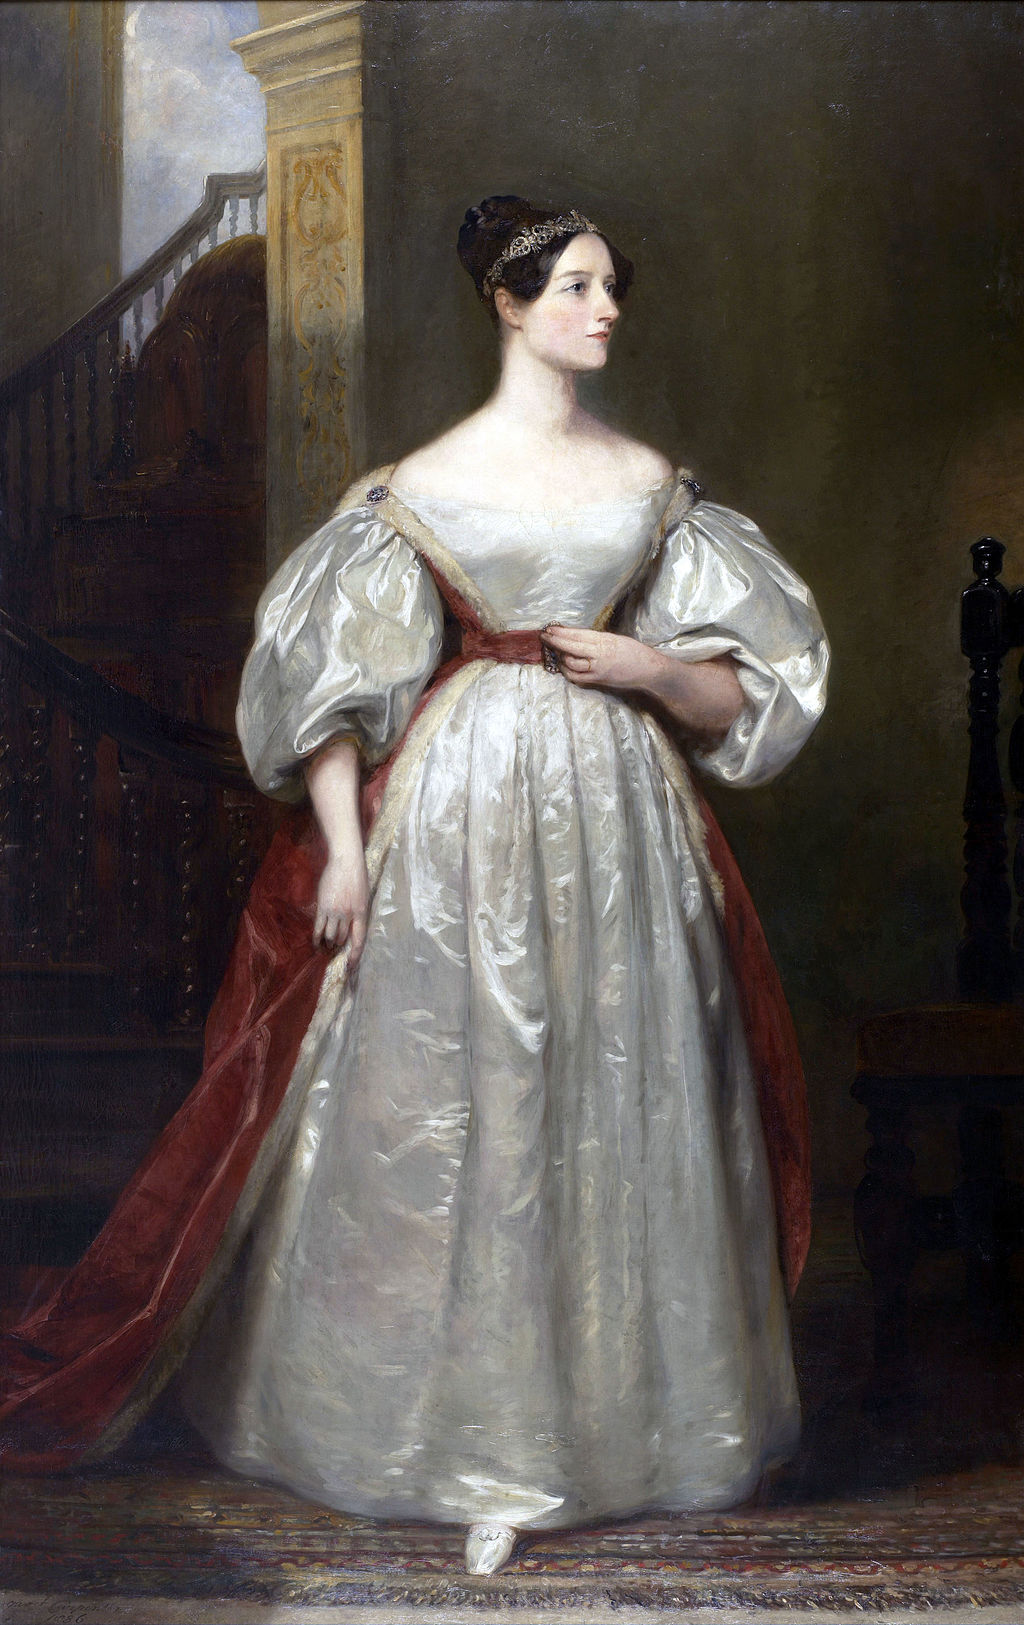
\includegraphics[width=14.22in]{images/ada_lovelace} 

}

\caption{Ada Lovelace (1815-1852), la primera en diseñar un algoritmo computacional ¡y sin tener computadoras!}\label{fig:unnamed-chunk-39}
\end{figure}

restas,

\begin{Shaded}
\begin{Highlighting}[]
\CommentTok{#Esto es una resta en R}
\DecValTok{3} \OperatorTok{-}\StringTok{ }\DecValTok{4}
\end{Highlighting}
\end{Shaded}

{[}1{]} -1

multiplicaciones,

\begin{Shaded}
\begin{Highlighting}[]
\CommentTok{#Esto es una multiplicación en R}
\DecValTok{7}\OperatorTok{*}\DecValTok{8}
\end{Highlighting}
\end{Shaded}

{[}1{]} 56

divisiones,

\begin{Shaded}
\begin{Highlighting}[]
\CommentTok{#Esto es una división en R}
\DecValTok{4}\OperatorTok{/}\DecValTok{2}
\end{Highlighting}
\end{Shaded}

{[}1{]} 2

sacar logaritmos naturales \(\ln\),

\begin{Shaded}
\begin{Highlighting}[]
\CommentTok{#Para sacar logaritmo usas el comando log}
\KeywordTok{log}\NormalTok{(}\DecValTok{100}\NormalTok{)}
\end{Highlighting}
\end{Shaded}

{[}1{]} 4.60517

o bien logaritmos en cualquier base,\footnote{Recuerda que un logaritmo base \(a\) te dice a qué potencia \(b\) tuve que elevar \(a\) para llegar a \(b\). Por ejemplo \(\log_{10}(100) = 2\) te dice que para llegar al \(100\) tuviste que hacer \(10^2\).}

\begin{Shaded}
\begin{Highlighting}[]
\CommentTok{#Puedes especificar la base del logaritmo con base }
\KeywordTok{log}\NormalTok{(}\DecValTok{100}\NormalTok{, }\DataTypeTok{base =} \DecValTok{10}\NormalTok{)}
\end{Highlighting}
\end{Shaded}

{[}1{]} 2

también puedes elevar a una potencia (por ejemplo hacer \(6^3\)),

\begin{Shaded}
\begin{Highlighting}[]
\CommentTok{#Así se calculan potencias}
\DecValTok{6}\OperatorTok{^}\DecValTok{3}
\end{Highlighting}
\end{Shaded}

{[}1{]} 216

calcular la exponencial \(e\),

\begin{Shaded}
\begin{Highlighting}[]
\CommentTok{#Para exponenciales puedes usar exp}
\KeywordTok{exp}\NormalTok{(}\DecValTok{1}\NormalTok{)}
\end{Highlighting}
\end{Shaded}

{[}1{]} 2.718282

o bien exponenciar cualquier variable \(e^{-3}\),

\begin{Shaded}
\begin{Highlighting}[]
\CommentTok{#O bien exponenciales específicas, e^-3}
\KeywordTok{exp}\NormalTok{(}\OperatorTok{-}\DecValTok{3}\NormalTok{)}
\end{Highlighting}
\end{Shaded}

{[}1{]} 0.04978707

también puedes usar el número \(\pi\).

\begin{Shaded}
\begin{Highlighting}[]
\CommentTok{#Cálculo de pi}
\NormalTok{pi}
\end{Highlighting}
\end{Shaded}

{[}1{]} 3.141593

No olvides que \texttt{R} usa el orden de las operaciones de matemáticas. Siempre es de izquierda a derecha con las siguientes excepciones:

\begin{enumerate}
\def\labelenumi{\arabic{enumi}.}
\item
  Primero se evalúa lo que está entre paréntesis.
\item
  En segundo lugar se calculan potencias.
\item
  Lo tercero en evaluarse son multiplicaciones y divisiones.
\item
  Finalmente, se realizan sumas y restas.
\end{enumerate}

Por ejemplo, en la siguiente ecuación
\[
2 - 2 \cdot \frac{(3^4 - 9)}{(5 + 4)}
\]
se resuelven primero los paréntesis \((3^4 - 9) = 81 - 9 = 72\) y \((5 + 4) = 9\); luego se resuelve la división: \(\frac{72}{9}=8\), se multiplica por el \(2\): \(2 \cdot 8 = 16\) y finalmente se hace la resta: \(2-16 = -14\).

\hypertarget{ejercicio}{%
\subsection{Ejercicio}\label{ejercicio}}

Determina, sin evaluar, los resultados de los siguientes segmentos de código:

\begin{Shaded}
\begin{Highlighting}[]
\CommentTok{#Primer ejercicio }
\NormalTok{(}\DecValTok{9} \OperatorTok{-}\StringTok{ }\DecValTok{3}\NormalTok{)}\OperatorTok{^}\DecValTok{2} \OperatorTok{*}\StringTok{ }\NormalTok{(}\DecValTok{2} \OperatorTok{-}\StringTok{ }\DecValTok{1}\NormalTok{) }\OperatorTok{-}\StringTok{ }\DecValTok{6}
\end{Highlighting}
\end{Shaded}

\begin{Shaded}
\begin{Highlighting}[]
\CommentTok{#Segundo ejercicio }
\DecValTok{6} \OperatorTok{*}\StringTok{ }\DecValTok{2} \OperatorTok{/}\StringTok{ }\NormalTok{(}\DecValTok{7} \OperatorTok{-}\StringTok{ }\DecValTok{3}\NormalTok{) }\OperatorTok{*}\StringTok{ }\DecValTok{5}
\end{Highlighting}
\end{Shaded}

\begin{Shaded}
\begin{Highlighting}[]
\CommentTok{#Tercer ejercicio }
\DecValTok{2} \OperatorTok{*}\StringTok{ }\DecValTok{3} \OperatorTok{^}\StringTok{ }\DecValTok{2} \OperatorTok{*}\StringTok{ }\DecValTok{2} \OperatorTok{/}\StringTok{ }\NormalTok{(}\DecValTok{5} \OperatorTok{-}\StringTok{ }\DecValTok{4}\NormalTok{) }\OperatorTok{*}\StringTok{ }\DecValTok{1} \OperatorTok{/}\StringTok{ }\DecValTok{10} 
\end{Highlighting}
\end{Shaded}

Evalúa para comprobar tu respuesta.

\hypertarget{ejercicio-1}{%
\subsection{Ejercicio}\label{ejercicio-1}}

Calcula el área y el perímetro de un círculo de radio 5. Recuerda que la fórmula del área es \(\pi \cdot r^2\) donde \(r\) es el radio; mientras que la del perímetro es: \(\pi \cdot d\) donde \(d\) es el díametro (= dos veces el radio).

\hypertarget{respuestas}{%
\subsection{Respuestas}\label{respuestas}}

Área = 78.5398163397448
Perímetro = 31.4159265358979

\hypertarget{variables}{%
\section{Variables}\label{variables}}

\texttt{R} es un programa orientado a objetos; esto quiere decir que \texttt{R} almacena la información en un conjunto de variables que pueden tener diferentes \texttt{clases} y opera con ellos según su clase. Por ejemplo, un conjunto de caracteres, entre comillas, es un \texttt{Character} (\texttt{R} lo piensa como texto)

\begin{Shaded}
\begin{Highlighting}[]
\CommentTok{#Un conjunto de caracteres es un char}
\StringTok{"Hola"}
\end{Highlighting}
\end{Shaded}

{[}1{]} ``Hola''

Un número (por ejemplo \texttt{2} tiene clase \texttt{numeric})\footnote{Puede ser \texttt{float}, \texttt{int}, \texttt{double} pero no nos preocuparemos por eso.}. Hay que tener mucho cuidado con combinar floats con \texttt{Strings}:

\begin{Shaded}
\begin{Highlighting}[]
\CommentTok{#Código que sí funciona porque ambos son números}
\DecValTok{2} \OperatorTok{+}\StringTok{ }\DecValTok{4} 
\end{Highlighting}
\end{Shaded}

{[}1{]} 6

\begin{figure}

{\centering 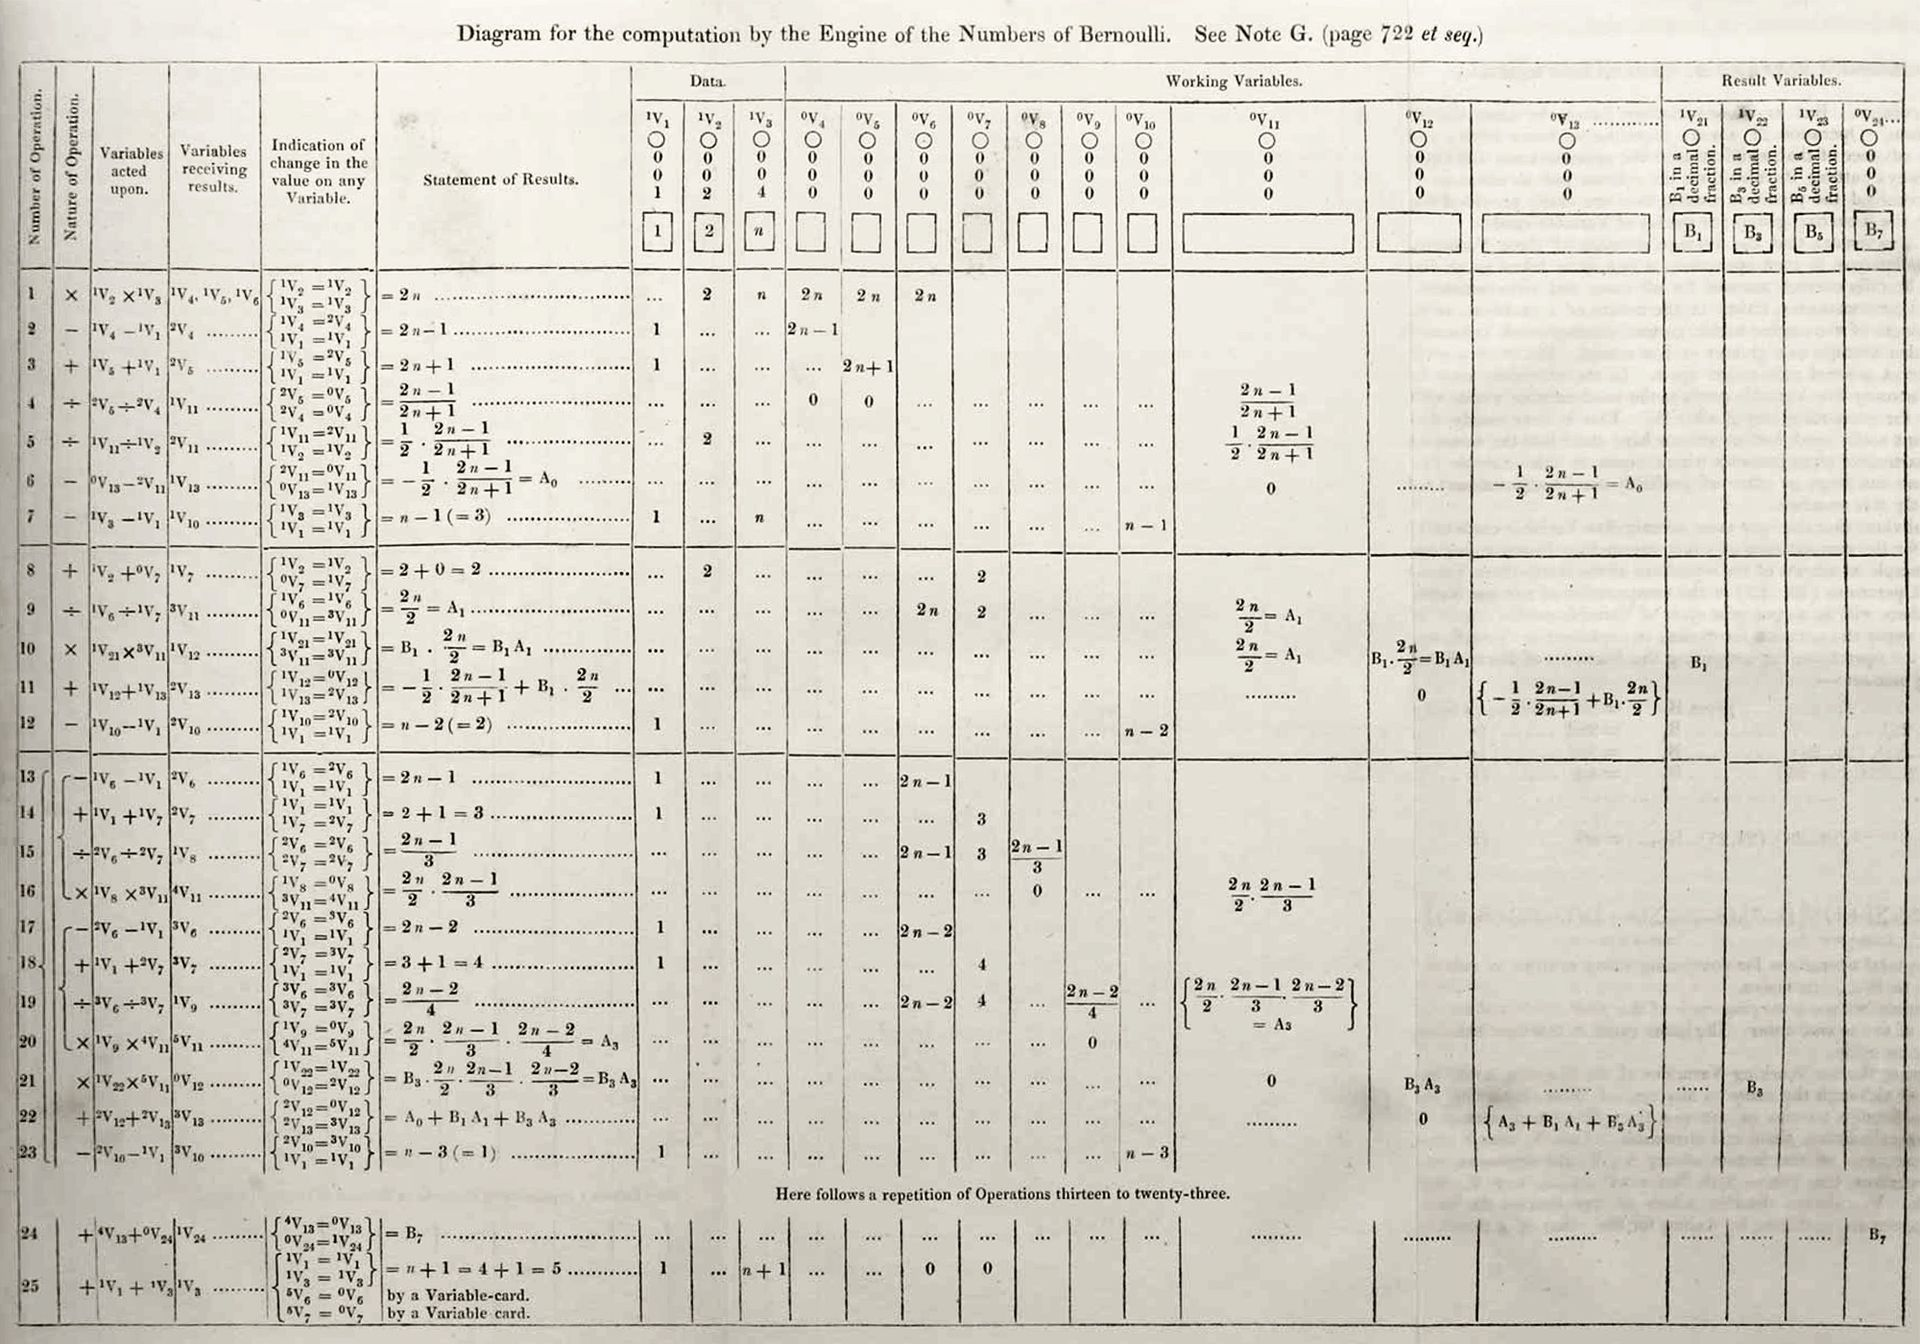
\includegraphics[width=26.67in]{images/algorithm_lovelace} 

}

\caption{El algoritmo diseñado por Ada Lovelace.}\label{fig:unnamed-chunk-55}
\end{figure}

\begin{Shaded}
\begin{Highlighting}[]
\CommentTok{#Código que no funciona porque uno es caracter}
\DecValTok{2} \OperatorTok{+}\StringTok{ "4"} 
\end{Highlighting}
\end{Shaded}

\begin{verbatim}
## Error in 2 + "4": non-numeric argument to binary operator
\end{verbatim}

Si lo piensas, este último error ¡tiene todo el sentido! no puedes sumar un número a un texto. ¿O qué significaría \texttt{\textquotesingle{}Felices\textquotesingle{}\ *\ 4} ?

La magia de \texttt{R} comienza con que puedes almacenar valores en variables. Por ejemplo, podemos asignar un valor a una variable:

\begin{Shaded}
\begin{Highlighting}[]
\CommentTok{#Asignamos x = 10}
\NormalTok{x <-}\StringTok{ }\DecValTok{10}
\end{Highlighting}
\end{Shaded}

Hay dos formas de asignar valores, una es con la flecha de asignación \(\leftarrow\) y otra con el signo de igual:

\begin{Shaded}
\begin{Highlighting}[]
\CommentTok{#Podemos asignar valores con el signo de =}
\NormalTok{y =}\StringTok{ }\DecValTok{6}
\end{Highlighting}
\end{Shaded}

Nota que, cuando realizamos operaciones, la asignación es la última que se realiza:

\begin{Shaded}
\begin{Highlighting}[]
\CommentTok{#Aquí z = 106}
\NormalTok{z <-}\StringTok{ }\NormalTok{y }\OperatorTok{+}\StringTok{ }\NormalTok{x}\OperatorTok{^}\DecValTok{2}
\end{Highlighting}
\end{Shaded}

Los valores que fueron asignados en las variables, \texttt{R} los recuerda y es posible calcular con ellos:

\begin{Shaded}
\begin{Highlighting}[]
\CommentTok{#Podemos realizar una suma}
\NormalTok{x }\OperatorTok{+}\StringTok{ }\NormalTok{y}
\end{Highlighting}
\end{Shaded}

{[}1{]} 16

\begin{Shaded}
\begin{Highlighting}[]
\CommentTok{#O bien podemos realizar una multiplicación}
\DecValTok{3}\OperatorTok{*}\NormalTok{y }\OperatorTok{-}\StringTok{ }\NormalTok{x}
\end{Highlighting}
\end{Shaded}

{[}1{]} 8

Podemos preguntarnos por el valor de las variables numéricas mediante los operadores \texttt{==} (sí, son dos iguales), \texttt{!=} (que es un \(\neq\)) \texttt{\textgreater{}}, \texttt{\textgreater{}=}, \texttt{\textless{}=} y \texttt{\textless{}}:

\begin{Shaded}
\begin{Highlighting}[]
\CommentTok{#Podemos preguntarnos si x vale 4}
\NormalTok{x }\OperatorTok{==}\StringTok{ }\DecValTok{4}
\end{Highlighting}
\end{Shaded}

{[}1{]} FALSE

\begin{quote}
El operador de asignación también se puede utilizar al revés \(2 \rightarrow x\) pero no lo hagas, por favor.
\end{quote}

Nota que no estamos asignando el valor de \texttt{x}:

\begin{Shaded}
\begin{Highlighting}[]
\NormalTok{x}
\end{Highlighting}
\end{Shaded}

{[}1{]} 10

Podemos preguntarnos por diferencia:

\begin{Shaded}
\begin{Highlighting}[]
\NormalTok{x }\OperatorTok{!=}\StringTok{ }\DecValTok{4} 
\end{Highlighting}
\end{Shaded}

{[}1{]} TRUE

Así como por mayores, menores incluyendo posibles igualdades (\emph{i.e.} los casos \(\geq\) y \(\leq\))

\begin{Shaded}
\begin{Highlighting}[]
\CommentTok{#Nos preguntamos si x > y}
\NormalTok{x }\OperatorTok{>}\StringTok{ }\NormalTok{y}
\end{Highlighting}
\end{Shaded}

{[}1{]} TRUE

\begin{Shaded}
\begin{Highlighting}[]
\CommentTok{#Nos preguntamos si x >= 10}
\NormalTok{x }\OperatorTok{>=}\StringTok{ }\DecValTok{10}
\end{Highlighting}
\end{Shaded}

{[}1{]} TRUE

\begin{Shaded}
\begin{Highlighting}[]
\CommentTok{#Nos preguntamos si y < 6}
\NormalTok{y }\OperatorTok{<}\StringTok{ }\DecValTok{6}
\end{Highlighting}
\end{Shaded}

{[}1{]} FALSE

\begin{Shaded}
\begin{Highlighting}[]
\CommentTok{#O bien si y <= 6}
\NormalTok{y }\OperatorTok{<=}\StringTok{ }\DecValTok{6}
\end{Highlighting}
\end{Shaded}

{[}1{]} TRUE

En todos los casos los resultados han sido \texttt{TRUE} ó \texttt{FALSE}. La clase de variables que toma valores \texttt{TRUE} ó \texttt{FALSE} se conoce como booleana. Hay que tener mucho cuidado con ellas porque, puedes acabar con resultados muy extraños:

\begin{Shaded}
\begin{Highlighting}[]
\CommentTok{#MALAS PRÁCTICAS, NO HAGAS ESTO}
\CommentTok{#Cuando lo usas como número TRUE vale 1}
\DecValTok{100} \OperatorTok{+}\StringTok{ }\OtherTok{TRUE}
\end{Highlighting}
\end{Shaded}

{[}1{]} 101

\begin{Shaded}
\begin{Highlighting}[]
\CommentTok{#MALAS PRÁCTICAS, NO HAGAS ESTO}
\CommentTok{#Cuando lo usas como número FALSE vale 0}
\DecValTok{6}\OperatorTok{*}\OtherTok{FALSE}
\end{Highlighting}
\end{Shaded}

{[}1{]} 0

\begin{quote}
\href{https://medium.com/mindorks/common-bad-programming-practices-7fb470ed74d2}{Aquí} puedes encontrar una lista de malas prácticas en computación a evitar.
\end{quote}

Finalmente, nota que es posible reescribir una variable y cambiar su valor:

\begin{Shaded}
\begin{Highlighting}[]
\CommentTok{#Aquí x vale 10, como antes}
\NormalTok{x}
\end{Highlighting}
\end{Shaded}

{[}1{]} 10

\begin{Shaded}
\begin{Highlighting}[]
\CommentTok{#Aquí cambianos el valor de x y valdrá 0.5}
\NormalTok{x <-}\StringTok{ }\FloatTok{0.5}
\NormalTok{x}
\end{Highlighting}
\end{Shaded}

{[}1{]} 0.5

\hypertarget{ejercicios}{%
\subsection{Ejercicios}\label{ejercicios}}

Determina el valor que imprime \texttt{R} en cada caso, sin que corras los siguientes pedazos de código. Después, verifica tu respuesta con \texttt{R}:

\begin{Shaded}
\begin{Highlighting}[]
\CommentTok{#Primer ejercicio}
\NormalTok{x <-}\StringTok{ }\DecValTok{100}
\NormalTok{y <-}\StringTok{ }\DecValTok{3}
\NormalTok{x }\OperatorTok{>}\StringTok{ }\NormalTok{y}
\end{Highlighting}
\end{Shaded}

\begin{Shaded}
\begin{Highlighting}[]
\CommentTok{#Segundo ejercicio}
\NormalTok{z <-}\StringTok{ }\NormalTok{(}\DecValTok{4} \OperatorTok{-}\StringTok{ }\DecValTok{2}\NormalTok{)}\OperatorTok{^}\DecValTok{3}
\NormalTok{z <-}\StringTok{ }\NormalTok{z }\OperatorTok{+}\StringTok{ }\NormalTok{z }\OperatorTok{+}\StringTok{ }\NormalTok{z}
\NormalTok{z}
\end{Highlighting}
\end{Shaded}

\begin{Shaded}
\begin{Highlighting}[]
\CommentTok{#Tercer ejercicio}
\NormalTok{x <-}\StringTok{ }\DecValTok{3}
\NormalTok{y <-}\StringTok{ }\DecValTok{2}
\NormalTok{z <-}\StringTok{ }\NormalTok{x }\OperatorTok{*}\StringTok{ }\NormalTok{y}
\NormalTok{x <-}\StringTok{ }\DecValTok{5}
\NormalTok{y <-}\StringTok{ }\DecValTok{10}
\NormalTok{z}
\end{Highlighting}
\end{Shaded}

\begin{Shaded}
\begin{Highlighting}[]
\CommentTok{#Cuarto ejercicio}
\NormalTok{variable1 <-}\StringTok{ }\DecValTok{1000}
\NormalTok{variable2 <-}\StringTok{ }\DecValTok{100}
\NormalTok{variable3 <-}\StringTok{ }\NormalTok{variable1}\OperatorTok{/}\NormalTok{variable2 }\OperatorTok{<=}\StringTok{ }\DecValTok{10}
\NormalTok{variable3}
\end{Highlighting}
\end{Shaded}

\begin{Shaded}
\begin{Highlighting}[]
\CommentTok{#Quinto ejercicio}
\StringTok{"2"} \OperatorTok{-}\StringTok{ }\DecValTok{2}
\end{Highlighting}
\end{Shaded}

\begin{Shaded}
\begin{Highlighting}[]
\CommentTok{#Sexto ejercicio}
\NormalTok{(}\FloatTok{0.1} \OperatorTok{+}\StringTok{ }\FloatTok{0.1} \OperatorTok{+}\StringTok{ }\FloatTok{0.1}\NormalTok{) }\OperatorTok{==}\StringTok{ }\FloatTok{0.3}
\end{Highlighting}
\end{Shaded}

\hypertarget{nivel-3}{%
\subsection{NIVEL 3}\label{nivel-3}}

Determina, sin correr el programa, qué regresa la consola en este caso

\begin{Shaded}
\begin{Highlighting}[]
\NormalTok{x <-}\StringTok{ }\DecValTok{2} 
\NormalTok{x <-}\StringTok{ }\DecValTok{5} \OperatorTok{+}\StringTok{ }\NormalTok{x ->}\StringTok{ }\NormalTok{y ->}\StringTok{ }\NormalTok{x}
\NormalTok{x <-}\StringTok{ }\NormalTok{x}\OperatorTok{^}\DecValTok{2}
\NormalTok{x}
\end{Highlighting}
\end{Shaded}

Comprueba con la consola tus resultados; puede que encuentres respuestas poco intuitivas.

\hypertarget{observaciones-sobre-la-aritmuxe9tica-de-punto-flotante}{%
\section{Observaciones sobre la aritmética de punto flotante}\label{observaciones-sobre-la-aritmuxe9tica-de-punto-flotante}}

Si hiciste el penúltimo ejercicio (el cual, obviamente hiciste y comprobaste con la consola) podrás haber notado una trampa. Analicemos qué ocurre; quizá hicimos mal la suma

\begin{Shaded}
\begin{Highlighting}[]
\CommentTok{#Veamos si este lado está mal}
\NormalTok{(}\FloatTok{0.1} \OperatorTok{+}\StringTok{ }\FloatTok{0.1} \OperatorTok{+}\StringTok{ }\FloatTok{0.1}\NormalTok{)}
\end{Highlighting}
\end{Shaded}

{[}1{]} 0.3

\begin{Shaded}
\begin{Highlighting}[]
\CommentTok{#O si éste es el que tiene la trampa}
\FloatTok{0.3}
\end{Highlighting}
\end{Shaded}

{[}1{]} 0.3

Aparentemente no hay nada malo ¿qué rayos le pasa a \texttt{R}? La respuesta está \href{https://www.youtube.com/watch?v=PZRI1IfStY0}{en la aritmética de punto flotante}. Podemos pedirle a \texttt{R} que nos muestre los primeros 100 dígitos de la suma \texttt{0.1\ +\ 0.1\ +\ 0.1}:

\begin{figure}

{\centering 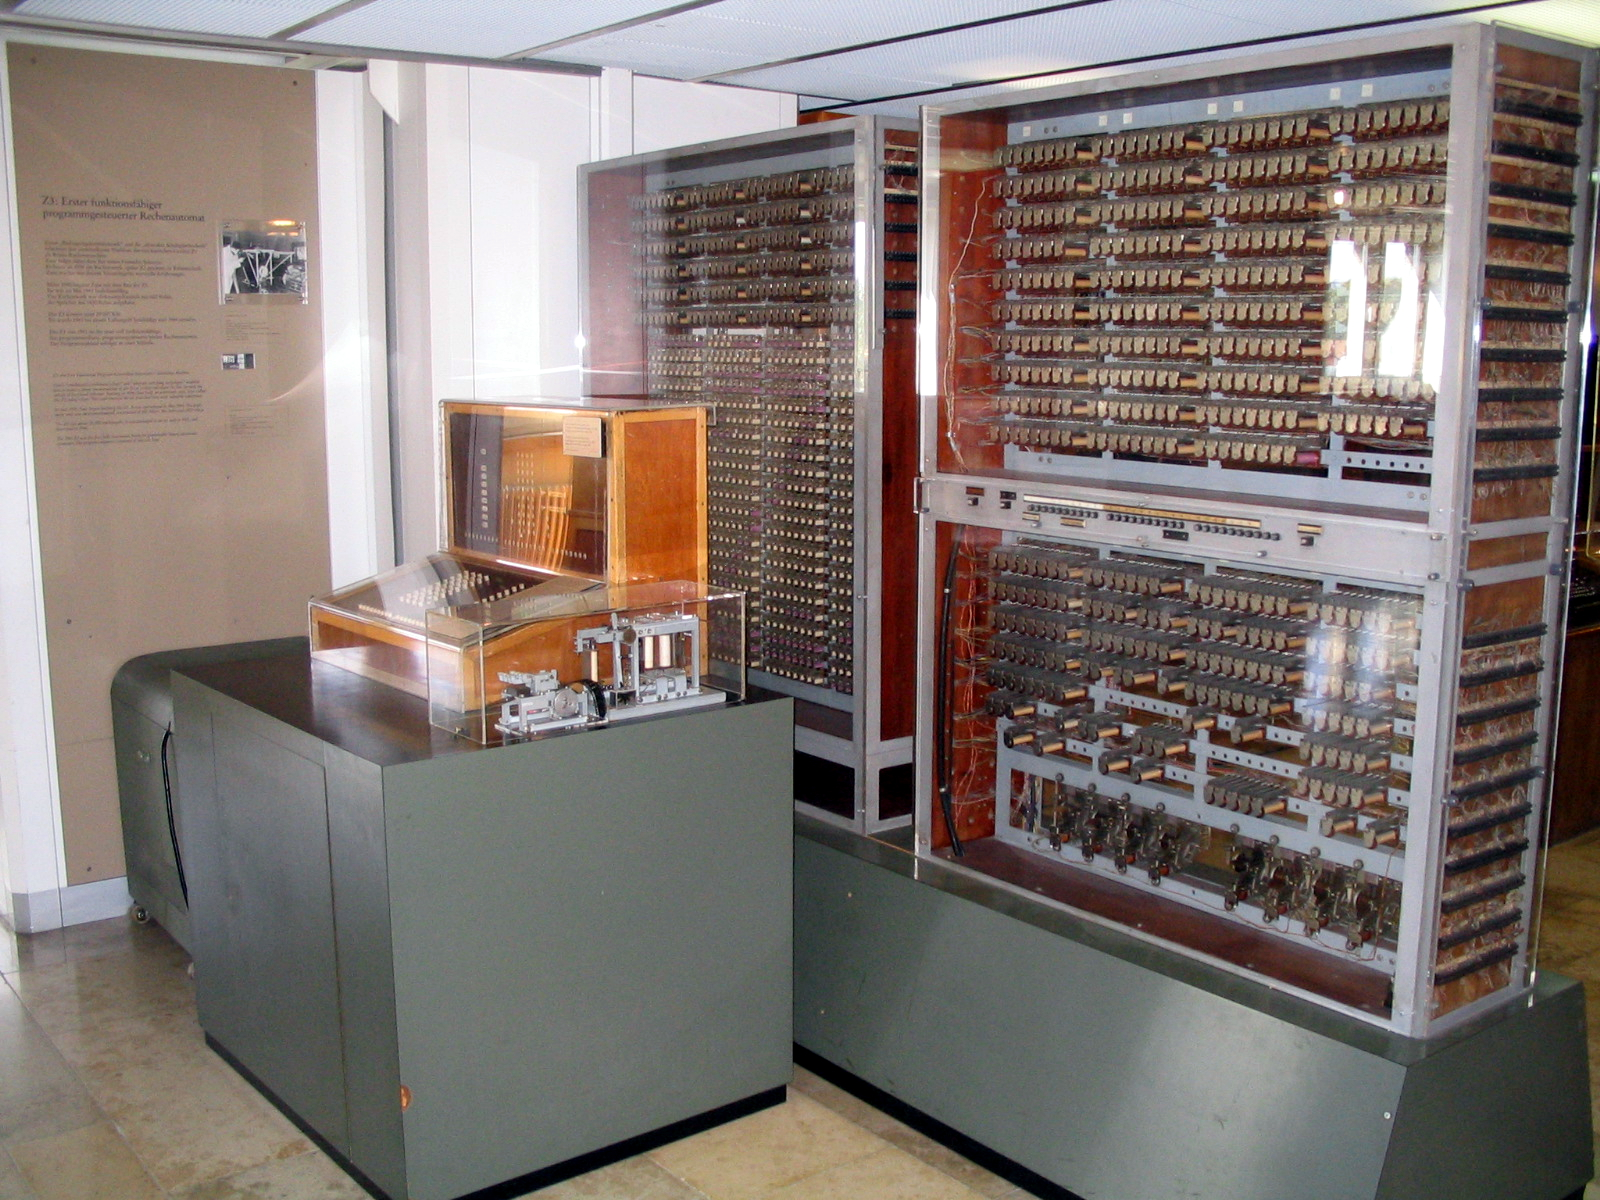
\includegraphics[width=22.22in]{images/Z3_Deutsches_Museum} 

}

\caption{Réplica de la Z3, la primer computadora con punto flotante (1941).}\label{fig:unnamed-chunk-75}
\end{figure}

\begin{Shaded}
\begin{Highlighting}[]
\CommentTok{#Veamos qué pasa con la suma}
\KeywordTok{options}\NormalTok{(}\DataTypeTok{digits =} \DecValTok{22}\NormalTok{) }\CommentTok{#Cambiamos dígitos}
\NormalTok{(}\FloatTok{0.1} \OperatorTok{+}\StringTok{ }\FloatTok{0.1} \OperatorTok{+}\StringTok{ }\FloatTok{0.1}\NormalTok{)    }\CommentTok{#Sumamos}
\end{Highlighting}
\end{Shaded}

{[}1{]} 0.3000000000000000444089

\begin{quote}
El comando \texttt{options(digits\ =\ 22)} especifica que \texttt{R} debe imprimir en la consola \texttt{22} dígitos. No más.
\end{quote}

¡\href{https://www.youtube.com/watch?v=1jaCpeXg-gg}{Ahí está el detalle}! \texttt{R} no sabe sumar. En general, ningún programa de computadora sabe hacerlo. Veamos otros ejemplos:

\begin{Shaded}
\begin{Highlighting}[]
\FloatTok{4.1} \OperatorTok{-}\StringTok{ }\FloatTok{0.1} \CommentTok{#Debería dar 4}
\end{Highlighting}
\end{Shaded}

{[}1{]} 3.999999999999999555911

\begin{Shaded}
\begin{Highlighting}[]
\DecValTok{3}\OperatorTok{/}\DecValTok{10}      \CommentTok{#Debería ser 0.3}
\end{Highlighting}
\end{Shaded}

{[}1{]} 0.2999999999999999888978

\begin{Shaded}
\begin{Highlighting}[]
\KeywordTok{log}\NormalTok{(}\DecValTok{10}\OperatorTok{^}\NormalTok{(}\DecValTok{12345}\NormalTok{), }\DataTypeTok{base =} \DecValTok{10}\NormalTok{) }\CommentTok{#Debería dar 12345}
\end{Highlighting}
\end{Shaded}

{[}1{]} Inf

El problema está en cómo las computadoras representan los números. Ellas escriben los números en binario. Por ejemplo, 230 lo representan como 11100110 mientras que el 7 es: 111. El problema de las computadoras radica en que éstas tienen una memoria finita por lo que números muy grandes como: \(124765731467098372654176\) la computadora hace lo mejor por representarlos eligiendo el más cercano:

\begin{Shaded}
\begin{Highlighting}[]
\CommentTok{#Nota la diferencia entre lo que le decimos a R}
\CommentTok{#y lo que resulta}
\NormalTok{x <-}\StringTok{ }\DecValTok{124765731467098372654176}
\NormalTok{x}
\end{Highlighting}
\end{Shaded}

{[}1{]} 124765731467098377420800

\begin{quote}
Un error de punto flotante en la vida real ocasionó en los años noventa, \href{https://www.esa.int/Newsroom/Press_Releases/Ariane_501_-_Presentation_of_Inquiry_Board_report}{la explosión del cohete \texttt{Ariane\ 5}}. Moraleja: hay que tener cuidado y respeto al punto flotante.
\end{quote}

No olvides cambiar la cantidad de dígitos que deseas que imprima \texttt{R} en su consola de vuelta:

\begin{Shaded}
\begin{Highlighting}[]
\KeywordTok{options}\NormalTok{(}\DataTypeTok{digits =} \DecValTok{6}\NormalTok{) }\CommentTok{#Cambiamos dígitos}
\end{Highlighting}
\end{Shaded}

El mismo problema ocurre con números decimales cuya representación binaria es periódica; por ejemplo el \(\frac{1}{10}\) en binario se representa como \(0.0001100110011\overline{0011}\dots\). Como es el cuento de nunca acabar con dicho número, \texttt{R} lo trunca y almacena sólo los primeros dígitos de ahí que, cada vez que escribes \texttt{0.1}, \texttt{R} en realidad almacene el 0.1000000000000000055511 que es \emph{casi lo mismo} pero no es estrictamente igual. Hay que tener mucho cuidado con esta inexactitud de las computadoras (inexactitud estudiada por la rama de \href{https://www.springer.com/gp/book/9781461484523}{Análisis Numérico}) pues puede generar varios resultados imprevistos.

\hypertarget{cuxf3mo-checar-un-if}{%
\subsection{¿Cómo checar un if?}\label{cuxf3mo-checar-un-if}}

En general lo que hacen las computadoras para comparar valores es que verifican que, en valor absoluto, el error sea pequeño. Recuerda que el valor absoluto de \(x\), \(|x|\), regresa siempre el positivo:
\[
|4| = 4 \qquad \textrm{y} \qquad |-8| = 8
\]

Para verificar que algo es más o menos \(0.3\) suele usarse el valor absoluto\footnote{En \texttt{R} el comando \texttt{abs} toma el valor absoluto.} de la siguiente manera:

\begin{Shaded}
\begin{Highlighting}[]
\KeywordTok{abs}\NormalTok{( (}\FloatTok{0.1} \OperatorTok{+}\StringTok{ }\FloatTok{0.1} \OperatorTok{+}\StringTok{ }\FloatTok{0.1}\NormalTok{) }\OperatorTok{-}\StringTok{ }\FloatTok{0.3}\NormalTok{ ) }\OperatorTok{<}\StringTok{ }\DecValTok{1}\NormalTok{.e}\DecValTok{-6}
\end{Highlighting}
\end{Shaded}

{[}1{]} TRUE

donde \texttt{1.e-6} es notación corta para 0.000001 (también escrito como \(1\times 10^{-6}\)). La pregunta que nos estamos haciendo es que si el error entre sumar \(0.1+0.1+0.1\) y \(0.3\) es muy pequeño \(< 0.000001\):
\[
| (0.1 + 0.1 + 0.1) - 0.3 | < 0.000001
\]

\hypertarget{leer-y-almacenar-variables-en-r}{%
\section{\texorpdfstring{Leer y almacenar variables en \texttt{R}}{Leer y almacenar variables en R}}\label{leer-y-almacenar-variables-en-r}}

Para terminar esta sección, aprenderemos cómo guardar variables en \texttt{R}. Para eso, el concepto de directorio es uno de los más relevantes. En general, en computación, \href{https://en.wikipedia.org/wiki/Working_directory}{el directorio} se refiere a la dirección en tu computadora donde estás trabajando. Por ejemplo, si estás en una carpeta en tu escritorio de nombre ``Ejercicios\_R'' probablemente tu directorio sea `\textasciitilde/Desktop/Ejercicios\_R/' (en Mac) o bien `\textasciitilde\textbackslash Desktop\textbackslash Ejercicios\_R\textbackslash{}' en Windows\footnote{Windows usa backslash. Y hay \href{https://www.howtogeek.com/181774/why-windows-uses-backslashes-and-everything-else-uses-forward-slashes/}{toda una historia detrás de ello}}. La forma de saber tu directorio (en general) es ir a la carpeta que te interesa y con clic derecho ver propiedades (o escribir \texttt{ls} en la terminal \texttt{Unix}).

\texttt{R} tiene un directorio \texttt{default} que quién sabe dónde está (depende de tu instalación, generalmente está donde tu \texttt{Usuario}). Usualmente lo mejor es elegir un directorio para cada uno de los proyectos que hagas. Para ello si estás en \texttt{RStudio} puedes utilizar \texttt{Shift+Ctrl+H} (\texttt{Shift+Cmd+H} en Mac) o bien ir a \texttt{Session\ \textgreater{}\ Set\ Working\ Directory\ \textgreater{}\ Choose\ Directory} y elegir el directorio donde deseas trabajar tu proyecto. Pensando que elegiste el escritorio (\texttt{Desktop} en mi computadora) notarás que en la consola aparece el comando \texttt{setwd("\textasciitilde{}/Desktop")} (o bien con `\textbackslash{}' si eres Windows). Mi sugerencia es que copies ese comando en tu \texttt{Script} para que, la próxima vez que lo corras ya tengas preestablecido el directorio.

\begin{Shaded}
\begin{Highlighting}[]
\CommentTok{#Si eres Mac/Linux}
\KeywordTok{setwd}\NormalTok{(}\StringTok{"~/Desktop"}\NormalTok{) }

\CommentTok{#Si eres Windows}
\KeywordTok{setwd}\NormalTok{(}\StringTok{"C:\textbackslash{}Users\textbackslash{}Rodrigo\textbackslash{}Desktop"}\NormalTok{) }\CommentTok{#Rodrigo = Mi usuario}
\end{Highlighting}
\end{Shaded}

Podemos verificar el directorio elegido con \texttt{getwd()}:

\begin{Shaded}
\begin{Highlighting}[]
\KeywordTok{getwd}\NormalTok{()}
\end{Highlighting}
\end{Shaded}

\begin{quote}
En general es buena práctica en \texttt{R} establecer, hasta arriba del \texttt{Script}, el comando de directorio. Esto con el propósito de que, cuando compartas un archivo, la persona a quien le fue compartido el archivo pueda rápidamente elegir su propio directorio en su computadora.
\end{quote}

Probemos guardar unas variables en un archivo dentro de nuestro directorio. Para ello utilizaremos el comando \texttt{save}.

\begin{Shaded}
\begin{Highlighting}[]
\CommentTok{#Crear las variables}
\NormalTok{x <-}\StringTok{ }\DecValTok{200}
\NormalTok{y <-}\StringTok{ }\DecValTok{100}

\CommentTok{#Los archivos de variables de R son rda}
\KeywordTok{save}\NormalTok{(x,y, }\DataTypeTok{file =} \StringTok{"MisVariables.rda"}\NormalTok{)}
\end{Highlighting}
\end{Shaded}

Si vas a tu directorio, notarás que el archivo \texttt{MisVariables.rda} acaba de ser creado. De esta forma \texttt{R} puede almacenar objetos creados en \texttt{R} que sólo \texttt{R} puede leer (más adelante veremos cómo exportar bases de datos y gráficas). Observa que en tu ambiente (si estás en \texttt{RStudio} puedes verlas en el panel 3) deben aparecer las variables que hemos usado hasta ahora:

{[}1{]} ``x'' ``y'' ``z'' ``tamaño.muestra''
{[}5{]} ``Example1'' ``muestra'' ``pgorro'' ``i''\\
{[}9{]} ``nsim'' ``poblacion'' ``conteo\_rojos''

Podemos probar sumar nuestras variables y todo funciona súper:

\begin{Shaded}
\begin{Highlighting}[]
\NormalTok{x }\OperatorTok{+}\StringTok{ }\NormalTok{y }\CommentTok{#Funciona magníficamente}
\end{Highlighting}
\end{Shaded}

{[}1{]} 300

Limpiemos el ambiente. El comando equivalente al \texttt{clear\ all} en \texttt{R} es un poco más complicado de memorizar:

\begin{Shaded}
\begin{Highlighting}[]
\CommentTok{#EL clear all de R}
\KeywordTok{rm}\NormalTok{(}\DataTypeTok{list =} \KeywordTok{ls}\NormalTok{())}
\end{Highlighting}
\end{Shaded}

Ahora, si vuelves a ver el ambiente, éste estará vacío: ¡hemos limpiado el historial! Nota que si intentamos operar con las variables, \texttt{R} ya no las recuerda:

\begin{Shaded}
\begin{Highlighting}[]
\NormalTok{x }\OperatorTok{+}\StringTok{ }\NormalTok{y }\CommentTok{#Error}
\end{Highlighting}
\end{Shaded}

\begin{verbatim}
## Error in eval(expr, envir, enclos): object 'x' not found
\end{verbatim}

\begin{quote}
Así como hay que lavarse las manos antes de comer, es buen hábito limpiar todas las variables del ambiente de \texttt{R} antes de usarlo.
\end{quote}

Podemos leer la base de datos usando \texttt{load}:

\begin{Shaded}
\begin{Highlighting}[]
\CommentTok{#Leemos las variables}
\KeywordTok{load}\NormalTok{(}\StringTok{"MisVariables.rda"}\NormalTok{)}

\CommentTok{#Una vez leídas podemos empezar a jugar con ellas}
\NormalTok{x }\OperatorTok{+}\StringTok{ }\NormalTok{y }\CommentTok{#Ya funciona}
\end{Highlighting}
\end{Shaded}

{[}1{]} 300

Por último, es necesario resaltar la importancia del directorio. Para ello crea una nueva carpeta en tu escritorio de nombre Mi\_curso\_de\_R. Mueve el archivo \texttt{"MisVariables.rda"} dentro de la carpeta. Borra todo e intenta leer de nuevo el archivo:

\begin{Shaded}
\begin{Highlighting}[]
\CommentTok{#Borramos todo}
\KeywordTok{rm}\NormalTok{(}\DataTypeTok{list =} \KeywordTok{ls}\NormalTok{())}

\CommentTok{#Intentamos leer el archivo de nuevo}
\KeywordTok{load}\NormalTok{(}\StringTok{"MisVariables.rda"}\NormalTok{)}
\end{Highlighting}
\end{Shaded}

Este error es porque \texttt{R} sigue pensando que nuestro directorio es el escritorio y está buscando el archivo ahí sin hallarlo. Para encontrarlo hay que cambiar el directorio a través de \texttt{RStudio} (ya sea \texttt{Ctrl+Shift+H} o \texttt{Session\ \textgreater{}Set\ Working\ Directory\ \textgreater{}\ Choose\ Directory}) o bien a través de comandos en \texttt{R}:

\begin{Shaded}
\begin{Highlighting}[]
\CommentTok{#Si eres Mac/Linux}
\KeywordTok{setwd}\NormalTok{(}\StringTok{"~/Desktop/Mi_curso_de_R"}\NormalTok{) }

\CommentTok{#Si eres Windows}
\KeywordTok{setwd}\NormalTok{(}\StringTok{"C:\textbackslash{}Users\textbackslash{}Rodrigo\textbackslash{}Desktop\textbackslash{}Mi_curso_de_R"}\NormalTok{) }\CommentTok{#Rodrigo = Mi usuario}
\end{Highlighting}
\end{Shaded}

\begin{Shaded}
\begin{Highlighting}[]
\CommentTok{#Aquí sí se puede leer}
\KeywordTok{load}\NormalTok{(}\StringTok{"MisVariables.rda"}\NormalTok{)}
\end{Highlighting}
\end{Shaded}

\hypertarget{ejercicio-2}{%
\subsection{Ejercicio}\label{ejercicio-2}}

Responde a las siguientes preguntas:

\begin{enumerate}
\def\labelenumi{\arabic{enumi}.}
\item
  ¿Qué es el directorio y por qué es necesario establecerlo?
\item
  Si \texttt{R} me da el error \texttt{\textquotesingle{}No\ such\ file\ or\ directory\textquotesingle{}} ¿qué hice mal?
\item
  En \texttt{RStudio}, ¿qué hace \texttt{Session\ \textgreater{}\ Restart\ R}? ¿cuál es la diferencia con \texttt{rm(list\ =\ ls())}?
\item
  ¿Qué hace el comando \texttt{cat("\textbackslash{}014")}? (\emph{Ojo} puede que no haga nada). Si funciona, ¿cuál es la diferencia con \texttt{rm(list\ =\ ls())} y con \texttt{Restart\ R}?
\end{enumerate}

\hypertarget{instalaciuxf3n-de-paquetes}{%
\section{Instalación de paquetes}\label{instalaciuxf3n-de-paquetes}}

Un paquete de \texttt{R} es un conjunto de funciones adicionales elaboradas por los usuarios, las cuales permiten hacer cosas adicionales en \texttt{R}. Para instalarlos requieres de una conexión a Internet (o bien puedes instalarlos a partir de un archivo, por ejemplo, mediante una \texttt{USB}). El comando de instalación es \texttt{install.packages} seguido del nombre del paquete. Por ejemplo (y por ocio) descarguemos el paquete \texttt{beepr} para hacer reproducir sonidos en la computadora\footnote{En los siguientes capítulos descargaremos paquetes más interesantes; pero no desprecies la utilidad de \texttt{beepr} yo lo he usado en múltiples ocasiones para que la computadora me avise que ya terminó de correr un código.}. Para ello:

\begin{Shaded}
\begin{Highlighting}[]
\KeywordTok{install.packages}\NormalTok{(}\StringTok{"beepr"}\NormalTok{)}
\end{Highlighting}
\end{Shaded}

\begin{verbatim}
[...]
* DONE (beepr)

The downloaded source packages are in
    ‘/algun/lugar/downloaded_packages’
\end{verbatim}

Esto significa que el paquete ha sido instalado. Nos interesa usar la función \texttt{beep} que emite un sonido (\texttt{??beep} para ver la ayuda). Si la llamamos así tal cual, nos da error:

\begin{Shaded}
\begin{Highlighting}[]
\KeywordTok{beep}\NormalTok{(}\DecValTok{3}\NormalTok{)}
\end{Highlighting}
\end{Shaded}

\texttt{R} es incapaz de hallar la función porque aún no le hemos dicho dónde se encuentra. Para ello podemos llamar al paquete mediante la función \texttt{library} y decirle a \texttt{R} que incluya las funciones que se encuentran dentro de \texttt{beepr}:

\begin{Shaded}
\begin{Highlighting}[]
\KeywordTok{library}\NormalTok{(beepr)}
\KeywordTok{beep}\NormalTok{(}\DecValTok{3}\NormalTok{) }\CommentTok{#Esto produce un sonido}
\end{Highlighting}
\end{Shaded}

El comando \texttt{library} le dice a \texttt{R} ¡hey, voy a usar unas funciones que creó alguien más y que están dentro del paquete \texttt{beepr}! De esta manera, al correr \texttt{beep(3)}, \texttt{R} ya sabe dónde hallar la función y por eso no arroja error.

\hypertarget{ejercicios-1}{%
\subsection{Ejercicios}\label{ejercicios-1}}

\textbf{NIVEL 1}

\begin{enumerate}
\def\labelenumi{\arabic{enumi}.}
\tightlist
\item
  Instala los paquetes \texttt{tidyverse} en \texttt{R}.
\item
  De \texttt{tidyverse} haz lo necesario para que el siguiente bloque de código te arroje una gráfica:
\end{enumerate}

\begin{Shaded}
\begin{Highlighting}[]
\CommentTok{#Aquí tienes que hacer algo}
\CommentTok{#}
\CommentTok{# RELLENA AQUÍ}
\CommentTok{#}

\CommentTok{#Esto genera un histograma}
\KeywordTok{set.seed}\NormalTok{(}\DecValTok{1364752}\NormalTok{)}
\NormalTok{mis.datos <-}\StringTok{ }\KeywordTok{data.frame}\NormalTok{(}\DataTypeTok{x =} \KeywordTok{rnorm}\NormalTok{(}\DecValTok{1000}\NormalTok{))}
\KeywordTok{ggplot}\NormalTok{(mis.datos, }\KeywordTok{aes}\NormalTok{(}\DataTypeTok{x =}\NormalTok{ x)) }\OperatorTok{+}\StringTok{ }
\StringTok{  }\KeywordTok{geom_histogram}\NormalTok{(}\DataTypeTok{bins =} \DecValTok{50}\NormalTok{, }\DataTypeTok{fill =} \StringTok{"deepskyblue3"}\NormalTok{) }\OperatorTok{+}
\StringTok{  }\KeywordTok{ggtitle}\NormalTok{(}\StringTok{"Histograma generado por el código")}
\end{Highlighting}
\end{Shaded}

\begin{center}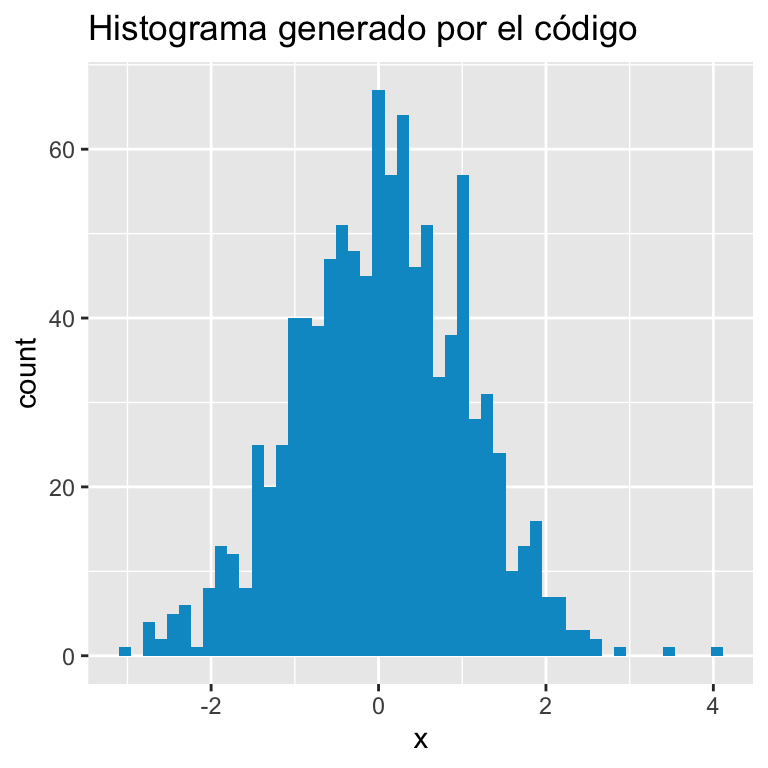
\includegraphics{InferenciaEstadistica_files/figure-latex/unnamed-chunk-98-1} \end{center}

\textbf{NIVEL 3}

\begin{enumerate}
\def\labelenumi{\arabic{enumi}.}
\tightlist
\item
  Instala el paquete \texttt{devtools} (para hacerlo probablemente necesites instalar más cosas en tu computadora; averigua cuáles)
\item
  Usa \texttt{devtools} para instalar el paquete \href{https://github.com/dill/emoGG}{\texttt{emoGG}} desde Github.
\item
  Verifica que tu instalación fue correcta haciendo la siguiente gráfica:
\end{enumerate}

\begin{Shaded}
\begin{Highlighting}[]
\KeywordTok{library}\NormalTok{(emoGG)}
\KeywordTok{ggplot}\NormalTok{(mtcars, }\KeywordTok{aes}\NormalTok{(wt, mpg))}\OperatorTok{+}\StringTok{ }\KeywordTok{geom_emoji}\NormalTok{(}\DataTypeTok{emoji=}\StringTok{"1f697"}\NormalTok{)}
\end{Highlighting}
\end{Shaded}

\begin{center}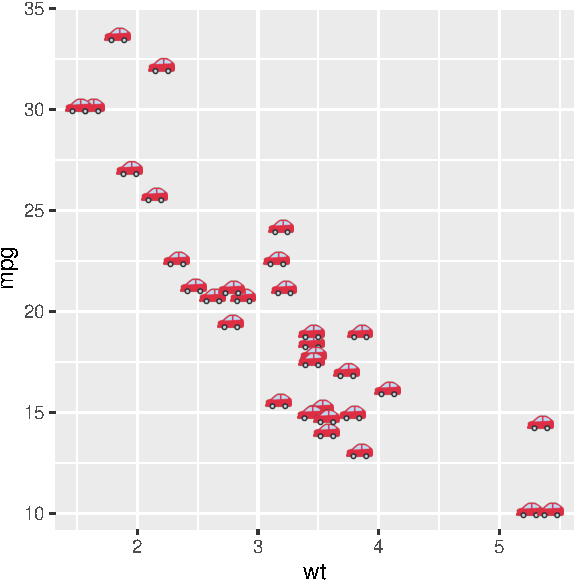
\includegraphics{InferenciaEstadistica_files/figure-latex/unnamed-chunk-99-1} \end{center}

\hypertarget{comentarios-adicionales-sobre-el-formato}{%
\section{Comentarios adicionales sobre el formato}\label{comentarios-adicionales-sobre-el-formato}}

Así como en el español existen reglas de gramática para ponernos todos de acuerdo y entendernos entre todos, en \texttt{R} también existen \emph{sugerencias} a seguir para escribir tu código. Las sugerencias que aquí aparecen fueron adaptadas de las que \href{https://google.github.io/styleguide/Rguide.xml}{utiliza el equipo de \texttt{Google}}.

\begin{enumerate}
\def\labelenumi{\arabic{enumi}.}
\item
  No escribas líneas de más de 80 caracteres (si se salió de tu pantalla, mejor continúa en el siguiente renglón).
\item
  Coloca espacios entre operadores \texttt{+,*,/,-,\textless{}-,=,\ \textless{},\ \textless{}=,\ \textgreater{},\ \textgreater{}=,\ ==} y usa paréntesis para agrupar:
\end{enumerate}

\begin{Shaded}
\begin{Highlighting}[]
\CommentTok{#Esto no se ve muy bien}
\KeywordTok{abs}\NormalTok{(}\DecValTok{3}\OperatorTok{*}\DecValTok{5}\OperatorTok{/}\NormalTok{(}\DecValTok{4-9}\NormalTok{)}\OperatorTok{^}\DecValTok{2-60}\OperatorTok{/}\DecValTok{100-888}\FloatTok{+0.1}\OperatorTok{*}\DecValTok{8888-4}\OperatorTok{/}\DecValTok{10}\OperatorTok{*}\DecValTok{2}\NormalTok{) }\OperatorTok{<}\StringTok{ }\DecValTok{1}\NormalTok{.e}\DecValTok{-6}

\CommentTok{#Los espacios permiten distinguir el orden de las operaciones}
\KeywordTok{abs}\NormalTok{( (}\DecValTok{3} \OperatorTok{*}\StringTok{ }\DecValTok{5}\NormalTok{) }\OperatorTok{/}\StringTok{ }\NormalTok{(}\DecValTok{4} \OperatorTok{-}\StringTok{ }\DecValTok{9}\NormalTok{)}\OperatorTok{^}\DecValTok{2} \OperatorTok{-}\StringTok{ }\DecValTok{60} \OperatorTok{/}\StringTok{ }\DecValTok{100} \OperatorTok{-}\StringTok{ }\DecValTok{888} 
      \OperatorTok{+}\StringTok{ }\NormalTok{(}\FloatTok{0.1} \OperatorTok{*}\StringTok{ }\DecValTok{8888}\NormalTok{) }\OperatorTok{-}\StringTok{ }\NormalTok{(}\DecValTok{4} \OperatorTok{/}\StringTok{ }\DecValTok{10}\NormalTok{) }\OperatorTok{*}\StringTok{ }\DecValTok{2}\NormalTok{ ) }\OperatorTok{<}\StringTok{ }\DecValTok{1}\NormalTok{.e}\DecValTok{-6}
\end{Highlighting}
\end{Shaded}

\begin{enumerate}
\def\labelenumi{\arabic{enumi}.}
\setcounter{enumi}{2}
\tightlist
\item
  Intenta alinear la asignación de variables para legibilidad:
\end{enumerate}

\begin{Shaded}
\begin{Highlighting}[]
\CommentTok{#Esto no tanto}
\NormalTok{altura <-}\StringTok{ }\FloatTok{1.80}
\NormalTok{peso <-}\StringTok{ }\DecValTok{80}
\NormalTok{edad <-}\StringTok{ }\DecValTok{32}

\CommentTok{#Esto se ve bien}
\NormalTok{altura <-}\StringTok{ }\FloatTok{1.80}
\NormalTok{peso   <-}\StringTok{ }\DecValTok{80}
\NormalTok{edad   <-}\StringTok{ }\DecValTok{32}
\end{Highlighting}
\end{Shaded}

\begin{enumerate}
\def\labelenumi{\arabic{enumi}.}
\setcounter{enumi}{3}
\tightlist
\item
  Utiliza nombres que evoquen la variable que representas
\end{enumerate}

\begin{Shaded}
\begin{Highlighting}[]
\CommentTok{#Cuando regreses a esto no sabrás ni qué}
\NormalTok{x <-}\StringTok{ }\DecValTok{10}
\NormalTok{y <-}\StringTok{ }\DecValTok{2}
\NormalTok{z <-}\StringTok{ }\FloatTok{3.14}
\NormalTok{W <-}\StringTok{ }\NormalTok{z }\OperatorTok{*}\StringTok{ }\NormalTok{x}\OperatorTok{^}\NormalTok{y }\CommentTok{#¿Qué calculé?}

\CommentTok{#Es mejor especificar la variable}
\NormalTok{radio        <-}\StringTok{ }\DecValTok{10}
\NormalTok{potencia     <-}\StringTok{ }\DecValTok{2}
\NormalTok{pi_aprox     <-}\StringTok{ }\FloatTok{3.14}
\NormalTok{area_circulo <-}\StringTok{ }\NormalTok{pi_aprox }\OperatorTok{*}\StringTok{ }\NormalTok{radio}\OperatorTok{^}\NormalTok{potencia}
\end{Highlighting}
\end{Shaded}

\begin{enumerate}
\def\labelenumi{\arabic{enumi}.}
\setcounter{enumi}{4}
\tightlist
\item
  No utilices un nombre demasiado similar para cosas diferentes.
\end{enumerate}

\begin{Shaded}
\begin{Highlighting}[]
\CommentTok{#Aquí, seguro eventualmente te vas a equivocar}
\NormalTok{altura <-}\StringTok{ }\DecValTok{10}   \CommentTok{#Altura del edificio}
\NormalTok{Altura <-}\StringTok{ }\FloatTok{1.8}  \CommentTok{#Mi altura}
\NormalTok{ALTURA <-}\StringTok{ }\DecValTok{2000} \CommentTok{#La altitud de la CDMX}

\CommentTok{#Siempre elegir nombres claros, aunque largos}
\NormalTok{altura.edificio <-}\StringTok{ }\DecValTok{10}   \CommentTok{#Altura del edificio}
\NormalTok{altura.Rodrigo  <-}\StringTok{ }\FloatTok{1.8}  \CommentTok{#Mi altura}
\NormalTok{altura.CDMX     <-}\StringTok{ }\DecValTok{2000} \CommentTok{#La altitud de la CDMX}
\end{Highlighting}
\end{Shaded}

\begin{enumerate}
\def\labelenumi{\arabic{enumi}.}
\setcounter{enumi}{5}
\tightlist
\item
  Comenta:
\end{enumerate}

\begin{Shaded}
\begin{Highlighting}[]
\CommentTok{#¿Qué hace esto?}
\NormalTok{x <-}\StringTok{ }\DecValTok{168}
\NormalTok{x <-}\StringTok{ }\NormalTok{x}\OperatorTok{/}\DecValTok{100}
\NormalTok{y <-}\StringTok{ }\FloatTok{71.2}
\KeywordTok{print}\NormalTok{(y}\OperatorTok{/}\NormalTok{x}\OperatorTok{^}\DecValTok{2}\NormalTok{) }
  
\CommentTok{#Es mejor así}
\NormalTok{altura <-}\StringTok{ }\DecValTok{168}        \CommentTok{#en centímetros}
\NormalTok{altura <-}\StringTok{ }\NormalTok{altura}\OperatorTok{/}\DecValTok{100} \CommentTok{#en metros}
\NormalTok{peso   <-}\StringTok{ }\FloatTok{71.2}       \CommentTok{#peso en kg}
\KeywordTok{print}\NormalTok{(peso}\OperatorTok{/}\NormalTok{altura}\OperatorTok{^}\DecValTok{2}\NormalTok{) }\CommentTok{#índice masa corporal}
\end{Highlighting}
\end{Shaded}

\begin{figure}

{\centering 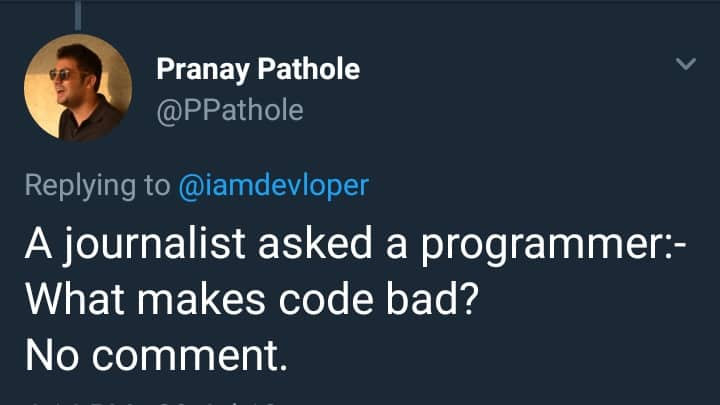
\includegraphics[width=10in]{images/tweet1} 

}

\caption{Trad: Un periodista se acerca a un programador a preguntarle ¿qué hace que un código sea malo? -Sin comentarios.}\label{fig:unnamed-chunk-105}
\end{figure}

\begin{enumerate}
\def\labelenumi{\arabic{enumi}.}
\setcounter{enumi}{6}
\tightlist
\item
  Siempre pon las llamadas a los paquetes y el directorio al inicio de tu archivo para que otro usuario sepa qué necesita.
\end{enumerate}

Código limpio y legible:

\begin{Shaded}
\begin{Highlighting}[]
\CommentTok{#Asumiendo aquí inicia el archivo:}
\KeywordTok{setwd}\NormalTok{(}\StringTok{"Mi directorio"}\NormalTok{)}

\CommentTok{#Llamamos la librería}
\KeywordTok{library}\NormalTok{(beepr)}
\KeywordTok{library}\NormalTok{(tidyverse)}

\CommentTok{#Analizamos una base de datos de R}
\KeywordTok{data}\NormalTok{(iris) }\CommentTok{#Base de datos de flores}

\CommentTok{#Agrupamos la base por especie}
\NormalTok{iris.agrupada <-}\StringTok{ }\KeywordTok{group_by}\NormalTok{(iris, Species)}

\CommentTok{#Obtenemos la media por longitud de sépalo}
\NormalTok{iris.media    <-}\StringTok{ }\KeywordTok{summarise}\NormalTok{(iris.agrupada, }\DataTypeTok{SL.mean =} \KeywordTok{mean}\NormalTok{(Sepal.Length))}

\CommentTok{#Avisa que ya terminó}
\KeywordTok{beep}\NormalTok{(}\DecValTok{5}\NormalTok{)}
\end{Highlighting}
\end{Shaded}

es siempre preferible a código escrito \emph{con prisas} :

\begin{figure}

{\centering 
\includegraphics[width=8.89in]{images/Grandma-Finds-The-Internet} 

}

\caption{Yo, leyendo mi código no comentado y con mala edición 6 meses después de haberlo hecho.}\label{fig:unnamed-chunk-107}
\end{figure}

\begin{Shaded}
\begin{Highlighting}[]
\KeywordTok{data}\NormalTok{(iris);}\KeywordTok{setwd}\NormalTok{(}\StringTok{"Mi directorio"}\NormalTok{)}
\KeywordTok{library}\NormalTok{(tidyverse);x<-}\KeywordTok{group_by}\NormalTok{(iris,Species  )}
\CommentTok{#Aquí hacemos esto}
\NormalTok{iris.means=}\KeywordTok{summarise}\NormalTok{( x,}\DataTypeTok{SL.mean=}\KeywordTok{mean}\NormalTok{(Sepal.Length));}\KeywordTok{library}\NormalTok{(beepr);}\KeywordTok{beep}\NormalTok{(}\DecValTok{5}\NormalTok{)}\CommentTok{#FIN}
\end{Highlighting}
\end{Shaded}

Siempre escribe tu código pensando que alguien más (\href{https://www.redaccionmedica.com/virico/noticias/el-gato-de-schrodinger-y-por-que-no-abrir-la-puerta-cerrada-de-la-consulta-5188}{y ese alguien más puedes ser tú}) va a leerlo. ¡No olvides comentar!

\hypertarget{loops}{%
\section{Loops}\label{loops}}

Vamos a analizar los ciclos (se encuentran en el \href{http://cran.r-project.org/doc/manuals/R-lang.html\#Looping}{manual de R} por si gustas).

\hypertarget{for}{%
\section{For}\label{for}}

Al \texttt{for} lo alimentas con una lista de elementos y él (o ella) realizan la operación indicada con todos los elementos de la lista. Es decir el \texttt{for} recorre de uno por uno los elementos de una lista y les aplica una instrucción.

La estructura es como sigue:
\[
\begin{equation}
\textrm{ for } \Big( \overbrace{i}^\text{Nombre de tu variable} \textrm{ in } \underbrace{1:10}_\text{Lista de elementos}\Big)  \overbrace{ \left \{\textrm{Házle algo a $i$} \right \} }^\text{Instrucción que aplicarle a cada elemento} 
\end{equation}
\]
Por ejemplo una función que imprima los cuadrados de los primeros 10 números:

\begin{Shaded}
\begin{Highlighting}[]
\ControlFlowTok{for}\NormalTok{ (i }\ControlFlowTok{in} \DecValTok{1}\OperatorTok{:}\DecValTok{10}\NormalTok{)\{}
\KeywordTok{print}\NormalTok{(i}\OperatorTok{^}\DecValTok{2}\NormalTok{)}
\NormalTok{\}}
\end{Highlighting}
\end{Shaded}

{[}1{]} 1
{[}1{]} 4
{[}1{]} 9
{[}1{]} 16
{[}1{]} 25
{[}1{]} 36
{[}1{]} 49
{[}1{]} 64
{[}1{]} 81
{[}1{]} 100

\hypertarget{while}{%
\section{While}\label{while}}

El \texttt{while} es una instrucción peligrosa. Un \texttt{while} realiza una instrucción indefinidamente mientras se cumpla una condición. La estructura es como sigue:
\[
\begin{equation}
\textrm{ while } \overbrace{\Big( \textrm{Condición fabulosa} \Big)}^\text{Cosas que tienen que cumplirse para seguir operando} \underbrace{ \left \{ \textrm{Cosas por hacer} \right \}}_\text{Instrucciones}
\end{equation}
\]
Por ejemplo, mientras nuestro número \(i\) sea \(\leq 5\) le sumamos \(1\).
Por ejemplo, mientras nuestro número \(i\) sea \(\leq 5\) le sumamos \(1\).

\begin{Shaded}
\begin{Highlighting}[]
\NormalTok{i=}\DecValTok{1}
\ControlFlowTok{while}\NormalTok{ (i}\OperatorTok{<=}\DecValTok{5}\NormalTok{)\{}
\KeywordTok{print}\NormalTok{(i)}
\NormalTok{i=i}\OperatorTok{+}\DecValTok{1}
\NormalTok{\}}
\end{Highlighting}
\end{Shaded}

\begin{Importante}
Es muy importante que pusiéramos \(i = i + 1\) ya que esto obliga a que
cada vez que da una vuelta la computadora sume el valor de \(i\). Sin
ésta instrucción la \(i\) valdría siempre 1 y jamás saldríamos del loop
(jamás llegaría a valer 5). Si alguna vez quedas atrapado en un loop
puedes usar el botón de STOP que tiene R junto a la consola o la tecla
escape del teclado.
\end{Importante}

\hypertarget{if-else-condicionales}{%
\section{If-else (condicionales)}\label{if-else-condicionales}}

En el manual podemos encontrar la \href{http://cran.r-project.org/doc/manuals/R-lang.html\#if}{sección de condicionales}. Los condicionales evalúan el camino que debe de seguir el código según una condición. Los condicionales tienen la siguiente estructura:

\[
\begin{align*}
if  (Condición)  \left \{  \right. \\ \\ \text{Cosas por hacer si ocurre la condición}  \\ \\ \left.  \right \} else \left \{ \right. \\ \\ \text{Cosas por hacer si no se cumple} \\ \\ \left. \right \} \\ \\
\end{align*}
\]

¡Vamos al ejemplo!

Asignemos, primero, el valor de 2 a \(i\):

\begin{Shaded}
\begin{Highlighting}[]
\NormalTok{i =}\StringTok{ }\DecValTok{2}
\end{Highlighting}
\end{Shaded}

Luego pongamos el condicional

\begin{Shaded}
\begin{Highlighting}[]
\ControlFlowTok{if}\NormalTok{ (i }\OperatorTok{==}\StringTok{ }\DecValTok{5}\NormalTok{)\{   }\CommentTok{# Nota el doble signo de igual '=='. }
\NormalTok{  i=i}\OperatorTok{^}\DecValTok{2}        \CommentTok{# Si sólo pones uno, R hace que i=5.}
\NormalTok{\}}
\end{Highlighting}
\end{Shaded}

Veamos cuánto vale \(i\)

\begin{Shaded}
\begin{Highlighting}[]
\KeywordTok{print}\NormalTok{(i)}
\end{Highlighting}
\end{Shaded}

{[}1{]} 10

Hagamos ahora \(i = 5\) y veamos qué pasa cuando atraviesa el condicional:

\begin{Shaded}
\begin{Highlighting}[]
\NormalTok{i =}\StringTok{ }\DecValTok{5}
\ControlFlowTok{if}\NormalTok{ (i }\OperatorTok{==}\StringTok{ }\DecValTok{5}\NormalTok{)\{   }
\NormalTok{  i=i}\OperatorTok{^}\DecValTok{2}      
\NormalTok{\}}
\KeywordTok{print}\NormalTok{(i)}
\end{Highlighting}
\end{Shaded}

{[}1{]} 25

Hagamos ahora un condicional más complicado: pongamos que si \(i = 5\) entonces haga \(i^2\) pero si \(i \neq 5\) entonces al valor de \(i\) le sume \(1\):

\begin{Shaded}
\begin{Highlighting}[]
\NormalTok{i=}\DecValTok{1}
\ControlFlowTok{if}\NormalTok{ (i }\OperatorTok{==}\StringTok{ }\DecValTok{5}\NormalTok{)\{}
\NormalTok{  i=i}\OperatorTok{^}\DecValTok{2}
\NormalTok{\} }\ControlFlowTok{else}\NormalTok{ \{}
\NormalTok{  i=i}\OperatorTok{+}\DecValTok{1}
\NormalTok{\}}
\KeywordTok{print}\NormalTok{(i)}
\end{Highlighting}
\end{Shaded}

{[}1{]} 2

\hypertarget{and-or-operadores-luxf3gicos}{%
\section{And-or (Operadores lógicos)}\label{and-or-operadores-luxf3gicos}}

¿Qué pasa si tienes varias condiciones que necesitas se cumplan a la vez? ¡Para eso están los \href{http://cran.r-project.org/doc/manuals/R-lang.html\#Operators}{operadores lógicos}! .

\hypertarget{and}{%
\subsection{And}\label{and}}

Por ejemplo, supongamos queremos usar dos condiciones dentro del \texttt{if}. ¡Es muy fácil! Basta con escribir \texttt{Condición} 1 \& \texttt{Condición} 2.

Ejemplo:

\begin{Shaded}
\begin{Highlighting}[]
\NormalTok{i=}\DecValTok{1}
\NormalTok{j=}\DecValTok{7}
\ControlFlowTok{if}\NormalTok{( (i }\OperatorTok{==}\StringTok{ }\DecValTok{1}\NormalTok{) }\OperatorTok{&}\StringTok{ }\NormalTok{(i }\OperatorTok{<}\StringTok{ }\NormalTok{j) ) \{}
\NormalTok{  i=i}\OperatorTok{+}\NormalTok{j  }
\NormalTok{\}}
\KeywordTok{print}\NormalTok{(i)}
\end{Highlighting}
\end{Shaded}

{[}1{]} 8

Por otro lado si ahora hacemos \(i > j\):

\begin{Shaded}
\begin{Highlighting}[]
\NormalTok{i=}\DecValTok{11}
\NormalTok{j=}\DecValTok{7}
\ControlFlowTok{if}\NormalTok{( (i }\OperatorTok{==}\StringTok{ }\DecValTok{1}\NormalTok{) }\OperatorTok{&}\StringTok{ }\NormalTok{(i }\OperatorTok{<}\StringTok{ }\NormalTok{j) ) \{}
\NormalTok{  i=i}\OperatorTok{+}\NormalTok{j  }
\NormalTok{\}}
\KeywordTok{print}\NormalTok{(i)}
\end{Highlighting}
\end{Shaded}

{[}1{]} 11

Y si hacemos que \(i = 1\) pero \(i > j\):

\begin{Shaded}
\begin{Highlighting}[]
\NormalTok{i=}\DecValTok{1}
\NormalTok{j=}\DecValTok{0}
\ControlFlowTok{if}\NormalTok{( (i }\OperatorTok{==}\StringTok{ }\DecValTok{1}\NormalTok{) }\OperatorTok{&}\StringTok{ }\NormalTok{(i }\OperatorTok{<}\StringTok{ }\NormalTok{j) ) \{}
\NormalTok{  i=i}\OperatorTok{+}\NormalTok{j  }
\NormalTok{\}}
\KeywordTok{print}\NormalTok{(i)}
\end{Highlighting}
\end{Shaded}

{[}1{]} 1

\hypertarget{or}{%
\section{Or}\label{or}}

El \texttt{or} se usa en el caso de que querramos que se cumpla al menos una de dos condiciones del \texttt{if}. Es decir, si tenemos dos condiciones el or se cumple cuando se cumple una de ellas o cuando se cumplen ambas. Por ejemplo:

Cuando \(i = 1\) con \(i > j\):

\begin{Shaded}
\begin{Highlighting}[]
\NormalTok{i=}\DecValTok{1}
\NormalTok{j =}\StringTok{ }\DecValTok{1}\OperatorTok{/}\DecValTok{2}
\ControlFlowTok{if}\NormalTok{( (i }\OperatorTok{==}\StringTok{ }\DecValTok{1}\NormalTok{) }\OperatorTok{|}\StringTok{ }\NormalTok{(i }\OperatorTok{<}\StringTok{ }\NormalTok{j) ) \{}
\NormalTok{i=i}\OperatorTok{+}\NormalTok{j}
\NormalTok{\}}
\KeywordTok{print}\NormalTok{(i)}
\end{Highlighting}
\end{Shaded}

{[}1{]} 1.5

Cuando \(i \neq 1\) pero \(i < j\):

\begin{Shaded}
\begin{Highlighting}[]
\NormalTok{i=}\DecValTok{21}
\NormalTok{j =}\StringTok{ }\DecValTok{22}
\ControlFlowTok{if}\NormalTok{( (i }\OperatorTok{==}\StringTok{ }\DecValTok{1}\NormalTok{) }\OperatorTok{|}\StringTok{ }\NormalTok{(i }\OperatorTok{<}\StringTok{ }\NormalTok{j) ) \{}
\NormalTok{i=i}\OperatorTok{+}\NormalTok{j}
\NormalTok{\}}
\KeywordTok{print}\NormalTok{(i)}
\end{Highlighting}
\end{Shaded}

{[}1{]} 43

O bien cuando \(i \neq 1\) e \(i > j\)

\begin{Shaded}
\begin{Highlighting}[]
\NormalTok{i=}\DecValTok{121}
\NormalTok{j =}\StringTok{ }\DecValTok{22}
\ControlFlowTok{if}\NormalTok{( (i }\OperatorTok{==}\StringTok{ }\DecValTok{1}\NormalTok{) }\OperatorTok{|}\StringTok{ }\NormalTok{(i }\OperatorTok{<}\StringTok{ }\NormalTok{j) ) \{}
\NormalTok{i=i}\OperatorTok{+}\NormalTok{j}
\NormalTok{\}}
\KeywordTok{print}\NormalTok{(i)}
\end{Highlighting}
\end{Shaded}

{[}1{]} 121

La siguiente tabla resume cuándo se cumplen las condiciones:

\[
\begin{array}{ccccc} 
Condición 1 & Condición 2 & And & Or \\
\hline
Si & Si & Si & Si \\ 
Si & No & No & Si \\ 
No & Si & No & Si \\ 
No & No & No & No \\ 
\end{array}
\]

\hypertarget{ejercicio-1-1}{%
\section{Ejercicio 1}\label{ejercicio-1-1}}

Crea los comandos necesarios para calcular la media y desviacion estandar del siguiente vector:

\begin{Shaded}
\begin{Highlighting}[]
\NormalTok{numeros <-}\StringTok{ }\KeywordTok{c}\NormalTok{(}\FloatTok{7.65688984}\NormalTok{, }\FloatTok{0.45416281}\NormalTok{, }\FloatTok{-0.53197482}\NormalTok{, }\FloatTok{-11.68901517}\NormalTok{, }
             \FloatTok{-0.22092715}\NormalTok{, }\FloatTok{-6.65860576}\NormalTok{, }\FloatTok{-0.96411401}\NormalTok{, }\FloatTok{-0.04875882}\NormalTok{, }
             \FloatTok{-0.88076032}\NormalTok{, }\FloatTok{-9.47716275}\NormalTok{, }\FloatTok{12.48699956}\NormalTok{, }\FloatTok{58.37690942}\NormalTok{, }
             \FloatTok{0.75332369}\NormalTok{, }\FloatTok{-0.07644519}\NormalTok{, }\FloatTok{-0.47168251}\NormalTok{, }\FloatTok{0.04574367}\NormalTok{, }
             \FloatTok{0.21158367}\NormalTok{, }\FloatTok{6.57919350}\NormalTok{, }\FloatTok{1.61654489}\NormalTok{, }\FloatTok{-144.28602691}\NormalTok{)}
\end{Highlighting}
\end{Shaded}

Tus resultados deberían ser:
{[}1{]} ``Media: -4.356206118''
{[}1{]} ``Desviación: 35.8220144835353''

\texttt{Nota} Para el ejercicio puedes usar cualquier función de R excepto: \texttt{mean}, \texttt{sd}, \texttt{var}.

\begin{Recuadro}
Por si no lo recuerdas, aquí están las definiciones de media y
desviacion estándar. Si bien no es la única forma pues ¡hay varias
definiciones equivalentes!.
\end{Recuadro}

\hypertarget{media}{%
\section{Media}\label{media}}

\[
\begin{equation}
\textrm{Media de }X = \frac{x_1 + x_2 + \cdots + x_n}{n} 
\end{equation}
\]

\hypertarget{desviaciuxf3n-estuxe1ndar}{%
\section{Desviación estándar}\label{desviaciuxf3n-estuxe1ndar}}

\[
\begin{equation}
\textrm{Desviación Estándar de }X = \sqrt{\textrm{Media de }X^2 - \Big(\textrm{Media de }X\Big)^2} 
\end{equation}
\]

\hypertarget{ejercicio-2-1}{%
\section{Ejercicio 2}\label{ejercicio-2-1}}

Sin correr el siguiente pedazo de código en R, estima cuánto valdrá \(k\) al final:

\begin{Shaded}
\begin{Highlighting}[]
\NormalTok{k <-}\StringTok{ }\DecValTok{3}
\ControlFlowTok{for}\NormalTok{ (i }\ControlFlowTok{in} \DecValTok{1}\OperatorTok{:}\DecValTok{6}\NormalTok{)\{}
  
  \ControlFlowTok{if}\NormalTok{ (i }\OperatorTok{>}\StringTok{ }\NormalTok{k }\OperatorTok{||}\StringTok{ }\NormalTok{k }\OperatorTok{==}\StringTok{ }\DecValTok{3}\NormalTok{)\{}
    
\NormalTok{    k <-}\StringTok{ }\NormalTok{k}\OperatorTok{^}\DecValTok{2}
    
\NormalTok{  \} }\ControlFlowTok{else} \ControlFlowTok{if}\NormalTok{ (i }\OperatorTok{==}\StringTok{ }\DecValTok{3} \OperatorTok{&}\StringTok{ }\NormalTok{k }\OperatorTok{==}\StringTok{ }\DecValTok{7}\NormalTok{) \{}
    
\NormalTok{    k <-}\StringTok{ }\NormalTok{k }\OperatorTok{-}\StringTok{ }\DecValTok{2}
    
\NormalTok{  \} }\ControlFlowTok{else} \ControlFlowTok{if}\NormalTok{ (k }\OperatorTok{>}\StringTok{ }\NormalTok{i }\OperatorTok{&}\StringTok{ }\NormalTok{i }\OperatorTok{<}\StringTok{ }\DecValTok{5}\NormalTok{) \{}
    
\NormalTok{    k <-}\StringTok{ }\NormalTok{k}\OperatorTok{*}\NormalTok{i}\OperatorTok{/}\DecValTok{2}
    
\NormalTok{  \} }\ControlFlowTok{else} \ControlFlowTok{if}\NormalTok{ (k }\OperatorTok{>}\StringTok{ }\NormalTok{i }\OperatorTok{&}\StringTok{ }\NormalTok{i }\OperatorTok{>=}\StringTok{ }\DecValTok{5}\NormalTok{) \{}
    
\NormalTok{    k <-}\StringTok{ }\NormalTok{k }\OperatorTok{+}\StringTok{ }\DecValTok{1}
    
\NormalTok{  \} }\ControlFlowTok{else}\NormalTok{ \{}
    
\NormalTok{    k <-}\StringTok{ }\NormalTok{k}\OperatorTok{/}\DecValTok{2}
    
\NormalTok{  \}}
  
\NormalTok{\}}
\end{Highlighting}
\end{Shaded}

\hypertarget{ejercicio-3}{%
\section{Ejercicio 3}\label{ejercicio-3}}

Un grupo de investigadores tienen tres vectores de datos sobre individuos: \texttt{sexo}, \texttt{edad} y exposición (horas) a humo de tabaco \texttt{expo}.

\begin{Shaded}
\begin{Highlighting}[]
\NormalTok{sexo <-}\StringTok{ }\KeywordTok{c}\NormalTok{(}\StringTok{"Hombre"}\NormalTok{,}\StringTok{"Mujer"}\NormalTok{,}\StringTok{"Mujer"}\NormalTok{,}\StringTok{"Mujer"}\NormalTok{,}\StringTok{"Hombre"}\NormalTok{,}
          \StringTok{"Mujer"}\NormalTok{,}\StringTok{"Hombre"}\NormalTok{,}\StringTok{"Hombre"}\NormalTok{)}
\NormalTok{edad <-}\StringTok{ }\KeywordTok{c}\NormalTok{(}\DecValTok{28}\NormalTok{, }\DecValTok{12}\NormalTok{, }\DecValTok{77}\NormalTok{, }\DecValTok{32}\NormalTok{, }\DecValTok{46}\NormalTok{, }\DecValTok{53}\NormalTok{, }\DecValTok{17}\NormalTok{, }\DecValTok{20}\NormalTok{, }\DecValTok{88}\NormalTok{)}
\NormalTok{expo  <-}\StringTok{ }\KeywordTok{c}\NormalTok{(}\DecValTok{1}\NormalTok{, }\DecValTok{0}\NormalTok{, }\FloatTok{1.5}\NormalTok{, }\FloatTok{2.2}\NormalTok{, }\DecValTok{2}\NormalTok{, }\DecValTok{5}\NormalTok{, }\FloatTok{1.01}\NormalTok{, }\FloatTok{3.2}\NormalTok{)}
\end{Highlighting}
\end{Shaded}

Ellos saben que por cada hora de exposición el riesgo relativo de enfermedad cardiovascular es de \(1.025\) para hombres menores a 45 y \(1.032\) para mujeres de la misma edad. Para mayores de 45, el riesgo es \(1.052\) en caso de hombres y \(1.066\) en caso de mujeres.

Los investigadores hicieron el siguiente código para estimar los riesgos de cada uno de los individuos. Ayúdalos a que su código funcione:

\begin{Shaded}
\begin{Highlighting}[]
\CommentTok{#Hay n personas: para cada una hay que calcular su riesgo }

\NormalTok{n      <-}\StringTok{ }\KeywordTok{length}\NormalTok{(sexo)}
\NormalTok{riesgo <-}\StringTok{ }\KeywordTok{c}\NormalTok{()}
\ControlFlowTok{while}\NormalTok{ (persona }\OperatorTok{<}\StringTok{ }\NormalTok{n)\{}
  
  \CommentTok{#Checar la edad de la persona}
  \ControlFlowTok{if}\NormalTok{ (edad[persona] }\OperatorTok{<}\StringTok{ }\DecValTok{45}\NormalTok{)\{}
    
    \CommentTok{#Checar el sexo}
    \ControlFlowTok{if}\NormalTok{ (sexo[persona] =}\StringTok{ }\NormalTok{Hombre)\{}
      
\NormalTok{      riesgo[persona] <-}\StringTok{ }\NormalTok{expo[persona]}\OperatorTok{*}\FloatTok{1.025}
      
\NormalTok{    \} }\ControlFlowTok{else}\NormalTok{ \{}
      
\NormalTok{      riesgo[persona] <-}\StringTok{ }\NormalTok{expo[persona]}\OperatorTok{*}\FloatTok{1.032}
      
\NormalTok{    \}}
    
\NormalTok{  \} }\ControlFlowTok{else}\NormalTok{ \{}
    
    \CommentTok{#Checar el sexo}
    \ControlFlowTok{if}\NormalTok{ (sexo[persona] =}\StringTok{ }\NormalTok{Hombre)\{}
      
\NormalTok{      riesgo[persona] <-}\StringTok{ }\NormalTok{expo[persona]}\OperatorTok{*}\FloatTok{1.052}
      
\NormalTok{    \} }\ControlFlowTok{else}\NormalTok{ \{}
      
\NormalTok{      riesgo[persona] <-}\StringTok{ }\NormalTok{expo[persona]}\OperatorTok{*}\FloatTok{1.066}
      
\NormalTok{    \}}
    
\NormalTok{  \}}
  
  
  
\NormalTok{\}}
\end{Highlighting}
\end{Shaded}

Para que cheques que funcione, te dejo la respuesta. El riesgo es:

{[}1{]} 1.02500 0.00000 1.59900 2.27040 2.10400 5.33000 1.03525

\hypertarget{advertencias-y-otras-cosas-poco-intuitivas}{%
\section{Advertencias y otras cosas poco intuitivas}\label{advertencias-y-otras-cosas-poco-intuitivas}}

Es importante entender cómo funcionan las computadoras para poder simular (y entender los problemas de la simulación). Aunque los números son infinitos, las computadoras no tienen una cantidad infinita de dígitos. Por ejemplo, nosotros (humanos) podemos representar:
\[
\begin{equation}
1 - 0.000000001 = 0.99999999
\end{equation}
\]
La computadora no puede hacerlo:

\begin{Shaded}
\begin{Highlighting}[]
\DecValTok{1} \OperatorTok{-}\StringTok{ }\FloatTok{0.000000001}
\end{Highlighting}
\end{Shaded}

{[}1{]} 1

Tampoco puede representar números muy grandes:

\begin{Shaded}
\begin{Highlighting}[]
\KeywordTok{exp}\NormalTok{(}\DecValTok{1000}\NormalTok{)}
\end{Highlighting}
\end{Shaded}

{[}1{]} Inf

Mientras que para los humanos no hay ``un número positivo más chico'' (si dices, por ejemplo, que \(0.00000000001\) es el más chico de todos los positivos (no cero), siempre puedes dividirlo entre \(2\): \(0.00000000001/2\) y obtener un número más pequeño) para las computadoras sí hay. Eso quiere decir que cuando hacemos una operación la computadora NO da la respuesta correcta sólo su mejor aproximación. A veces su mejor aproximación es la respuesta correcta:

\begin{Shaded}
\begin{Highlighting}[]
\KeywordTok{sqrt}\NormalTok{(}\DecValTok{100}\NormalTok{)}
\end{Highlighting}
\end{Shaded}

{[}1{]} 10

Otras veces está cerca:

\begin{Shaded}
\begin{Highlighting}[]
\KeywordTok{sqrt}\NormalTok{(}\FloatTok{12345678.12345678}\OperatorTok{^}\DecValTok{2}\NormalTok{)}
\end{Highlighting}
\end{Shaded}

{[}1{]} 12345678

Pero\ldots{}

\hypertarget{donde-fallan-estas-cosas}{%
\section{Donde fallan estas cosas}\label{donde-fallan-estas-cosas}}

Intuitivamente, los decimales que nos acabamos de comer en el inciso anterior no importan ¡son simples decimales! El siguiente ejemplo muestra que sí importan.

Este ejemplo calcula una función recursivamente. ¿Puedes explicar qué estamos haciendo?

\begin{Shaded}
\begin{Highlighting}[]
\NormalTok{ejemplo <-}\StringTok{ }\KeywordTok{c}\NormalTok{()}
\NormalTok{a       <-}\StringTok{ }\FloatTok{2.701}
\ControlFlowTok{for}\NormalTok{ (i }\ControlFlowTok{in} \DecValTok{1}\OperatorTok{:}\DecValTok{100}\NormalTok{)\{}
  
  \ControlFlowTok{if}\NormalTok{ (i }\OperatorTok{==}\StringTok{ }\DecValTok{1}\NormalTok{)\{}
    
\NormalTok{    ejemplo[i] <-}\StringTok{ }\DecValTok{10}
    
\NormalTok{  \} }\ControlFlowTok{else}\NormalTok{ \{}
    
\NormalTok{    ejemplo[i] <-}\StringTok{ }\NormalTok{ejemplo[i}\DecValTok{-1}\NormalTok{] }\OperatorTok{+}\StringTok{ }
\StringTok{                  }\NormalTok{a}\OperatorTok{*}\NormalTok{ejemplo[i}\DecValTok{-1}\NormalTok{]}\OperatorTok{*}\NormalTok{(}\DecValTok{1}\OperatorTok{-}\NormalTok{ejemplo[i}\DecValTok{-1}\NormalTok{]}\OperatorTok{/}\DecValTok{100}\NormalTok{)}
    
\NormalTok{  \}}
  
\NormalTok{\}}
 
\KeywordTok{print}\NormalTok{(ejemplo[}\DecValTok{100}\NormalTok{])}
\end{Highlighting}
\end{Shaded}

{[}1{]} 125.863

El ejemplo anterior resulta en un maravilloso resultado de ejemplo{[}100{]}. Redondeemos a dos decimales el valor de \(a\) para que sea \(2.70\). Intuitivamente, el valor debería estar cerca y ser ciento y tantos. Pues no\ldots{}

\begin{Shaded}
\begin{Highlighting}[]
\NormalTok{ejemplo2 <-}\StringTok{ }\KeywordTok{c}\NormalTok{()}
\NormalTok{a       <-}\StringTok{ }\FloatTok{2.70}
\ControlFlowTok{for}\NormalTok{ (i }\ControlFlowTok{in} \DecValTok{1}\OperatorTok{:}\DecValTok{100}\NormalTok{)\{}
  
  \ControlFlowTok{if}\NormalTok{ (i }\OperatorTok{==}\StringTok{ }\DecValTok{1}\NormalTok{)\{}
    
\NormalTok{    ejemplo2[i] <-}\StringTok{ }\DecValTok{10}
    
\NormalTok{  \} }\ControlFlowTok{else}\NormalTok{ \{}
    
\NormalTok{    ejemplo2[i] <-}\StringTok{ }\NormalTok{ejemplo2[i}\DecValTok{-1}\NormalTok{] }\OperatorTok{+}\StringTok{ }
\StringTok{                   }\NormalTok{a}\OperatorTok{*}\NormalTok{ejemplo2[i}\DecValTok{-1}\NormalTok{]}\OperatorTok{*}\NormalTok{(}\DecValTok{1}\OperatorTok{-}\NormalTok{ejemplo2[i}\DecValTok{-1}\NormalTok{]}\OperatorTok{/}\DecValTok{100}\NormalTok{)}
    
\NormalTok{  \}}
  
\NormalTok{\}}
 
\KeywordTok{print}\NormalTok{(ejemplo2[}\DecValTok{100}\NormalTok{])}
\end{Highlighting}
\end{Shaded}

{[}1{]} 87.0938

¡Resulta que con cambiar un decimal, el resultado cambió hasta ejemplo2{[}100{]}!
La gráfica siguiente muestra como varían los valores coincidiendo al inicio y alejándose después:

\begin{center}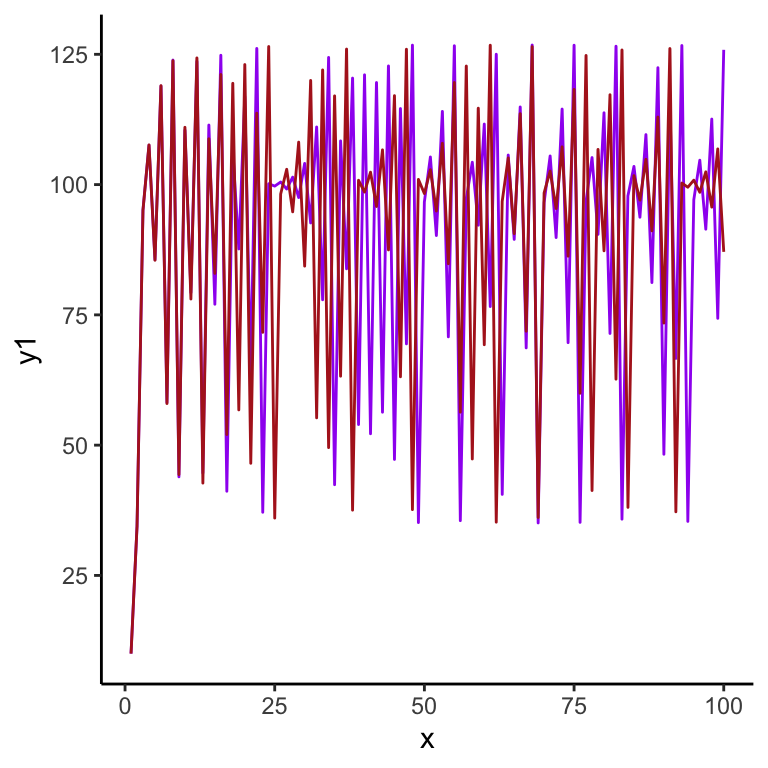
\includegraphics{InferenciaEstadistica_files/figure-latex/unnamed-chunk-136-1} \end{center}

\hypertarget{nuxfameros-pseudoaleatorios}{%
\section{Números pseudoaleatorios}\label{nuxfameros-pseudoaleatorios}}

Para simular necesitamos generar números aleatorios. La única forma que tenemos de hacerlo (actualmente) es por medio de isótopos radiactivos que decaen aleatoriamente. ¡Si tienes uno guardado por ahí es el momento de usarlo!

Como no es muy bueno que tengamos por ahí material radiactivo, los matemáticos han generado números que se conocen como pseudoaleatorios. Estas son funciones (como la del apartado anterior) que si conoces el valor inicial (en el caso pasado, \(a\)) las funciones son tan alocadas que los números que resultan de ella `'parecen aleatorios''.

\hypertarget{ejercicio-4}{%
\section{Ejercicio 4}\label{ejercicio-4}}

Considera los siguientes dos fragmentos de código. Analiza los resultados. ¿Cuál de ellos es un mejor generador pseudoaleatorio y por qué?

\begin{Shaded}
\begin{Highlighting}[]
\NormalTok{a         <-}\StringTok{ }\DecValTok{2}
\NormalTok{aleatorio <-}\StringTok{ }\KeywordTok{c}\NormalTok{()}
\ControlFlowTok{for}\NormalTok{( i }\ControlFlowTok{in} \DecValTok{1}\OperatorTok{:}\DecValTok{100}\NormalTok{)\{}
\NormalTok{  aleatorio[i] <-}\StringTok{ }\NormalTok{a }\OperatorTok{+}\StringTok{ }\NormalTok{i}
\NormalTok{\}}
\end{Highlighting}
\end{Shaded}

{[}1{]} 3 4 5 6 7 8

\begin{Shaded}
\begin{Highlighting}[]
\NormalTok{aleatorio2 <-}\StringTok{ }\KeywordTok{c}\NormalTok{()}
\ControlFlowTok{for}\NormalTok{ (i }\ControlFlowTok{in} \DecValTok{1}\OperatorTok{:}\DecValTok{100}\NormalTok{)\{}
  
  \ControlFlowTok{if}\NormalTok{ (i }\OperatorTok{==}\StringTok{ }\DecValTok{1}\NormalTok{)\{}
    
\NormalTok{    aleatorio2[i] <-}\StringTok{ }\FloatTok{0.9}
    
\NormalTok{  \} }\ControlFlowTok{else}\NormalTok{ \{}
    
\NormalTok{    aleatorio2[i] <-}\StringTok{ }\NormalTok{aleatorio2[i}\DecValTok{-1}\NormalTok{] }\OperatorTok{+}\StringTok{ }
\StringTok{                   }\FloatTok{2.81}\OperatorTok{*}\NormalTok{aleatorio2[i}\DecValTok{-1}\NormalTok{]}\OperatorTok{*}\NormalTok{(}\DecValTok{1}\OperatorTok{-}\NormalTok{aleatorio2[i}\DecValTok{-1}\NormalTok{]}\OperatorTok{/}\DecValTok{17}\NormalTok{)}
\NormalTok{  \}}
  
\NormalTok{\}}
\end{Highlighting}
\end{Shaded}

{[}1{]} 0.90000 3.29511 10.75965 21.85816 4.30552 13.33989

\hypertarget{aleatoreidad-en-r}{%
\section{Aleatoreidad en R}\label{aleatoreidad-en-r}}

Nuestra semilla

Si un día despiertas con ganas de tener 10 números aleatorios, en R ¡puedes hacerlo!:

\begin{Shaded}
\begin{Highlighting}[]
\KeywordTok{runif}\NormalTok{(}\DecValTok{10}\NormalTok{)}
\end{Highlighting}
\end{Shaded}

{[}1{]} 0.47 0.34 0.33 0.48 0.25 0.31 0.03 0.40 0.72 0.22

Además puedes especificar la distribución. Por ejemplo, ahora sacaremos 7 números aleatorios de una normal estándar:

\begin{Shaded}
\begin{Highlighting}[]
\KeywordTok{rnorm}\NormalTok{(}\DecValTok{7}\NormalTok{)}
\end{Highlighting}
\end{Shaded}

{[}1{]} 1.08 -0.72 -0.33 -0.57 0.58 0.55 0.40

O bien 8 valores de una exponencial con parámetro 5:

\begin{Shaded}
\begin{Highlighting}[]
\KeywordTok{rexp}\NormalTok{(}\DecValTok{8}\NormalTok{,}\DataTypeTok{rate=}\DecValTok{5}\NormalTok{)}
\end{Highlighting}
\end{Shaded}

{[}1{]} 0.18 0.14 0.02 0.44 0.03 0.23 0.76 0.25

Vamos entonces a simular 1,000 números alearorios de una normal estándar:

\begin{Shaded}
\begin{Highlighting}[]
\NormalTok{y=}\KeywordTok{rnorm}\NormalTok{(}\DecValTok{1000}\NormalTok{)}
\end{Highlighting}
\end{Shaded}

Un comando muy útil es la función \texttt{summary} que resume los cuantiles principales de la distribución así como el mínimo, el máximo y el promedio.

\begin{Shaded}
\begin{Highlighting}[]
\KeywordTok{summary}\NormalTok{(y)}
\end{Highlighting}
\end{Shaded}

\begin{verbatim}
Min.  1st Qu.   Median     Mean  3rd Qu.     Max. 
\end{verbatim}

-3.18147 -0.65403 -0.00277 -0.01685 0.64435 3.63367

Al momento de pedir ayuda para el comando \texttt{rnorm} nos podemos dar cuenta de otras funciones interesantes relacionadas con la normal:

\begin{Shaded}
\begin{Highlighting}[]
\NormalTok{?rnorm}
\end{Highlighting}
\end{Shaded}

Podemos, estimar, por ejemplo, la densidad acumulada de una normal estándar en el 0. Es decir, ¿a qué percentil de una normal corresponde el 0?

\begin{Shaded}
\begin{Highlighting}[]
\KeywordTok{pnorm}\NormalTok{(}\DecValTok{0}\NormalTok{)}
\end{Highlighting}
\end{Shaded}

{[}1{]} 0.5

Podemos hacer lo mismo para los números entre -10 y 10:

\begin{Shaded}
\begin{Highlighting}[]
\KeywordTok{pnorm}\NormalTok{(}\OperatorTok{-}\DecValTok{10}\OperatorTok{:}\DecValTok{10}\NormalTok{)}
\end{Highlighting}
\end{Shaded}

{[}1{]} 7.61985e-24 1.12859e-19 6.22096e-16 1.27981e-12 9.86588e-10 2.86652e-07
{[}7{]} 3.16712e-05 1.34990e-03 2.27501e-02 1.58655e-01 5.00000e-01 8.41345e-01
{[}13{]} 9.77250e-01 9.98650e-01 9.99968e-01 1.00000e+00 1.00000e+00 1.00000e+00
{[}19{]} 1.00000e+00 1.00000e+00 1.00000e+00

Igualmente podemos graficar cómo se ven:

\begin{Shaded}
\begin{Highlighting}[]
\KeywordTok{plot}\NormalTok{(}\OperatorTok{-}\DecValTok{10}\OperatorTok{:}\DecValTok{10}\NormalTok{,}\KeywordTok{pnorm}\NormalTok{(}\OperatorTok{-}\DecValTok{10}\OperatorTok{:}\DecValTok{10}\NormalTok{))}
\end{Highlighting}
\end{Shaded}

\begin{center}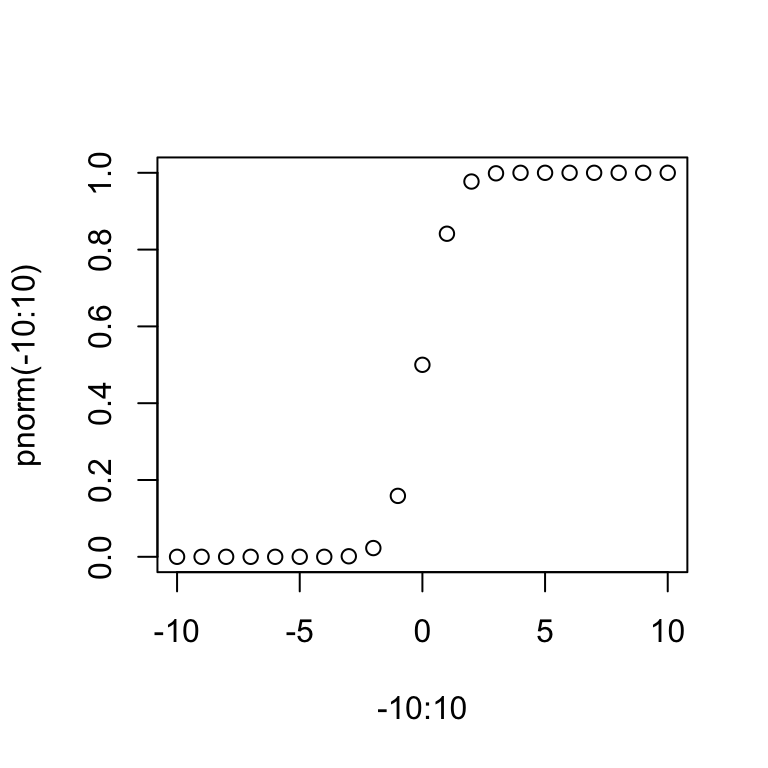
\includegraphics{InferenciaEstadistica_files/figure-latex/unnamed-chunk-153-1} \end{center}

O bien graficar la función de distribución de una normal entre -10 y 10:

\begin{Shaded}
\begin{Highlighting}[]
\KeywordTok{plot}\NormalTok{(}\OperatorTok{-}\DecValTok{10}\OperatorTok{:}\DecValTok{10}\NormalTok{,}\KeywordTok{dnorm}\NormalTok{(}\OperatorTok{-}\DecValTok{10}\OperatorTok{:}\DecValTok{10}\NormalTok{))}
\end{Highlighting}
\end{Shaded}

\begin{center}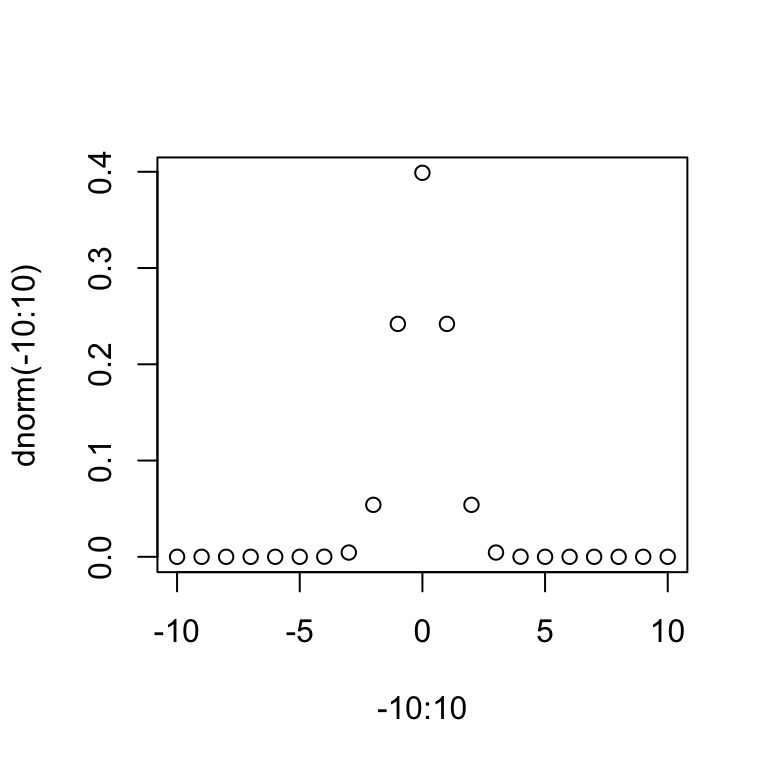
\includegraphics{InferenciaEstadistica_files/figure-latex/unnamed-chunk-154-1} \end{center}

¿Notas cómo nos faltan números en medio? Es porque el comando \texttt{-10:10} recorre los números entre -10 y 10 de 1 en 1.

\begin{Shaded}
\begin{Highlighting}[]
\DecValTok{-10}\OperatorTok{:}\DecValTok{10}
\end{Highlighting}
\end{Shaded}

{[}1{]} -10 -9 -8 -7 -6 -5 -4 -3 -2 -1 0 1 2 3 4 5 6 7 8
{[}20{]} 9 10

Para hacer más refinada la cantidad de puntos podemos hacer ahora una nueva secuencia pero yendo de 0.1 en 0.1:

\begin{Shaded}
\begin{Highlighting}[]
\NormalTok{x =}\StringTok{ }\KeywordTok{seq}\NormalTok{(}\OperatorTok{-}\DecValTok{10}\NormalTok{,}\DecValTok{10}\NormalTok{,}\FloatTok{0.1}\NormalTok{)}
\end{Highlighting}
\end{Shaded}

Puedes ver cómo se guardaron estos valores (este documento nada más muestra los primeros 9 porque es desperdiciar mucho espacio poner los 201 valores que hizo R)

\begin{Shaded}
\begin{Highlighting}[]
\NormalTok{x}
\end{Highlighting}
\end{Shaded}

{[}1{]} -10.0 -9.9 -9.8 -9.7 -9.6 -9.5 -9.4 -9.3 -9.2

¡La gráfica ahora se ve genial!

\begin{Shaded}
\begin{Highlighting}[]
\KeywordTok{plot}\NormalTok{(x,}\KeywordTok{dnorm}\NormalTok{(x))}
\end{Highlighting}
\end{Shaded}

\begin{center}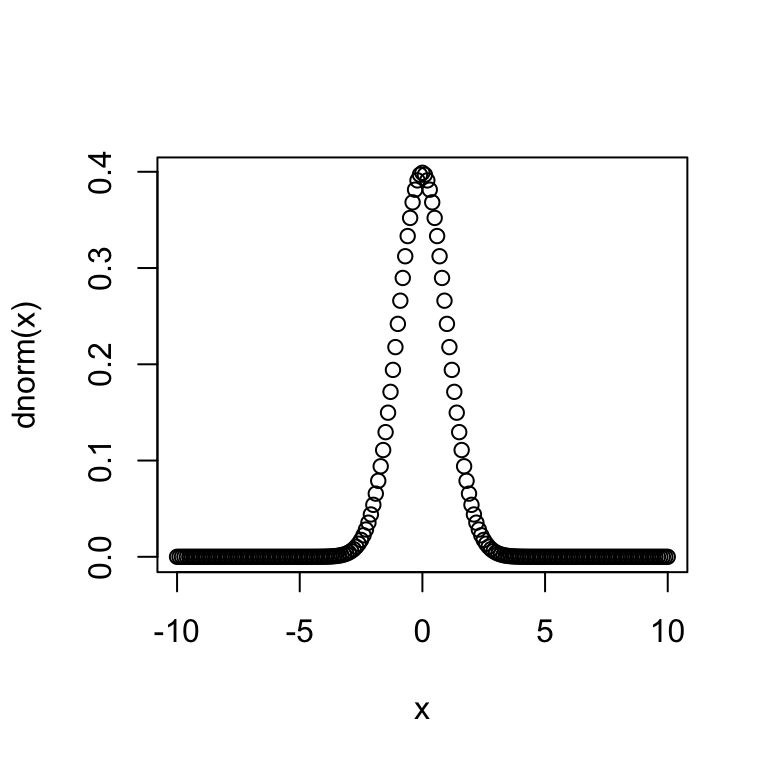
\includegraphics{InferenciaEstadistica_files/figure-latex/unnamed-chunk-159-1} \end{center}

\hypertarget{las-semillas}{%
\section{Las semillas}\label{las-semillas}}

En el apartado anterior dijimos que los números de R no eran aleatorios sino pseudoaleatorios y que estos se generaban por medio de una función. Cuando estamos haciendo investigación con simulaciones, para que nuestro estudio sea reproducible, aunque usemos números aleatorios, debemos usar siempre los mismos. La semilla se asegura de ello. Para poner una semilla usa el comando \texttt{set.seed} y pon dentro un entero.

\begin{Shaded}
\begin{Highlighting}[]
\KeywordTok{set.seed}\NormalTok{(}\DecValTok{1234}\NormalTok{)}
\end{Highlighting}
\end{Shaded}

Obtengamos un número aleatorio normal:

\begin{Shaded}
\begin{Highlighting}[]
\KeywordTok{rnorm}\NormalTok{(}\DecValTok{1}\NormalTok{)}
\end{Highlighting}
\end{Shaded}

{[}1{]} -1.20707

\begin{Shaded}
\begin{Highlighting}[]
\KeywordTok{rnorm}\NormalTok{(}\DecValTok{1}\NormalTok{)}
\end{Highlighting}
\end{Shaded}

{[}1{]} 0.277429

Volvamos a poner la semilla y saquemos un tercero:

\begin{Shaded}
\begin{Highlighting}[]
\KeywordTok{set.seed}\NormalTok{(}\DecValTok{1234}\NormalTok{)}
\KeywordTok{rnorm}\NormalTok{(}\DecValTok{1}\NormalTok{)}
\end{Highlighting}
\end{Shaded}

{[}1{]} -1.20707

¿Notas que es el mismo número que al inicio?

\hypertarget{ejercicio-5}{%
\section{Ejercicio 5}\label{ejercicio-5}}

Considera una población cuyo peso se distribuye normal con media 69 y desviación estándar 4.7. Esa misma población tiene una altura normal con media 1.8 \(m^2\) y desviación estándar de \(0.05\). Simula su índice de masa corporal. Calcula la media y desviación estándar del mismo. ¡No te olvides de usar una semilla!

\hypertarget{ejercicio-6}{%
\section{Ejercicio 6}\label{ejercicio-6}}

Un grupo de investigadores ha decidido que el índice de masa corporal tiene una distribución Cauchy y han simulado el índice de masa corporal como sigue:

\begin{Shaded}
\begin{Highlighting}[]
\KeywordTok{set.seed}\NormalTok{(}\DecValTok{6207}\NormalTok{)}
\CommentTok{#Simular IMC}
\NormalTok{imc <-}\StringTok{ }\KeywordTok{rcauchy}\NormalTok{(}\DecValTok{100}\NormalTok{,}\DecValTok{25}\NormalTok{,}\FloatTok{0.9}\NormalTok{)}

\CommentTok{#Calcular la media}
\KeywordTok{mean}\NormalTok{(imc)}
\end{Highlighting}
\end{Shaded}

El código es correcto. Pero la hipótesis de la distribución Cauchy no. Calcula la media varias veces usando diferentes semillas ¿Cuál es el problema? ¿Ocurre lo mismo si calculas la mediana?

  \bibliography{book.bib,packages.bib}

\end{document}
